\documentclass[13pt, a4paper, oneside]{Thesis} % Paper size, default font size and one-sided paper
\graphicspath{{./Pictures/}} % Specifies the directory where pictures are stored
\usepackage[square, numbers, comma, sort&compress]{natbib}
\hypersetup{urlcolor=blue, colorlinks=true} % Colors hyperlinks in blue - change to black if annoying
\title{\ttitle} % Defines t1he thesis title - don't touch this
\usepackage[utf8]{vietnam}
\usepackage{ucs}
\usepackage[grey,utopia]{quotchap}
\usepackage{amsmath}
\usepackage{graphicx}
\usepackage{wrapfig}
\usepackage{tikz}
%\pdfcryptsetup{owner=duythien,user=duythien}
\usepackage{relsize} %lam ky tu toan hoc small,big xem 5.24
\begin{document}

\frontmatter % Use roman page numbering style (i, ii, iii, iv...) for the pre-content pages
\begin{titlepage}

\newcommand{\HRule}{\rule{\linewidth}{0.5mm}} % Defines a new command for the horizontal lines, change thickness here

\center % Center everything on the page 
%----------------------------------------------------------------------------------------
%	HEADING SECTIONS
%----------------------------------------------------------------------------------------
\textsc{\LARGE ĐẠI HỌC QUỐC GIA TP.HỒ CHÍ MINH }\\ % Name of your university/college
\textsc{\LARGE TRƯỜNG ĐẠI HỌC KHOA HỌC TỰ NHIÊN }\\[1.5cm] % Name of your university/college
\textsc{\Large Khoa Vật Lý-Vật Lý Kỹ Thuật}\\[0.5cm] % Major heading such as course name
\textsc{\large Chuyên Ngành vật Lý Lý Thuyết}\\[0.5cm] % Minor heading such as course title

%----------------------------------------------------------------------------------------
%	TITLE SECTION
%----------------------------------------------------------------------------------------

\HRule \\[0.4cm]
{ \huge \bfseries Tính Toán Cấu Trúc Vùng Năng Lượng Bằng Phương Pháp Kp và Ứng Dụng}\\[0.4cm] % Title of your document

\HRule \\[1.5cm]
 
%----------------------------------------------------------------------------------------
%	AUTHOR SECTION
%----------------------------------------------------------------------------------------

\begin{minipage}{0.4\textwidth}
\begin{flushleft} \large
\emph{Sinh Viên:}\\
Trần Duy Thiện% Your name
\end{flushleft}
\end{minipage}
~
\begin{minipage}{0.4\textwidth}
\begin{flushright} \large
\emph{Thầy Hướng Dẫn:} \\
Ph.D Huỳnh Thanh Đức % Supervisor's Name
\end{flushright}
\end{minipage}\\[8cm]
%----------------------------------------------------------------------------------------
%	DATE SECTION
%----------------------------------------------------------------------------------------
{\large \today}\\[2cm] % Date, change the \today to a set date if you want to be precise
%----------------------------------------------------------------------------------------
%	LOGO SECTION
%----------------------------------------------------------------------------------------
%\includegraphics{Logo}\\[1cm] % Include a department/university logo - this will require the graphicx package
%----------------------------------------------------------------------------------------
\vfill % Fill the rest of the page with whitespace
\end{titlepage}
\clearpage % Start a new page
%----------------------------------------------------------------------------------------
%	ACKNOWLEDGEMENTS
%----------------------------------------------------------------------------------------

\begin{center}
\fontsize{22pt}{19.5pt} \selectfont
\textbf{LỜI CẢM ƠN}
\end{center}
\fontsize{13pt}{19.5pt} \selectfont

Tôi xin bày tỏ lòng biết ơn chân thành và sâu sắc đến Thầy Huỳnh Thanh Đức, người đã tận tình hướng dẫn và tạo điều kiện thuận lợi cho tôi hoàn thành luận văn này.

Tôi xin chân thành cảm ơn Thầy Đoàn Trí Dũng đã chỉ dẫn cho tôi thêm nhiều kiến thức trong suốt thời gian tôi thực hiện luận văn tại phòng Vật lý lý thuyết và toàn thể thầy cô, Viện Vật lý Tp. Hồ Chí Minh$\dots$

Tôi xin cảm ơn các Thầy Vũ Quang Tuyên và các thầy cô thuộc Bộ môn Vật lý-Vật lý lý thuyết của Trường Khoa học Tự nhiên đã cho tôi những kiến thức nền tản để làm luận văn này

Cảm ơn những người bạn của tôi, đã quan tâm và giúp để tôi, cảm ơn Tiến và anh Quan khóa 07 đã giúp để tôi

Cuối cùng, tôi xin gởi lời cảm ơn đến Cha, Mẹ và gia đình, những người luôn động viên, ủng hộ tôi trong suốt quá trình học tập.

\begin{center}
\hspace{8.cm} \vspace{1. cm}HCM, 2013\\
\hspace{8.cm}\textbf{Trần Duy Thiện}
\end{center}
\thispagestyle{empty}
\clearpage % Start a new page


%----------------------------------------------------------------------------------------
%	LIST OF CONTENTS/FIGURES/TABLES PAGES
%----------------------------------------------------------------------------------------

\pagestyle{fancy} % The page style headers have been "empty" all this time, now use the "fancy" headers as defined before to bring them back

%\lhead{\emph{Contents}} % Set the left side page header to "Contents"
\tableofcontents % Write out the Table of Contents

%\lhead{\emph{List of Figures}} % Set the left side page header to "List of Figures"
\listoffigures % Write out the List of Figures

%\lhead{\emph{List of Tables}} % Set the left side page header to "List of Tables"
\listoftables % Write out the List of Tables

%----------------------------------------------------------------------------------------
%	ABBREVIATIONS
%----------------------------------------------------------------------------------------

\clearpage % Start a new page

\setstretch{1.5} % Set the line spacing to 1.5, this makes the following tables easier to read

%\lhead{\emph{Abbreviations}} % Set the left side page header to "Abbreviations"
\listofsymbols{ll} % Include a list of Abbreviations (a table of two columns)
{
\textbf{RPA} & \textbf{R}andom phase approximation \\
%\textbf{Acronym} & \textbf{W}hat (it) \textbf{S}tands \textbf{F}or \\HH &lỗ trống nặng\\
\textbf{LH} &\textbf{L}ỗ trống nhẹ\\
\textbf{SO} & \textbf{T}ương tác spin quỹ đạo\\
\textbf{MQW} & \textbf{N}hiều lớp màng mỏng nano phủ lên nhau\\
\textbf{IQE} & \textbf{H}iệu xuất lượng tử nội bộ \\
\textbf{CB} &\textbf{V}ùng dẫn\\
\textbf{VB} &\textbf{V}ùng hóa trị\\
}

%----------------------------------------------------------------------------------------
%	PHYSICAL CONSTANTS/OTHER DEFINITIONS
%----------------------------------------------------------------------------------------
%\begin{tiny}
%\end{tiny}
\clearpage % Start a new page

%\lhead{\emph{Physical}} % Set the left side page header to "Physical Constants"

\listofconstants{lrcl} % Include a list of Physical Constants (a four column table)
{
Vận tốc ánh sáng trong chân không & $c$ & $=$ & $2.997\ 924\ 58\times10^{8}\ \mbox{ms}^{-\mbox{s}}$\\
Hằng số Planck & $\hbar$ & $=$ & $6.626\ 068\ 057\times10^{-34}\ \mbox{J.s}$\\
Bán kính Borh &$a_0$ &$=$ &$0.529A^{0}=0.529\times 10^{-10}$\\
Điện tich điện tử &$-e$ &$=$&$-1.6\times10^{-19}C$\\
% Constant Name & Symbol & = & Constant Value (with units) \\
}

%----------------------------------------------------------------------------------------
%	SYMBOLS
%----------------------------------------------------------------------------------------

\clearpage % Start a new page

%s\lhead{\emph{Symbols}} % Set the left side page header to "Symbols"

\listofnomenclature{lll} % Include a list of Symbols (a three column table)
{
$m_0$ & khối lượng của điện tử tự do\\
$m*$ &khối lượng hiệu dụng của đien tu \\
$n$ &chỉ số đặc trưng của dãy năng lượng bao gồm cả chỉ số spin\\
$\Gamma$ &biểu diễn bất khả quy\\
$\sigma$ & chỉ số spin, và ma trận P\\
$\Psi$ &hàm sóng trong không gian 3 chiều\\
$[A,B]=AB-BA$ &giao hoán tử\\
$r=(x,y,z)$ &vị trí của vecto\\
$E$ &năng lượng\\
${A,B}=\frac{1}{2}(AB+BA)$ &tích trực tiếp của đối xứng\\
$\mathfrak{D}$ &toán tử phép quay Euler\\
$\mathbf{P},p$ &Xung lượng\\
$\mathbf{A}$ &Thế véctơ\\
$\delta(x)$ &Hàm delta Dirac\\
$\delta_{mn}$ &Ký hiệu Kronecker\\
$\mathbf{A}\times\mathbf{B}$ hoặc $[\mathbf{A}\mathbf{B}]$ &Tích véctơ\\
% Symbol & Name & Unit \\

& & \\ % Gap to separate the Roman symbols from the Greek

$\omega$ & angular frequency & rads$^{-1}$ \\
% Symbol & Name & Unit \\
}

%----------------------------------------------------------------------------------------
%	DEDICATION
%----------------------------------------------------------------------------------------

\setstretch{1.3} % Return the line spacing back to 1.3

\pagestyle{empty} % Page style needs to be empty for this page

%\dedicatory{For/Dedicated to/To my\ldots} % Dedication text

\addtocontents{toc}{\vspace{2em}} % Add a gap in the Contents, for aesthetics

%----------------------------------------------------------------------------------------
%	THESIS CONTENT - CHAPTERS
%----------------------------------------------------------------------------------------

\mainmatter % Begin numeric (1,2,3...) page numbering

\pagestyle{fancy} % Return the page headers back to the "fancy" style

% Include the chapters of the thesis as separate files from the Chapters folder
% Uncomment the lines as you write the chapters
%
%\begin{savequote}[8cm]
%  ``All changes, even the most longed for, have their melancholy;
%  for what we leave behind us is a part of ourselves; we must
%  die to one life before we can enter another.''
%  \qauthor{Anatole France}
%  `The moment a man starts to behave ridiculous to a woman
%  you know he is serious at it.Ž
%  \qauthor{Colette}
%\end{savequote}
\makeatletter
\chapter{Lời Mở đầu}
\label{Chapter0} % For referencing the chapter elsewhere, use \ref{Chapter1} 
\rhead{\bfseries Khóa Luận Tốt Nghiệp,Năm 2013}Ngày nay, hầu hết các công nghệ sử dụng trong các lĩnh vực công nghệ thông tin và điện tử là kết quả của quá trình ứng dụng tương tác của trường điện từ với vật chất, một dạng tương tác giữa vật chất và ánh sáng. Chúng ta có thể thấy chúng hiện diện khắp nơi quanh cuộc sống của chúng ta chẳng hạn như các đèn LED dùng trong hiển  thị thông tin trong quảng cáo hay thiết bị gia dụng điện, hay xa hơn là các cổng giao tiếp quang học trong mạng lưới cáp quang truyền dẫn internet tốc độ cao, cáp dẫn điện và lĩnh vực đo đạc cần độ chính xác cao$\dots$Ngoài ra trong thời gian tới sẽ ứng dụng rất mạnh vào công nghệ  lưu trữ và xử lý thông tin đặc biệt là công nghệ spin điện tử (spintronics). Do đó để hiểu được các tính chất quan học của chất bán dẫn đều quan trong đầu tiên là ta phải tính được cấu trúc vùng năng lượng.\\
Trong luận văn này, tôi sẽ trình bày phương pháp tính cấu trúc vùng năng lượng của chất bán dẫn bằng phương pháp kp. Sau khi có được cấu trúc vùng năng lượng rồi ta sẽ ứng dụng nó vào phương trình Bloch bán dẫn để tìm dòng điện tích, dòng spin cũng như độ phân cực của điện tử và lỗ trống.

\chapter{Các khái Niệm Cơ Bản}
  \label{Chapter1} % For referencing the chapter elsewhere, use \ref{Chapter1} 
  \rhead{\bfseries Khóa Luận Tốt Nghiệp,Năm 2013}

  Để hiểu được tính chất vật lý của chất rắn mà cụ thể ở đây là chất bán dẫn việc tính  cấu trúc vùng năng lượng $\mathbf{E_n(k)}$ là hết sức quan trọng, và nó thể hiện hầu hết các tính chất điện và quang của vật liệu. Do tính chất tuần hoàn của mạng tinh thể, không gian xung lượng của hệ cũng có tính chất tuần hoàn, do đó cấu trúc vùng năng lượng chỉ cần xác định một khoãng hữu hạng k, và nếu như xét trong chất bán dẫn thì ta chỉ quan tâm một vài vùng ở cuối cùng bị lấp đầy, gọi là vùng hóa trị và một vài dải năng lượng đầu tiên còn trống gọi là vùng dẫn. Khi một vị trí trên vùng dẫn có electron thì ta có một hạt dẫn điện mang điện tích âm, khi một vị trí trên vùng cấm nó không có electrong nó tương đương với một hạt điện tích dương ở đó và được gọi là lỗ trống (hole), nó có ích khi ta tính các dòng. 
  Trong vật lý nguyên tử số hạng tương tác spin-orbit (SO) trong Hamiltonian được dẫn ra gần đúng từ phương trình Dirac [6] và đại lượng đó có giá trị sau
  \begin{equation}
  \mathcal{H}_{SO} = \frac{\hbar}{4m^2_0}\boldsymbol{\sigma} \cdot \left(\boldsymbol{\nabla} V_0\times \boldsymbol{p} \right) =  \frac{\hbar}{4m^2_0}\left(\boldsymbol{\sigma}\times \boldsymbol{\nabla}V_0\right)\cdot\boldsymbol{p}
  \end{equation}
  ở đây $\hbar$ là hằng số Planck, $m_0$ là khối lượng hiệu dụng của điện tử tự do, c là vận tốc ánh sáng, $\mathbf{p}$ là toán tử động lượng, $\mathbf{V}_0$ là thế Coulomb của nguyên tử và $\boldsymbol{\sigma} = \left(\sigma_x,\sigma_y,\sigma_z\right)$ là một véctơ ma trận Pauli và ta cũng biết rằng tương tác này làm thây đổi phổ năng lượng, làm tách spin.
  \section{Tương tác spin-orbit trong tinh thể chất rắn}
  Trong tinh thể chất rắn, phương trình chuyển động của điện tử có thể được miêu tả bởi cấu trúc vùng năng lượng $\mathbf{E}_n\left(\mathbf{k}\right)$, trong đó n là chỉ số đặc trưng(chỉ số vùng) cho giá trị khác nhau của $\mathbf{E}_n(\mathbf{k})$, ứng với mỗi giá trị của $\mathbf{k}$ (véctơ sóng), và ở đây số hạng tương tác SO cũng ảnh hưởng rất lớn đến cấu trúc vùng năng lượng  $\mathbf{E}_n\left(\mathbf{k}\right)$, ví dụ trong chất bán dẫn GaAs số hạng tương tác SO sẽ làm suy biến các mức năng lượng của spin up và spin down của tán sắc năng lượng, sự tách này là khá nhỏ cở một vài $meV$. Người ta đã ứng dụng hiệu ứng này vào việc tạo ra dòng photocurrent, tức là sinh ra dòng điện hoặc dòng spin trong chất bán dẫn bằng kích thích quang học thuần túy,trong mô hình 8$\times$8 kp có cả spin-orbit về mặt nguyên tắc là không suy biến và không thể viết 2 ma trận khối 4$\times$4.\\
  Tuy nhiên khi tính toán ta bỏ qua  một số hạng thứ 2 trong phương trình (4.4) thì mô hình trở thành suy biến, số hạng này được tham số hóa bởi tham số C trong mô hình Kane mở rộng, nếu tính đầy đủ thông số này nó sẽ gây ra một sự tách suy biến cở 0,1 $meV$ theo phương [110] nó là khá nhỏ có thể bỏ qua được nếu ta so sánh nó với mô hình kp 14$\times$14 tính đến cả tương tác vùng dẫn $p^*$ cho sự tách suy biến vào cỡ 1 $meV$ gần khe vùng. Từ mô hình kp 14$\times$14 ta có thể nhận lại mô hình kp 8$\times$8 nếu bỏ qua tương tác với vùng dẫn $p^*$ cụ thể là cho các thông số $P^{'}$, Q, và $\Delta^{-}$ trong phương trình (4.5) bằng 0.\\
  Các chất bán dẫn là tinh thể của các nguyên tử nhóm IV (Si,Ge) hay hợp chất của nhóm nguyên tử III và V(GaAs ,InSb) đặc điểm chung của chúng là lớp vỏ ngoài cùng không lắp đầy có thể là 3,4,5. điện tử phân bố trên 2 phân lớp s,p ví dụ: Si là ............... $3s^23p^2$ (nó chuyển thành$\dots 3s^13p^3$ khi liên kết các nguyên tử Si khác trong tinh thể ), như vậy khi một nguyên tử trong chất bán dẫn làm gì thì làm khi liên kết với nhau thì lớp vỏ ngoài của điện tử của nó được lắp đầy với 8 điện tử cụ thể là có 2 điện tử ở trạng thái s và 6 điện tử ở trạng thái p. Nhưng các trạng thái s và p không còn là trạng thái s và p của đơn nguyên tử  nữa \emph{mà là trạng thái s và p dùng chung của từng cặp nguyên tử}, hàm sóng mới là của trạng thái mới là tổ hợp tuyến tính (chồng chập) của hàm sóng điện tử của 2 nguyên tử, kết quả là 
  \begin{equation}
  \psi_+=\psi_1 +\psi_2  \qquad \psi_\_=\psi_1 -\psi_2
  \end{equation}
  chú ý ở trên ta viết một cách gần đúng lẽ ra phải có hằng số trước các hàm sóng $\psi_1$ và $\psi_2$ để cho dễ miêu tả (xem ở phụ lục), trong  đó $\psi_1,\psi_2$ là trạng thái điện tử của nguyên tử 1 và 2, trạng thái $\psi_+$ gọi là trạng thái liên kết(bonding) còn trạng thái $\psi_\_$ gọi là trạng thái phản liên kết(antiboding), dấu trừ hay dấu cộng là do hàm hám sóng $\psi_1,\psi_2$ có thể dương hay âm tùy ý vì chỉ có bình phương môđun hàm sóng mới có ý nghĩa vật lý.\\
  Biết hàm sóng thì ta có thể tính được năng lượng của trạng thái liên kết và phản liên kết, kết quả là từ 2 mức năng lượng s và p ta có 4 mức năng lượng sếp từ thắp đến cao s-boding,p-bonding và s-antibonding,p-antibonding, 2 mức thắp nhất là s-bonding, p-bonding lắp đầy với 8 điện tử. Cần chú ý rằng khi chuyển sang giải thích tinh thể bán dẫn thì ta chỉ quan tâm tới p-bonding có 6 trạng thái đã bị lấp đầy bởi 6 điện tử (nó sẽ chuyển thành vùng hóa trị suy biến 6 đã bị lấp đầy) và s-antibonding có 2 trạng thái trống, không có điện tử nào (nó sẽ chuyển thành vùng dẫn suy biến 2 còn trống). \emph{Tóm lại bây giờ chỉ còn 6 điện tử và 8 trạng thái chứ không phải 8 điện tử}.\\
  \begin{figure}[hc]
  \centering
  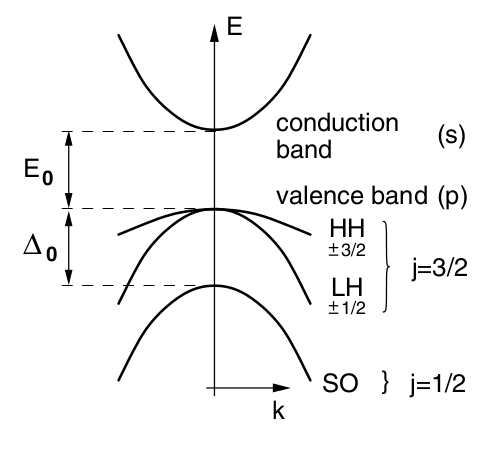
\includegraphics[width=0.50\textwidth]{./Figures/band1.png}
  %\rule{35em}{0.5pt}
  \caption[band structure]{Độ tách suy biến mức năng lượng do tương tác spin-orbit Ref [22]}
  \label{fig:band structure}
  \end{figure}
  Do tương tác của spin-orbit, các trạng thái ứng với $j=1/2$ bị tách suy biến có mức năng lượng thắp hơn năng lượng của trạng thái $j=3/2$, vùng năng lượng ứng với $j=1/2$ gọi là vùng hóa trị SO đôi khi người ta gọi nó là (split-off valence band)[15]. Vùng này suy biến bậc 2 theo hình chiếu của $j$ lênh trục $\mathbf{z}$ là $m_j=\pm 1/2$, vùng hóa trị ứng với $j=3/2$ gồm có 4 trạng thái ứng với các hình chiếu của $j$ lên trục $\mathbf{z}$ là $ m_j=\pm 3/2,\pm 1/2$, trong đó trạng thái ứng với $m_j=\pm 3/2$ là suy biến có cùng mức năng lượng và còn gọi là vùng lỗ trống nặng (heavy-hole) và $m_j = \pm 1/2$ là suy biến có cùng mức năng lượng và còn gọi là vùng lỗ trống nhẹ (light-hole), chú ý nếu như trong bán dẫn khối vùng lỗ trống nhẹ và lỗ trống nặng trùng nhau nên có suy biến bậc bốn.
  \section{Tương tác trao đổi}
  Tương tác trao đổi là kết quả của tương tác tĩnh điện Coulomb giữa những điện tử, do hàm sóng mô tả một cặp điện tử là hàm phản xứng nên nếu spin của hai điện tử là song song, phần tọa độ của hàm sóng phải là phản đối xứng:$\psi_{\uparrow\uparrow}\left(\mathbf{r}_1,\mathbf{r}_2\right)=-\psi_{\uparrow\uparrow}\left(\mathbf{r}_2,\mathbf{r}_1\right)$. Trường hợp ngược lại nếu spin của 2 điện tử là phản song song thì phần tọa độ của hàm sóng phải là đối xứng $\psi_{\uparrow\downarrow}\left(\mathbf{r}_1,\mathbf{r}_2\right)=-\psi_{\uparrow\downarrow}\left(\mathbf{r}_2,\mathbf{r}_1\right)$. vì vậy khả năng để 2 điện tử đến trong trường hợp sau là lớn hơn so vớ trường hợp trước, so với những điện tử có spin phản song thì spin điện tử song song cách xa hơn do đó lực đẩy giữa chúng là nhỏ hơn cũng như tương tác trao đổi tĩnh điện nhỏ hơn.\\
  Trong chất bán dẫn tương tác trao đổi thường không đóng góp lớn, ngoại trừ đối với những chất bán dẫn từ (CdMnTe) và mặt phân giới bán dẫn. 
  \section{Tương tác hyperfine với spin của hạt nhân}
  Đây là tương tác từ giữa spin của hạt nhân với spin của điện tử, tương tác này sẽ quan trọng nếu mang hạt hạt nhân trong chất bán dẫn có spin khác không như GaAs. Nếu hạt nhân này phân cực tương tác này tương đương với một từ trường hiệu dụng của hạt nhân tác dụng lên spin của điện tử. Trong GaAs khi $100\%$ hạt nhân phân cực từ trường này có giá trị hiệu dụng vài Tesla. Cũng như tương tác spin-orbit tương tác hyperfine tăng mạnh trong những nguyên tử có Z lớn, ngoài ra còn có tương tác từ đây là tương tác giữa mômen của một cặp điện tử, tương tác này rất yếu nó thường không được xét trong chất bán dẫn.
 


  \section{Lý thuyết nhóm trong vật lý}
  \subsection{Định nghĩa nhóm}
  Một tập hơp $\mathcal{G} =\{ a,b,c\ldots \}$ được gọi là một nhóm nếu nó tồn tại một phép nhân nhóm thỏa mản các tiên đề sau:
  \begin{enumerate}
  \item[1/] a,b $\in$ $\mathcal{G}$;\qquad\qquad c=a.b$\in \mathcal{G}$ \qquad\qquad\qquad\qquad(\emph{tính đóng})
  \item[2/] a,b,c $\in \mathcal{G}$;\qquad (ab).c=a.(b.c) \qquad\qquad\qquad\qquad (\emph{tính kết hợp})
  \item[3/]$\exists e \in\mathcal{G};\qquad g.e=e.g=g \qquad\forall g\in\mathcal{G}$ \  \qquad\qquad(\emph{phần tử đợn vị e duy nhất})
  \item[4/]$\forall a\in \mathcal{G} \qquad \exists b\in\mathcal{G}$;\qquad a.b=e ie, b=$a^{-1}$\qquad\qquad (\emph{phần tử nghịch đảo})
  \end{enumerate}
  \subsection{Nhóm điểm}
  $1/$ \textbf{Nhóm trực giao} $\mathcal{O}(3)$ \textbf{trong không gian 3 chiều}:
  \begin{equation}
  \mathcal{O}(3) = \{\mathcal{O}=\mathcal{O}_{ij}:\mathcal{O}_{ij}\in\mathcal{R},1\leq i,j\leq 3 ,\mathcal{O}^T\mathcal{O}=\mathbb{E}_3\}
  \end{equation}
  trong đó $\mathbb{E}_3$ là ma trận đơn vị, ta có thể chứng minh $det(\mathcal{O})=\pm1$,và nhóm $\mathcal{SO}(3)$ là nhóm con bất biến thậm chí là chuẩn tắc, các phần tử của nó là các phép quay trong không gian 3 chiều còn các phần tử của lớp kề nó là phép quay kèm theo một phép đối xứng gương [21]
  \begin{equation}
  \mathcal{SO}(3) = \{\mathcal{O}\in\mathcal{O}(3):det(\mathcal{O})=1\}
  \end{equation}
  Ý nghĩa hình học của nhóm $\mathcal{SO}(3)$: Ta có thể chứng minh nếu $\mathcal{O}\in\mathcal{SO}(3)$ thì tồn tại một véctơ $\vec{f}$ sao cho:
  \begin{equation}
  \mathcal{O}\vec{f}=1.\vec{f} \qquad |\vec{f}|=1
  \end{equation}
  ta chọn hệ trực chuẩn $\mathbf{f}_1,\mathbf{f}_2,\mathbf{f}_3$, hệ trực chuẩn ở đây có ý nghĩa là $\langle \mathbf{f}_i,\mathbf{f}_j\rangle=\delta_{ij}$, ta sẽ tìm dạng ma trận $\mathcal{O}$ trong cơ sở này, để tìm nó ta giải hệ phương trình sau:
  \begin{equation}
  \begin{cases} 
  \mathcal{O}\mathbf{f}_1 &=\alpha_1\mathbf{f}_1 +\beta_1\mathbf{f}_2 +\gamma_1\mathbf{f}_3 \\
   \mathcal{O}\mathbf{f}_2 &=\alpha_2\mathbf{f}_1 +\beta_2\mathbf{f}_2 +\gamma_2\mathbf{f}_3  \\
   \mathcal{O}\mathbf{f}_3 &=\alpha_3\mathbf{f}_1 +\beta_3\mathbf{f}_2 +\gamma_3\mathbf{f}_3 
   \end{cases} 
   \end{equation}
  giải hệ phương trình trên ta có kết qủa của ma trận $\mathcal{O}$ như sau:
  \begin{equation}
  \mathcal{O}=\mathcal{C}_3(\alpha)=\begin{pmatrix}
  \cos\alpha &-sin\alpha & 0\\
  \sin\alpha &\cos\alpha &0\\
  0 &0 &1
  \end{pmatrix}
  \end{equation}
  %-----------------------------Hinh coordinte-------------------------

  \begin{figure}[hc]
  \centering
  \ifx\du\undefined
    \newlength{\du}
  \fi
  \setlength{\du}{15\unitlength}
  \begin{tikzpicture}
  \pgftransformxscale{1.000000}
  \pgftransformyscale{-1.000000}
  \definecolor{dialinecolor}{rgb}{0.000000, 0.000000, 0.000000}
  \pgfsetstrokecolor{dialinecolor}
  \definecolor{dialinecolor}{rgb}{1.000000, 1.000000, 1.000000}
  \pgfsetfillcolor{dialinecolor}
  \pgfsetlinewidth{0.100000\du}
  \pgfsetdash{}{0pt}
  \pgfsetdash{}{0pt}
  \pgfsetbuttcap
  {
  \definecolor{dialinecolor}{rgb}{0.000000, 0.000000, 0.000000}
  \pgfsetfillcolor{dialinecolor}
  % was here!!!
  \pgfsetarrowsend{latex}
  \definecolor{dialinecolor}{rgb}{0.000000, 0.000000, 0.000000}
  \pgfsetstrokecolor{dialinecolor}
  \draw (22.900000\du,12.950000\du)--(30.900000\du,12.950000\du);
  }
  \pgfsetlinewidth{0.100000\du}
  \pgfsetdash{}{0pt}
  \pgfsetdash{}{0pt}
  \pgfsetbuttcap
  {
  \definecolor{dialinecolor}{rgb}{0.000000, 0.000000, 0.000000}
  \pgfsetfillcolor{dialinecolor}
  % was here!!!
  \pgfsetarrowsend{latex}
  \definecolor{dialinecolor}{rgb}{0.000000, 0.000000, 0.000000}
  \pgfsetstrokecolor{dialinecolor}
  \draw (22.900000\du,12.950000\du)--(22.950000\du,5.300000\du);
  }
  \pgfsetlinewidth{0.100000\du}
  \pgfsetdash{}{0pt}
  \pgfsetdash{}{0pt}
  \pgfsetbuttcap
  {
  \definecolor{dialinecolor}{rgb}{0.000000, 0.000000, 0.000000}
  \pgfsetfillcolor{dialinecolor}
  % was here!!!
  \pgfsetarrowsend{latex}
  \definecolor{dialinecolor}{rgb}{0.000000, 0.000000, 0.000000}
  \pgfsetstrokecolor{dialinecolor}
  \draw (22.850000\du,12.900000\du)--(16.450000\du,16.600000\du);
  }
  \pgfsetlinewidth{0.050000\du}
  \pgfsetdash{}{0pt}
  \pgfsetdash{}{0pt}
  \pgfsetmiterjoin
  \pgfsetbuttcap
  {
  \definecolor{dialinecolor}{rgb}{0.000000, 0.000000, 0.000000}
  \pgfsetfillcolor{dialinecolor}
  % was here!!!
  \pgfsetarrowsend{latex}
  \definecolor{dialinecolor}{rgb}{0.000000, 0.000000, 0.000000}
  \pgfsetstrokecolor{dialinecolor}
  \pgfpathmoveto{\pgfpoint{21.150000\du}{8.650000\du}}
  \pgfpathcurveto{\pgfpoint{23.350000\du}{9.650000\du}}{\pgfpoint{27.250000\du}{8.600000\du}}{\pgfpoint{23.700000\du}{7.250000\du}}
  \pgfusepath{stroke}
  }
  % setfont left to latex
  \definecolor{dialinecolor}{rgb}{0.000000, 0.000000, 0.000000}
  \pgfsetstrokecolor{dialinecolor}
  \node[anchor=west] at (22.800000\du,4.400000\du){$\mathbf{f_3}$};
  % setfont left to latex
  \definecolor{dialinecolor}{rgb}{0.000000, 0.000000, 0.000000}
  \pgfsetstrokecolor{dialinecolor}
  \node[anchor=west] at (16.900000\du,17.300000\du){$\mathbf{f_1}$};
  % setfont left to latex
  \definecolor{dialinecolor}{rgb}{0.000000, 0.000000, 0.000000}
  \pgfsetstrokecolor{dialinecolor}
  \node[anchor=west] at (30.200000\du,13.950000\du){$\mathbf{f_2}$};
  % setfont left to latex
  \definecolor{dialinecolor}{rgb}{0.000000, 0.000000, 0.000000}
  \pgfsetstrokecolor{dialinecolor}
  \node[anchor=west] at (22.850000\du,13.700000\du){O};
  \end{tikzpicture}
  \caption[phép quay trục $f_3$]{Phép quay quanh trục$\mathbf{f_3}$ }
  \label{fig:phép quay trục $f_3$}
  \end{figure}

  như vậy ma trận $\mathcal{O}$ chính là ma trận của phép quay quanh trục $\mathbf{f}_3$ một góc $\theta$, quay theo quy tắc bàn tay phải,làm tương tự cho các trục quay $\mathbf{f}_1,\mathbf{f}_2$ ta có kết quả sau:
  \begin{equation}
  \mathcal{O}=\mathcal{C}_2(\beta)=\begin{pmatrix}
  \cos\beta &0 &sin\beta\\
  0 &1 & 0\\
  -\sin\beta &0 &\cos\beta
  \end{pmatrix}
  \end{equation}
  \begin{equation}
  \mathcal{O}=\mathcal{C}_2(\gamma)=\begin{pmatrix}
  1 &0 &0 \\
  0 &\cos\gamma &-\sin\gamma\\
  0 &\sin\gamma &\cos\gamma
  \end{pmatrix}
  \end{equation}
  Thông thường các hệ số 1,2,3 được thây bởi $\mathit{x,y,z}$ trong khi ta thực hành trên các bài toán vật lý, xét nhóm quay trong không gian ba chiều $\mathcal{SO}(3)$. Mọi phép quay không gian ba chiều quanh gốc tọa độ $\mathbf{O}$ đều có thể được thực hiện dưới dạng tổ hợp của ba phép quay liên tiếp sau đây: phép quay góc $\alpha$ quanh trục $\mathbf{O}\mathit{z}$ chuyển các trục tọa độ $\mathbf{O}\mathit{x}$ và $\mathbf{O}\mathit{y}$ thành $\mathbf{O}\mathit{x}^{'}$ và $\mathbf{O}\mathit{y}^{'}$, 
  phép quay góc $\beta$ quanh trục mới $\mathbf{O}\mathit{y}^{'}$ chuyển
  các trục mới $\mathbf{O}\mathit{z}$ và $\mathbf{O}\mathit{x}$ thành $\mathbf{O}\mathit{z}^{'}$ và $\mathbb{O}\mathit{x}^{''}$, phép quay góc $\gamma$ quanh trục mới $\mathbf{O}\mathit{z}^{'}$ (xem hình 2.11). Ba thông
  số $\alpha,\beta,\gamma$ gọi là ba góc Euler và . Ký hiệu phép quay với ba góc Euler $\mathfrak{D}(\alpha,\beta,\gamma)$\\
  \begin{enumerate}
  \item[1.] Thực hiện phép quay 1 góc $\alpha$ quanh trục $\mathcal{O}z\qquad\sum\longrightarrow\sum^{'},0\leq \alpha\leq 2\pi$ 
  \item[2.] Thực hiện phép quay 1 góc $\beta$ quanh trục $\mathcal{O}y^{'}\qquad\sum^{'}\longrightarrow\sum^{''},0\leq \alpha\leq \pi$ 
  \item[3.] Thực hiện phép quay 1 góc $\gamma$ quanh trục $\mathcal{O}z^{'}\qquad\sum^{''}\longrightarrow\sum^{'''},0\leq \gamma\leq 2\pi$ 
  \end{enumerate}

  \begin{figure}[hc]
  \centering
  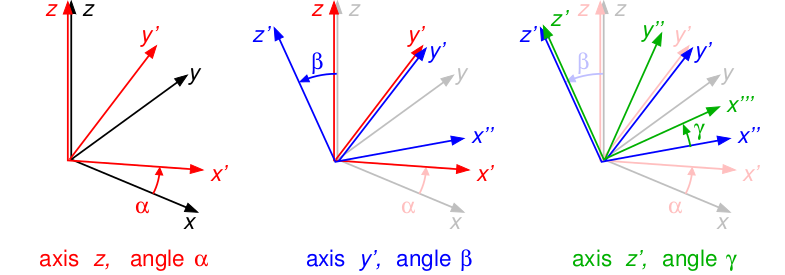
\includegraphics[width=0.70\textwidth]{./Figures/Selection_001.png}
  %\rule{35em}{0.5pt}
  \caption[phép quay]{Phép quay quanh trục$\mathcal{O}z,\mathcal{O}y^{'},\mathcal{O}z^{'}$ }
  \label{fig:phép quay}
  \end{figure}
  \begin{align}
  \mathfrak{D}(\alpha,\beta,\gamma)&=
  \mathfrak{D}_z(\alpha)\mathfrak{D}_y(\beta)\mathfrak{D}_z(\gamma)\notag\\
  &=\begin{pmatrix}
  \cos\alpha &-sin\alpha & 0\\
  \sin\alpha &\cos\alpha &0\\
  0 &0 &1
  \end{pmatrix}
  \begin{pmatrix}
  \cos\beta &0 &sin\beta\\
  0 &1 & 0\\
  -\sin\beta &0 &\cos\beta
  \end{pmatrix}
  \begin{pmatrix}
  \cos\alpha &-sin\alpha & 0\\
  \sin\alpha &\cos\alpha &0\\
  0 &0 &1
  \end{pmatrix}\\
  &=\begin{pmatrix}
  \cos\alpha\cos\beta\cos\gamma -\sin\alpha\sin\gamma & \cos\alpha\cos\beta\sin\gamma +\sin\alpha\sin\gamma & -\cos\alpha\sin\beta \\
  -\sin\alpha\cos\beta\cos\gamma -\cos\alpha\sin\gamma & -\sin\alpha\cos\beta\sin\gamma +\cos\alpha\sin\gamma &\sin\alpha\sin\beta \\
  \sin\beta\cos\gamma &\sin\beta\sin\gamma & \cos\beta \notag
  \end{pmatrix}
  \end{align}
  \section{Phép quay trong cơ học lượng tử}
  \textbf{1.Toán tử của phép quay:} Với bất kỳ phép quay trong hệ vật lý chúng ta có thể biểu diễn mối liên hệ giữa toán tử phép quay $\mathfrak{D}(R)$ và trạng thái của hệ vật lý sau khi thực hiện phép quay như sau:
  \begin{equation}
  \vert \Psi\rangle_{R} = \mathfrak{D}(R) \vert \Psi\rangle_{R}
  \end{equation}  
  ta sẽ dẫn ra dạng toán tử phép quay $\mathfrak{D}(R)$,gọi $\mathfrak{D}(\mathbf{n},d\phi)$ là toán tử của phép quay quanh hệ một góc $d\phi$ vô cùng bé quanh một trục có véctơ đơn vị là $\mathbf{n}$, trong phép quay này tọa độ của hạt trong hệ biến đổi như sau:
  \begin{equation}
  \mathbf{r_i} \longrightarrow \mathbf{r}_i^{'} = \mathbf{r_i} +d\mathbf{r_i} \qquad i=1,2,\dots, N
  \end{equation} 
  trong đó $d\phi = d\phi\left(n\times r_i\right)$, khai triển hàm sóng $\vert \Psi\rangle$ quanh điểm $d\mathbf{r}_i$  và chỉ lại số hạng bậc nhất sau vài phép biến đổi ta có dạng toán tử $\mathfrak{D}(\mathbf{n},d\phi)$ như sau:
  \begin{equation}
  \mathfrak{D}(\mathbf{n},d\phi) = 1 -i\left(\frac{\mathcal{J}\mathbf{n}}{\hbar}\right)d\phi
  \end{equation}
  ở đây ta sẽ định nghĩa đại lượng $\mathcal{J}$ là toán tử mômen động lượng toàn phần và $\mathcal{J}$ cũng gọi là một vi tử của phép quay quanh hệ một góc vô cùng bé \\
  Bây giờ ta xét hệ quay quanh 1 góc hữu hạn $\phi$ quanh trục $\mathbf{n}$ gọi $\mathfrak{D}(\mathbf{n},d\phi)$  là toán tử của phép quay này ta có:
  \begin{equation}
  \mathfrak{D}(\mathbf{n},\phi + d\phi) =\mathfrak{D}(\mathbf{n},d\phi)\mathfrak{D}(\mathbf{n},\phi)
  \end{equation}
  hoặc ta có thể biểu diễn dưới dạng sau:
  \begin{equation}
  \mathfrak{D}(\mathbf{n},d\phi) = \lim_{N\longrightarrow\infty}\left(1 -i\frac{\mathcal{J}\mathbf{n}}{\hbar}\frac{\phi}{N}\right)^N = exp\left(-i\phi\frac{\mathbf{n}\mathcal{J}}{\hbar}\right)
  \end{equation}
  \begin{figure}[hc]
  \centering
  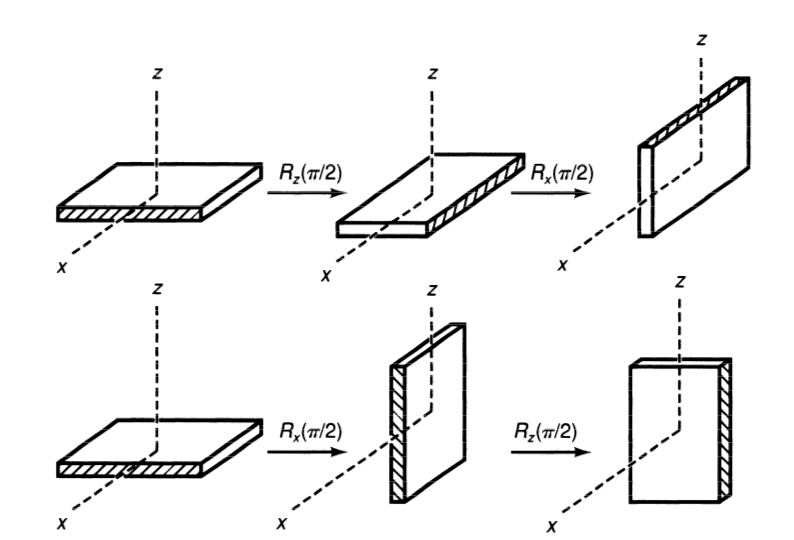
\includegraphics[width=0.70\textwidth]{./Figures/rota.png}
  %\rule{35em}{0.5pt}
  \caption[sự không giao hoán của phép quay]{Thí dụ minh họa sự không giao hoán của phép\\ quay quanh các trục của phép quay Ref [9] }
  \label{fig:sự không giao hoán của phép quay}
  \end{figure}\\
 Công thức (2.15) cho ta thấy các toán tử $\mathcal{J}_x,\mathcal{J}_y,\mathcal{J}_z$ là không giao hoán với nhau.\\
  \textbf{2.Phép quay là một nhóm:} Do đó nó đầy đủ tính chất nhóm tức tính đóng, tính kết hợp, tồn tại phần tử đơn vị và phần tử nghịch đảo. Một tập hợp các phép quay của toán tử của $\mathfrak{D}(R)$ cũng là một nhóm, xét 2 phép quay $\mathfrak{D}_1$,$\mathfrak{D}_2$ ta có thể tính nó như thế nào, dựa vào biểu thức (2.15) ta dễ dàng suy ra được tích $\mathfrak{D}_1 .\mathfrak{D}_2$ như sau:
  \begin{equation}
  \mathfrak{D}(R_2)\mathfrak{D}(R_1)=\mathfrak{D}(R_2 R_1)
  \end{equation} 
  sử dụng (2.14) khai triển nó tới số hạng $d\phi^2$ đồng thời sử dụng công thức sau [9]
  \begin{equation}
  \mathfrak{D}_x(\varepsilon)\mathfrak{D}_y(\varepsilon) -\mathfrak{D}_y(\varepsilon)\mathfrak{D}_x(\varepsilon) =\mathfrak{D}_z(\varepsilon^2)- \mathfrak{D}_{any}(0)
  \end{equation}
  ta dễ dàng có được điều này:
  \begin{equation}
  \left[ \mathcal{J}_i,\mathcal{J}_j\right] = i\hbar\varepsilon_{ijk}\mathcal{J}_k
  \end{equation}
  trong đó $\varepsilon_{ijk}$ là tenxo phản đối xứng được định nghĩa như sau. Gọi p là số hoán đưa (i,j,k) về tập hợp (1,2,3) khi đó:
  \begin{equation}
  \varepsilon_{ijk}=\begin{cases}
  &+1 \qquad \text{nếu} i\neq j\neq k \qquad \text{và p là số chẳn}\\
  &-1 \qquad \text{nếu} i\neq j\neq k \qquad \text{ và nếu p là số lẻ}\\
  & 0 \qquad \text{nếu có từ 2 chỉ số trở lên trùng nhau }
  \end{cases}
  \end{equation}
  \textbf{3.Hàm riêng và trị riêng của mômen động lượng toàn phần:} Dựa vào định nghĩa (2.19)  ta có thể tìm được trị riêng của $\mathcal{J}^2$ và $\mathcal{J}_z$  mà không cần phải biết dạng tường minh của 2 toán tử này, với mục đích đó ta đưa vào các toán tử thang $\mathcal{J}_{\pm}$ như sau:
  \begin{equation}
  \mathcal{J}_{\pm} =\mathcal{J}_x \pm \mathcal{J}_y 
  \end{equation}
  tác dụng toán tử $\mathcal{J}_{\pm}$ lên trạn thái $\vert j,m\rangle$ sau vài phép biến đổi ta có
  \begin{equation}
  \mathcal{J}_{\pm}\vert j,m\rangle = \sqrt{(j\mp m)(j\pm m+1)}\hbar\vert j,m\pm 1\rangle
  \end{equation}
  để cho biểu thức ket bên vế phải chuẩn hóa. ta cần phải giới hạn giá trị của m là (2$j$ +1)
  \begin{equation}
   m= -j,-j+1,\dots ,j-1,j
  \end{equation} 
  như vậy chỉ với lập luận dựa trên hệ thức giao hoán  và tính tự liên hợp của mômen động lượng ta đi đến những kết luận quan trọng sau đây:
  \begin{enumerate}
  \item[1.] Bình phương mômen động lượng bị lượng tử hóa theo quy tắc  $\mathcal{J}^2 = j(j+1)\hbar^2$, trong đó số lượng tử $j$ chỉ nhận những giá trị $j=0,1/2,1,3/2,2,5/2,\dots$
  \item[2.] Với $j$ cho trước tồn tại (2$j$+1) trạng thái $\vert j,m\rangle$ chú ý nó cũng là số chiều trong biễu diễn bất khả quy, và số lượng m được cho bởi công thức (2.32), hình chiếu mômen động lượng trên trục $z$ bị lượng tử hóa theo quy tắc $\mathcal{J}_z=m\hbar$. Ngoài ra còn có dạng ma trận của toán tử mômen động lượng, phép cộng mômen động lượng và hàm sóng của hạt có chứa spin $\dots$ thêm khảo thêm [3,9].
  \end{enumerate}
  \section{Lý thuyết nhiễu loạn giả suy biến}
  \textbf{Lý thuyết nhiễu loạn giả suy biến:} Đó là một phương pháp rất tổng quát và hữu ích để chúng ta tính toán gần đúng các thành phần không chéo hóa của Hamiltonian độc lập với thời gian, nhưng nó cũng có thể dùng cho nhiều trường hợp khác trong cơ học lượng tử, phương pháp này đôi khi người ta gọi là phương pháp L$\ddot{o}$wdin partitioning nội dung của phương pháp này như sau [10,11,22,23,24]:
  Thành phần Hamiltonian ta có thể tách ra hai thành phần, một thành phần $\mathcal{H}_0$ như ta đã biết là thành phần không nhiễu loạn có trị riêng năng lượng là $E_n$ và hàm riêng là $\vert \psi_n\rangle$, $\mathcal{H}^{'}$ là thành phần nhiễu loạn có thể xem số hạng $\mathbf{kp}$ trong phương trình (4.1) do đó ta có thể viết Hamiltonian như sau:
  \begin{equation}
  \mathcal{H} =\mathcal{H}_0 +\mathcal{H}^{'}
  \end{equation}
  Giả sử chúng ta có thể chia hàm riêng $\vert\psi_n\rangle$ ra làm 2 thành phần, một tập hợp thành phần lớp $\mathcal{A}$ và một tập hợp thành phần lớp $\mathcal{B}$, sao cho ta chỉ xét các thành phần tập hợp lớp $\mathcal{A}$ còn $\mathcal{B}$ ta có thể  bỏ qua chú ý ta chỉ bỏ qua $\mathcal{B}$ thôi còn các hiệu ứng giửa tập hợp $\mathcal{A}$ và $\mathcal{B}$ thì ta không bỏ qua, tức là các thành phần thuộc lớp $\mathcal{A}$ ta chọn như sau, bao gồm 2 lỗ trống nặng, 2 lỗ trống nhẹ và 2 spin-off band, còn tập hợp $\mathcal{B}$ là các thành phần còn lại.
  Lý thuyết nhiễu loạn giả suy biến xây dựng cơ bản dựa trên ý tưởng là toán tử Unitary $e^{-S}$ như vậy ta có thể thu được một Hamiltonians mới nhờ phép biến đổi sau:
  \begin{equation}
  \tilde{\mathcal{H}} =e^{-S}\mathcal{H}e^{S}
  \end{equation}
  trong thành phần ma trận $\langle\psi_m\vert \tilde{\mathcal{H}} \vert \psi_l\rangle$ khi ta xét đến số hạng nhiễu loạn $\mathcal{H}^{'}$ thì thành phần $\langle\psi_m\vert \mathcal{H}^{'} \vert \psi_l\rangle$ của tập hợp $\mathcal{B}$ sẽ triệt tiêu nếu ta xét trong các dãy  2 lỗ trống nặng, 2 lỗ trống nhẹ và 2 spin-off band, chúng ta có thể miêu tả loại bỏ các thành phần không chéo hóa trong $\mathcal{H}$ như hình vẽ dưới đây:
  \begin{figure}[hc]
  \centering
  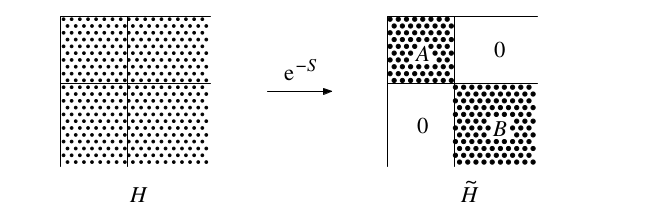
\includegraphics[width=0.70\textwidth]{./Figures/lowd.png}
  %\rule{35em}{0.5pt}
  \caption[Removal of off-diagonal elements of H]{Hamiltonian được đưa về dạng chéo hóa khối nhờ toán tử S,\\ gồm 2 thành phần $\mathcal{A},\mathcal{B}$ Ref[22]}
  \label{fig:Removal of off-diagonal elements of H}
  \end{figure}
  \begin{figure}[hc]
  \centering
  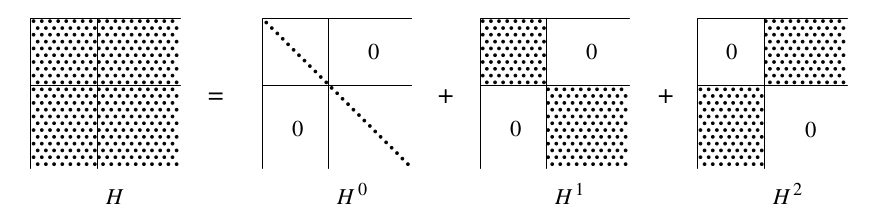
\includegraphics[width=0.70\textwidth]{./Figures/lowd2.png}
  %\rule{35em}{0.5pt}
  \caption[ Representation of H ]{Trình bày $\mathcal{H}$ thông qua các Hamiltionian $\mathcal{H}^0 + \mathcal{H}^1 +\mathcal{H}^2$ Ref[22]}
  \label{fig: Representation of H }
  \end{figure}
  Đại lượng S trong biểu thức (2.24) có nhiệm vụ biến đổi $\mathcal{H}^2$ về dạng tương tự như $\mathcal{H}^1$ trong khi vẫn giữ được hình thức chéo hóa khối của thành phần $\mathcal{H}^0+\mathcal{H}^1$ , để xác định đước toán tử S ta cần khai triển S dưới dạng chuổi Taylor như sau:
  \begin{equation}
  e^S = 1 +S + \frac{1}{2!}S^2 +\frac{1}{3!}S^3 +\dotsi
  \end{equation}
  và thây biểu thức này vào (2.24) ta có, chú ý rằng toán tử S là phản Hermitian tức $S^{\dagger} =-S$, ví dụ phép biến đổi từ biễu diễn Schr$\ddot{o}$dinger sang biễu diễn Heisenberg thì đại lượng S có giá trị là $\frac{i}{\hbar}Ht$
  \begin{equation}
  \tilde{\mathcal{H}} = \sum_{j=0}^{\infty}\frac{1}{j!}[\mathcal{H},S]^{j} = \sum_{j=0}^{\infty}\frac{1}{j!}[\mathcal{H}^0 +\mathcal{H}^1,S]^{j}+\sum_{j=0}^{\infty}\frac{1}{j!}[\mathcal{H}^2,S]^{j}
  \end{equation}
  ở đây giao hoán tử $\mathcal{A},\mathcal{B}$ được định nghĩa như sau:
  \begin{equation}
  [\mathcal{A},\mathcal{B}]^{j} = [\cdots\underbrace{[\mathcal{A},\mathcal{B}],\mathcal{B},\cdots \mathcal{B}}_{j\longrightarrow \infty}
  \end{equation}
  vì S làm cho thành phần không chéo hóa khối của $\mathcal{H}^2$ nên thành phần khối chéo hóa $\mathcal{H}_d$ có trong $\tilde{\mathcal{H}}$ gồm có $[\mathcal{H}^0 +\mathcal{H}^1,S]^{j}$ với j là chẵn còn sồ hạng $[\mathcal{H}^2,S]^{j}$ ới j là lẻ:
  \begin{equation}
  \tilde{\mathcal{H}}_d  = \sum_{j=0}^{\infty}\frac{1}{(2j)!}[\mathcal{H}^0 +\mathcal{H}^1,S]^{(2j)}+\sum_{j=0}^{\infty}\frac{1}{(2j+1)!}[\mathcal{H}^2,S]^{(2j+1)}
  \end{equation}
  ngược lại thành phần khối không chéo hóa $\mathcal{H}_n$ có trong $\mathcal{H}$ gồ có $[\mathcal{H}^0 +\mathcal{H}^1,S]^{j}$ với j là lẻ còn số hạng $[\mathcal{H}^2,S]^{j}$ với j là chẳn:
   \begin{equation}
  \tilde{\mathcal{H}}_n  = \sum_{j=0}^{\infty}\frac{1}{(2j+1)!}[\mathcal{H}^0 +\mathcal{H}^1,S]^{(2j+1)}+\sum_{j=0}^{\infty}\frac{1}{(2j)!}[\mathcal{H}^2,S]^{(2j)}
  \end{equation}
  vì theo đầu bài ta đã nói toán tử S được định nghĩa làm cho các thành phần khối không chéo hóa $\mathcal{H}_n =0$ là bằng không, ta chọn S tới số hạng bậc 3
  \begin{equation}
  S =S^{(1)} +S^{(2)} +S^{(3)} +\cdots
  \end{equation}  
  sử dụng biểu thức (2.31) kết hợp với $\mathcal{H}_n =0$ ta có kết quả sau:
  \begin{align}
  [\mathcal{H}^0,S^{(1)}] &= -\mathcal{H}^2 \notag\\
  [\mathcal{H}^0,S^{(2)}] &= -[\mathcal{H}^1,S^{(1)}] \notag\\
  [\mathcal{H}^0,S^{(3)}] &= -[\mathcal{H}^1,S^{(2)}] -\frac{1}{3}[[\mathcal{H}^2,S^{(1)}],S^{(2)}] \notag\\
  \cdots &= \cdots
  \end{align}
  giải phương trình (2.32) cho ta giá trị S cần tìm,gợi ý nhân 2 vế với két-véctơ và bra-véctơ $\vert nk\rangle$ và vì $\mathcal{H}^2$ ta có:
   \begin{align}
   S_{ml}^{(1)} &=-\frac{\mathcal{H}_{ml}^{'}}{E_m -E_l} \notag\\
   S_{ml}^{(2)}&= \frac{1}{E_m -E_l}\left[\sum_{m^{'}}\frac{\mathcal{H}_{mm^{'}}-\mathcal{H}_{m^{'}l}}{E_m^{'} -E_l}- \sum_{l^{'}}\frac{\mathcal{H}_{ml^{'}}-\mathcal{H}_{l^{'}l}}{E_m -E_{l^{'}}} \right]\notag\\
   S_{ml}^{(1)} &=\frac{1}{E_m -E_l}\notag\\
   &\times \biggl[-\sum_{m^{'},m^{''}}\frac{\mathcal{H}_{mm^{''}}\mathcal{H}_{m^{''}m}\mathcal{H}_{m^{'}l}}{(E_{m^{''}}-E_{l})(E_{m^{'}}-E_l)} 
  -\sum_{l^{'},l^{''}}\frac{\mathcal{H}_{ml^{'}}\mathcal{H}_{l^{'}l^{''}}\mathcal{H}_{l^{''}l}}{(E_{m^{'}}-E_{l^{''}})(E_{m}-E_l^{'})} \notag\\
  &+\sum_{l^{'},m^{'}}\frac{\mathcal{H}_{mm^{'}}\mathcal{H}_{m^{'}l^{'}}\mathcal{H}_{l^{'}l}}{(E_{m^{'}}-E_{l})(E_{m^{'}}-E_l^{'})} 
  +\sum_{l^{'},m^{'}}\frac{\mathcal{H}_{mm^{'}}\mathcal{H}_{m^{'}l^{'}}\mathcal{H}_{m^{'}l}}{(E_{m}-E_{l^{'}})(E_{m^{'}}-E_l^{'})}\notag\\
  &+\frac{1}{3}\sum_{l^{'},m^{'}}\frac{\mathcal{H}_{ml^{'}}\mathcal{H}_{l^{'}m^{'}}\mathcal{H}_{m^{'}l}}{(E_{m^{'}}-E_{l})(E_{m^{'}}-E_l^{'})} 
  +\frac{1}{3}\sum_{l^{'},m^{'}}\frac{\mathcal{H}_{ml^{'}}\mathcal{H}_{l^{'}m^{'}}\mathcal{H}_{m^{'}l^{'}}}{(E_{m}-E_{l^{'}})(E_{m^{'}}-E_l^{'})}\notag\\
  &+\frac{2}{3}\sum_{l^{'}m^{'}}\frac{\mathcal{H}_{ml^{'}}\mathcal{H}_{l^{'}m^{'}}\mathcal{H}_{m^{'}l}}{(E_{m^{'}}-E_{l})(E_{m^{'}}-E_l^{'})} \biggr]\notag \\
  &\cdots = \cdots
   \end{align}
  ở đây chỉ số $m,m^{'},m^{''}$ tương ứng với các trạng thái thuộc nhóm $\mathcal{A}$ còn các chỉ số $l,l^{'},l^{''}$ tương ứng với các trạng thái thuộc tập hợp $\mathcal{B}$  và $\mathcal{H}_{ml}\equiv \langle \psi_m \vert \mathcal{H} \vert\psi_l\rangle$, thây biểu thức (2.33) vào trong (2.29) ta tìm được dạng Hamiltonians chéo hóa khối cần tìm:
  \begin{equation}
  \tilde{\mathcal{H}} = \mathcal{H}^{(0)}+\mathcal{H}^{(1)}+H^{(2)}+\mathcal{H}^{(3)}+\mathcal{H}^{(4)}+\cdots
  \end{equation} 
  các thành phần Hamiltonians được trình bày ở mục (4.3). Ở đây tôi muốn nhấn mạnh rằng các mẫu số năng lượng ở mục (4.3) trong phương trình (4.11) rút ra từ trạng thái của nhóm $\mathcal{A}$ và trạng thái của nhóm $\mathcal{B}$. Trạng thái nhóm  $\mathcal{A}$ và nhóm $\mathcal{B}$ được chọn sao cho năng lượng của chúng là tách rời nhau, vì vậy ta có thể sử dụng các phương trình ở (4.11) cho các trạng thái của nhóm $\mathcal{A}$ chứa các thành phần tùy ý (có thể chưa biết), hoặc biết một cách chính xác, ngoài ra có một vài kỹ thuật được trình bày về vấn đề nhiễu loạn suy biến bạn có thể tham khảo ở đây\protect\footnote{In [9], Sakurai presents a three-level system (problem 5.12, p. 348)}, để phân tích nó ta dùng phần mềm Maple\protect\footnote{Maple is a registered trademark of Waterloo Maple Inc.}
  \section{Gần đúng Hatree-Fock}
  Để giải phương trình chuyển động của các toán tử $\chi_{k_{\parallel}}^{\lambda\lambda^{'}}=\langle a_{\lambda k_{\parallel}}^{\dagger}a_{\lambda^{'} k_{\parallel}}\rangle$ trong phương trình (5.16) thì ta cần phải ngắt chuỗi của nó, vì trong phương trình của nó ta thấy ứng với hai toán tử bên vế trái thì bên vế phải lại có bốn toán tử $\dots$ cứ như thế lặp đi lặp lại ta sẽ không giải được do đó ta cần phải sử dụng một phương pháp gần đúng, ở đây tôi sử dụng phương pháp gần đúng Hatree-Fock [1,15,17,18], xét phương trình chỉ có chứa hai toán tử có dạng sau đây:
  \begin{align}
  \frac{d}{dt}\langle \mathcal{AB}\rangle &= \frac{d}{dt}\langle \mathcal{AB}\rangle_{HF} +\left( \frac{d}{dt}\langle \mathcal{AB}\rangle - \frac{d}{dt}\langle \mathcal{AB}\rangle_{HF}\right)\notag\\
  &=\frac{d}{dt}\langle \mathcal{AB}\rangle_{HF} +\frac{d}{dt}\langle \mathcal{AB}\rangle_{col}
  \end{align}
  trong đó số hạng $\langle \mathcal{AB}\rangle_{HF}$ là số hạng đóng góp Hatree-Fock trong phương trình chuyển động, trong khi số hạng $\langle \mathcal{AB}\rangle_{col}$ là nhứng đóng góp số hạng bậc cao trong phương trình chuyển động trong trường hợp này là bốn toán tử, đôi khi ta gọi nó là số hạng mô tả va chạm hoặc tán xạ được tính gần đúng trong thời gian khử pha $T_2$ [2], còn đại lượng
  $\langle \mathcal{AB}\rangle_{col}=\chi_{k_{\parallel}}^{\lambda\lambda^{'}}/T_2$ sẽ là đại lượng cần phải tính trong phương trình triển khai (5.16). 
  \begin{figure}[hc]
  \centering
  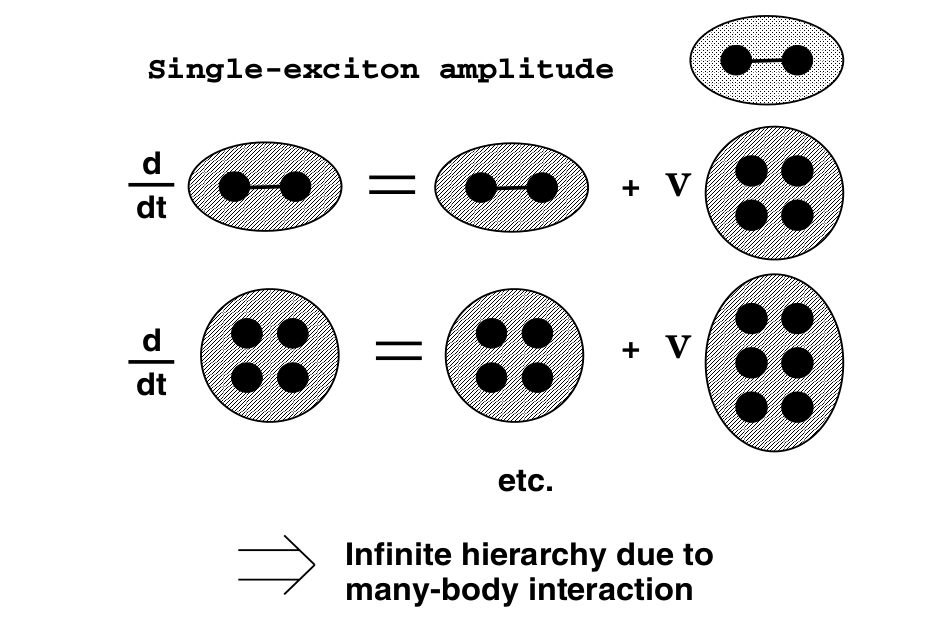
\includegraphics[width=0.70\textwidth]{./Figures/hatree-fock.png}
  %\rule{35em}{0.5pt}
  \caption[Hatree-Fock]{Phương trình chuyển động hữu hạn của hàm phân cực trong chất bán dẫn}
  \label{fig:Hatree-Fock}
  \end{figure}
  \begin{figure}[hc]
  \centering
  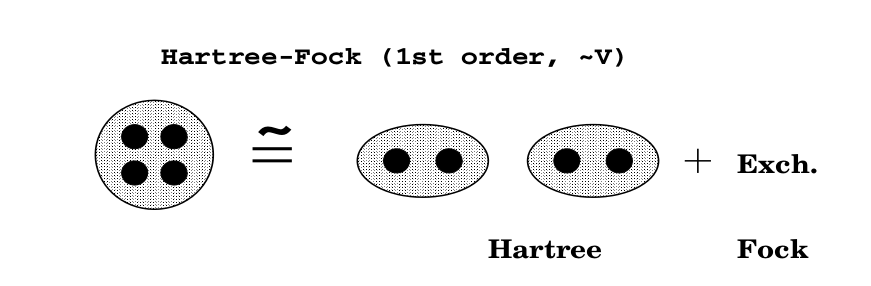
\includegraphics[width=0.70\textwidth]{./Figures/hatree-fock1.png}
  %\rule{35em}{0.5pt}
  \caption[Hatree-Fock]{Phương trình chuyển động được tính trong gần đúng Hatree-Fock Ref[19]}
  \label{fig:Hatree-Fock}
  \end{figure}
 Xét một ví dụ 
  \begin{align}
  \langle a_{k+q}^{\dagger}b_{-k}a_{k^{'}}a_{k+q}\rangle = \langle a_{k^{'}+q}^{\dagger}a_{k+q}\rangle\langle b_{-k}a_{k^{'}}\rangle - \langle a_{k^{'}+q}^{\dagger}a_{k^{'}}\rangle\langle b_{-k}a_{k+q}\rangle
  \end{align}
  và bây giờ ta giả sử $a_{k}^{\dagger}\propto e^{i\omega_k t}$ và $a_{k^{'}}\propto e^{-i\omega_{k^{'}} t}$ và ta có:
  \begin{equation}
  \langle a_{k}^{\dagger}a_{k^{'}}\rangle \propto e^{i(\omega_k -\omega_{k^{'}})}
  \end{equation}
  nó được biết đến như là phương pháp gần đúng pha ngẫu nhiên (Random Phase Approximation [1,15], ý tưởng gần đúng này cho rằng giá trị trung bình của các cặp toán tử $\langle a_{k}^{\dagger}a_{k^{'}}\rangle$ có sự phụ thuộc theo phase và thời gian như trên. Khi ta lấy tổng theo $k$ trị trung bình này thì chỉ có các số hạng chứa $k = k^{'}$ được giử lại, còn các số hạng khác do phase khác không nên bị dao động và trung bình theo thời gian đóng góp khác bằng không, với những lập luận ta viết lại biểu thức (2.36) như sau:
  \begin{align}
  \langle a_{k+q}^{\dagger}b_{-k}a_{k^{'}}a_{k+q}\rangle &= \langle a_{k^{'}+q}^{\dagger}a_{k+q}\rangle\langle b_{-k}a_{k^{'}}\rangle\delta_{kk^{'}} - \langle a_{k^{'}+q}^{\dagger}a_{k^{'}}\rangle\langle b_{-k}a_{k+q}\rangle\delta_{q,0}\notag \\
  &=n_{ek+q}p_k\delta_{k,k^{'}} - n_{ek^{'}}p_{k}\delta_{q,0}
  \end{align} 
  số hạng thứ 2 trong phương trình kia bị loại bỏ vì ta không xét trường hợp q=0

\chapter{\bfseries Lý Thuyết Cấu Trúc Vùng Năng Lượng Của Điện Tử Trong Bán Dẫn}
\label{Chapter2} % For referencing the chapter elsewhere, use \ref{Chapter1} 
Để hiểu được các tính chất quang học của chất bán dẫn, chẵn hạn như tính hấp thụ, khếch đại, dẫn điện, độ phân cực..., chúng ta cần phải biết cấu trúc vùng năng lượng, trong chương này ta sẽ thảo luận phương pháp tính toán cấu trúc vùng năng lượng của  một số chất bán dẫn, như chúng ta biết hầu hết các thiết bị quang học đều được cấu tạo từ các chất bán dẫn có vùng cấm là "thẳng" hay "trực tiếp", GaAs là chất như vậy, chất mà có đấy vùng dẫn và đỉnh của vùng hóa trị, nằm ở cùng một điểm trong vùng Brillouin, chất có đặt trưng như vậy sẽ rất thuận tiện nếu ta dùng phương pháp kp, sau đây ta sẽ nhắc lại một chút về định lý Bloch.
\section{Định lý Bloch}
Trong tinh thể lý tưởng, các ion dương sắp sếp một cách trật tự, tuần hoàn tại các nút mạng, các các điện tử hóa trị đồng vai trò là hạt tải điện được xem là chuyển động độc lập với nhau, trong một trường tuần hoàn được tạo bởi các ion dương, giả sử gọi $\mathit{l}$ là khoảng cách giữa các nút mạng lân cận, do tính chất đối xứng tịnh tiến của mạng tinh thể nên thế năng của điện tử trong tinh thể cũng có tính tuần hoàn tức:
\begin{equation}
\mathcal{T}_n V_0\left(\mathbf{r}\right) = V_0\left(\mathbf{r+\mathit{l}_n}\right) = V_0\left(\mathbf{r}\right)
\end{equation}
trong đó $\mathbf{\mathcal{T}_n}$ là toán tử tịnh tiến, $V_0\left(r\right)$ là thế năng hiệu dụng của điện tử do sự chồng chất của hạt nhân và các điện tử khác trong nguyên tử, như vậy Hamiltonian của điện tử trong nguyên tử có dạng sau:
\begin{equation}
\mathbf{\mathcal{H}_0} = \frac{\mathbf{p}^2}{2m_0} + \mathbf{V_0\left(\mathbf{r}\right)}
\end{equation}
cũng có tính chất tuần hoàn (đối xứng tịnh tiến) do ($\nabla_{r}^2 = \nabla_{r+l}^2$), biểu thức $(3.1)$ cho thấy các điểm $\mathbf{r}$ và $\mathbf{r+\mathit{l}}$ là tương đương với nhau về phương diện vật lý, do đó nếu đặt vào Hamiltonian $(2.2)$ tức ta thây $\mathbf{r}$ thành $\mathbf{r+\mathit{l}}$ thì hàm sóng điện tử ở vị trí $\mathbf{r}$  và $\mathbf{r+\mathit{l}}$ chỉ khác nhau một thừa số pha.
\begin{equation}
\mathcal{T}_n\psi\left(\mathbf{r}\right) = \psi\left(\mathbf{r+\mathit{l}_n}\right) = C_n\psi\left(\mathbf{r}\right)
\end{equation}
 Điều này có nghĩa là, khi dịch chuyển đi một véctơ tịnh tiến của mạng, do tính tuần hoàn của $V_0\left(\mathbf{r}\right)$, môđun của hàm sóng $\|\psi\left(\mathbf{r}\right)\|$ không đổi, chỉ có pha nó là thây đổi
 \begin{equation}
 \int\psi\left(\mathbf{r+l}\right)\psi^*\left(\mathbf{r+\mathit{l}}\right)dr = \|C_n\|^2  \int\psi\left(\mathbf{r}\right)\psi^*\left(\mathbf{r}\right)dr
 \end{equation}
Từ điều kiện chuẩn hóa của hàm sóng:
\begin{equation}
\int\psi\left(\mathbf{r}\right)\psi^*\left(\mathbf{r}\right)dr = 1     \Longrightarrow \|C_n\|^2 = 1
\end{equation}
Như vậy, $C_n$ hoặc phải bằng 1 hoặc bằng hàm số mũ với số mũ ảo. Vì hàm sóng biểu thị cho chuyển động của tinh thể, nên ở đây ta lấy $C_n$ là hàm mũ, số mũ có dạng sau [17].
\begin{equation}
C_n = e^{i\mathbf{k}\mathit{l}}
\end{equation}
trong đó $\mathbf{k}$ có thứ  nguyên trùng với thứ nguyên véctơ sóng (1/độ dài) nên ta cũng gọi nó là véctơ sóng, mỗi véctơ sóng  $\mathbf{k}$ khác nhau đặc trưng cho trạng thái của điện tử trong tinh thể(hay trong trường tuần hoàn). Chính xác ta nói  $\mathbf{k}$ là tập hợp 3 số lượng tử  đặc trưng cho trạng thái$\left(k_1,k_2,k_3\right)$. Giống như điện tử trong nguyên tử với bội 4 số lượng tử $\left(n,l,m,s\right)$ ta sẽ thấy điện tử trong tinh thể cũng có 4 số lượng tử $\left(k_x,k_y,k_z,s_z\right)$, do đó ta thêm chỉ số $\mathbf{k}$ vào hàm sóng của điện tử trong tinh thể:
\begin{equation}
\psi_k\left(\mathbf{r} + \mathit{l}\right) = e^{i\mathbf{r}\mathit{l}}\psi_k\left(\mathbf{r}\right)
\end{equation}
hay viết dưới dạng toán tử:
\begin{equation}
\mathcal{T}\psi_k\left(\mathbf{r}\right) = \psi_k\left(\mathbf{r}+\mathit{l}\right) = e^{i\mathbf{k}\mathit{l}}\psi_k\left(\mathbf{r}\right)
\end{equation}
biểu thức $(3.7)$ được biết đến như là một định lý Bloch.
Từ đây ta thấy rằng, hàm riêng của toán tử tịnh tiến $\mathcal{T}$ là $\psi\left(\mathbf{r}\right)$ và $e^{i\mathbf{k}\mathit{l}}$ là trị riêng tương ứng của hàm riêng đó.\\
Có thể chứng minh, toán tử Hamiltonian $\mathcal{H}$ và toán tử tịnh tiến $\mathcal{T}$ là giao hoán với nhau, do đó chúng có chung hệ hàm riêng, vì vậy hàm sóng của Hamiltonian của điện tử chuyển động trong tinh thể cũng thỏa mãn điều kiện tịnh tiến ở phương trình $(3.7)$, nhân 2 vế của $(3.7)$ với 
$e^{-i\mathbf{k}(\mathbf{r}+\mathit{l})}$ ta có:
\begin{equation}
e^{-i\mathbf{k}\left(\mathbf{r}+\mathit{l}\right)}\psi_k
\left(\mathbf{r}+\mathit{l}\right)
 = e^{-i\mathbf{kr}}e^{-i\mathbf{k}\mathit{l}}
 e^{i\mathbf{k}\mathit{l}}\psi_k\left(\mathbf{r}\right) =
  e^{-i\mathbf{kr}}\psi_k\left(\mathbf{r}\right)
\end{equation}
đặt:
\begin{gather}
u_k\left(\mathbf{r}\right) = e^{-i\mathbf{kr}}\psi_k\left(\mathbf{r}\right) \\
\Longrightarrow   u_k\left(\mathbf{r}+\mathit{l}\right) = 
e^{-i\mathbf{k}\left(\mathbf{r}+\mathit{l}\right)}
\psi_k\left(\mathbf{r}+\mathit{l}\right) =
e^{-i\mathbf{kr}}\psi_k\left(\mathbf{r}\right) = u_k\left(\mathbf{r}\right)
\end{gather}
từ $(3.10)$ ta có:
\begin{gather}
\psi_k\left(\mathbf{r}\right) = e^{i\mathbf{kr}}u_k\left(\mathbf{r}\right)
\end{gather}
trong đó
\begin{equation}
 u_k\left(\mathbf{r}+ \mathit{l}\right) = u_k\left(\mathbf{r}\right)
\end{equation}
Như vậy điện tử trong tinh thể được mô tả bởi sóng phẳng có biên độ biến đổi một cách tuần hoàn theo chu kỳ của trường tinh thể. Hàm $(3.12)$ được gọi là hàm Bloch. 

\section{Phương pháp kp}
   Để làm việc với phương pháp kp ta không quan tâm tới toàn bộ các dãi năng lượng, mà ta chỉ xét lân cận các cực trị của dãi năng lượng, theo sơ đồ dãi năng lượng $\mathbf{E}\left(\mathbf{k}\right)$ thì trong một dãy năng lượng $\mathbf{E}\left(\mathbf{k}\right)$ thay đổi theo $\mathbf{k}$ đạt cực đại rồi cực tiểu, thường thì ứng với $k_0=0$ năng lượng đạt cực trị nếu không ta phải tịnh tiến gốc để đạt được điều này, sau khi khảo sát tại điểm  $k_0$ ta mở rộng kết quả cho các trạng thái lân cận điểm  $k_0=0$, vậy ta có thể triển khai hàm sóng theo  $k_0=0$  như sau.
\begin{equation}
u_{m\mathbf{k}}\left(\mathbf{r}\right) = \sum_{n}a_{m\mathbf{k}}^nu_n\left(\mathbf{r}\right)
\end{equation}
trong đó $u_n\left(\mathbf{r}\right)$ thỏa mãn phương trình sau:
\begin{equation}
\left(\frac{p^2}{2m_0}+V_0(\mathbf{r}) \right)u_{n}(\mathbf{r}) = E_0u_{n}(\mathbf{r})
\end{equation}
thật vậy, xét tương tác của điện tử ở lân cận cực trị này bằng phương trình Schr$\ddot{o}$dinger:
\begin{equation}
\left(\frac{p^2}{2m_0}+V_0(\mathbf{r}) \right)\psi_{m\mathbf{k}}(\mathbf{r}) = E_{mk}\psi_{m\mathbf{k}}(\mathbf{r})
\end{equation}
ở đây: $m_0$ là khối lượng hiệu dụng của điện tử tụ do, $V_0$ thế dao dộng tuần hoàn, $m$ ở đây ta xem nó như là chỉ số đặc trưng của dãy năng lượng, $\mathbf{k}$ là véctơ sóng, 
thay $\psi_{m\mathbf{k}}$ ở phương trình $(3.12)$ vào$(3.16)$ ta có: \\
\begin{align}
&\left(\frac{p^2}{2m_0}+V_0(\mathbf{r}) + \frac{\hbar}{m_0}\mathbf{kp}+\frac{\hbar^2 k^2}{2m_0} \right)u_{m\mathbf{k}}(\mathbf{r}) = E_{mk}u_{m\mathbf{k}}(\mathbf{r})
\notag \\
&\Longleftrightarrow \left(\mathcal{H}_0 + \frac{\hbar}{m_0}\mathbf{kp}+\frac{\hbar^2 k^2}{2m_0}\right)u_{m\mathbf{k}}(\mathbf{r}) = E_{mk}u_{m\mathbf{k}}(\mathbf{r})
\end{align}

trong đó $\mathcal{H}_0$ thỏa mãn phương trinh $(3.15)$, để giải phương trình $(3.17)$ ta sử dụng lý thuyết nhiễu loạn không suy biến bậc 2 [23]:
\begin{equation}
\Longrightarrow E_{m\mathbf{k}}=E_{m0}+\frac{\hbar^2 k^2}{2m_0}+\frac{\hbar\mathbf{k}}{m_0}\langle m0|\mathbf{p} |m0\rangle +\frac{\hbar^2}{m_0}\sum_{m \ne n}\frac{{|\mathbf{k}\langle m0|\mathbf{p} |n0\rangle |}^2}{E_{m0}-E_{n0}}
\end{equation}
phương trình ở trên ta có thể viết lại dạng sau:
\begin{equation}
 E_{m\mathbf{k}}=E_{m0}+\frac{\hbar^2 k^2}{2m_0}+\frac{\hbar}{m_0}\mathbf{kp}_{mm} +\frac{\hbar^2}{m_0^2}\sum_{m \ne n}\frac{{|\mathbf{k}\mathbf{p}_{mn} |}^2}{E_{m0}-E_{n0}}
\end{equation}
trong đó:
\begin{equation}
\mathbf{p}_{mn}=\mathbf{p}_{mn}^\alpha=\int_{cell}\mathbf{u}_{m0}^*\mathbf{p}\mathbf{u}_{n0}\mathbf{dr}=
\int_{cell}\mathbf{u}_{m0}^*\left(\frac{h}{i}\nabla_\alpha \right)\mathbf{u}_{n0}\mathbf{dr}
\end{equation}
là mômen động lượng (có dạng ma trận) và có tính chất sau:
\begin{equation}
\mathbf{p}_{mm}^\alpha = 0;\mathbf{p}_{mn}^\alpha =\mathbf{p}_{nm}^\alpha = \left(\mathbf{p}_{mm}^\alpha \right)^*
\end{equation}
nếu ta xem điểm $k_0$ là điểm cực trị của hàm năng lượng $E_{n}\left(\mathbf{k}\right)$ thì ta có thể có được tính chất sau:
\begin{equation}
\mathbf{p}_{mn}^\alpha = \frac{m}{\hbar ^2}\left(\frac{\partial E_n\left(\mathbf{k}\right)}{\partial \mathbf{k}_\alpha}\right) = 0
\end{equation}
thây biểu thức $(3.21)$ và đồng thời viết lại biểu thức $(3.19)$ ta có kết quả sau:
\begin{equation}
 E_{m\mathbf{k}}=E_{m0}+\frac{\hbar^2 k^2}{2m_0} +\frac{\hbar^2}{m_0^2}\mathbf{k_\alpha}\mathbf{k_\beta}\sum_{m \ne n}\frac{{\mathbf{p}_{mn}^\alpha \mathbf{p}_{mn}^\beta }}{E_{m0}-E_{n0}}
\end{equation}
trong đó $\alpha,\beta=x,y,z$ là chỉ số Ensitanh, do đó ta có thể dẫn ra công thức sau:
\begin{equation}
\left(\frac{1}{m^*}\right)_{\alpha\beta}=\frac{1}{m_0}\delta_{\alpha\beta} +\frac{2}{m}\sum_{m \ne n}\frac{{\mathbf{p}_{mn}^\alpha \mathbf{p}_{mn}^\beta }}{E_{m0}-E_{n0}}
\end{equation}
Được gọi là tenso nghịch đảo của tenso khối lượng hiệu dụng do sự tương ứng với năng lượng cổ điển tự do, vậy công thức $(3.23)$ có thể viết lại như sau:
\begin{equation}
E_n\left(k\right) =E_0\left(k\right)+ \frac{\hbar^2}{2}\mathbf{k_\alpha}\mathbf{k_\beta}\left(\frac{1}{m^*}\right)_{\alpha\beta}
\end{equation} 
để tính bổ chính năng lương ta có nhận xét sau đây:
\begin{equation}
\langle \mathbf{u}_{m0}\left(\mathbf{r}\right)|\mathbf{p}|\mathbf{u}_{n0}\left(\mathbf{r}\right)\rangle \approx |\mathbf{p}| \approx \frac{\hbar}{a}
\end{equation}
\begin{equation}
\Longrightarrow \frac{1}{m^*} \approx \frac{1}{m}+\frac{2\hbar^2}{m^2a^2\Delta\epsilon}  \qquad \text{ với}\qquad \Delta\epsilon = E_{m0}-E_{n0}
\end{equation}

Hàm sóng của điện tử lúc này có dạng sau:
\begin{equation}
u_{mk}\left(\mathbf{r}\right) = u_{m0}\left(\mathbf{r}\right) + \left(\sum_{m\neq n}\frac{\hbar}{m_0}\frac{\mathbf{k}\mathbf{p}_{mn}^\alpha}{E_{m}-E_{n0}}\right)u_{n0}\left(\mathbf{r}\right) \equiv a_{mk}^nu_{nk}\left(\mathbf{r}\right)
\end{equation}
để ý chúng ta đã quay lại giả thiết ở biểu thức $(3.14)$, ở trên chúng ta chưa xét đến tương tác spin-orbit nếu chúng ta xét đến tương tác đó ta cần phải thêm số hạn sau:
\begin{equation}
\mathcal{H}_{SO} = \frac{\hbar}{4m^2_0}\boldsymbol{\sigma} \cdot \left(\boldsymbol{\nabla} V_0\times \boldsymbol{p} \right) =  \frac{\hbar}{4m^2_0}\left(\boldsymbol{\sigma}\times \boldsymbol{\nabla}V_0\right)\cdot\boldsymbol{p}
\end{equation}
trong đó $\boldsymbol{\sigma}$ là véctơ ma trận Pauli, và hàm sóng điện tử trong tinh thể thỏa mãn định lý Bloch
\begin{equation}
\psi_{m\mathbf{k}}(r) = e^{i\mathbf{kr}}u_{m\mathbf{k}}(\mathbf{r})
\end{equation}
với $u_{m\mathbf{k}}(\mathbf{r})$ là hàm tuần hoàn theo chu kỳ tinh thể, và hàm Bloch có tính chất sau đây.
\begin{align}
\left \langle\psi_{m\mathbf{k}}\Bigl\vert\psi_{m'\mathbf{k}'}\right \rangle &\equiv \int d\mathcal{V}\psi_{m\mathbf{k}}^*(\mathbf{r})\psi_{m'\mathbf{k}'}(\mathbf{r}) = \delta_{mm'}\delta\left(\boldsymbol{k-k'}\right) \\
\left \langle u_{m\mathbf{k}}\Bigl\vert u_{m'\mathbf{k}'}\right \rangle &\equiv \int d\Omega u_{m\mathbf{k}}^* u_{m'\mathbf{k}'} = \delta_{mm'}\frac{\Omega}{\left(2\pi \right)^3}
\end{align}
ở đây $V\left(\Omega\right)$ là thể tích chuẩn hóa của tinh thể(unit-cell). Hamiltonian của hệ lúc này có dạng tổng quát như sau:
\[H=\mathcal{H}_0 +\mathcal{H}_{SO}\]
lặp lại các phép tính tương tự như trên, chúng ta có kết quả tương tự nhưng chỉ khác nhau ở một chỗ là thành phần động lượng $p_{mn}^\alpha$ lúc này có dạng như sau $\pi_{mn}$:
\begin{equation}
\boldsymbol{\pi_{mn}}=\int_{cell} u_{m0}^*\left( \frac{\hbar}{i}\nabla_\alpha + \frac{1}{4m_0c^2} \left(\boldsymbol {\sigma}\times\boldsymbol{ \nabla} V\right)\right)u_{n0}d\mathbf{r}
\end{equation} 
còn năng lượng của nó có dạng sau:
\begin{equation}
 E_{m\mathbf{k}}=E_{m0}+\frac{\hbar^2 k^2}{2m_0}+\frac{\hbar}{m_0}\mathbf{k}\boldsymbol{\pi}_{mm} +\frac{\hbar^2}{m_0^2}\sum_{m \ne n}\frac{{\Bigl\vert\mathbf{k}\boldsymbol{\pi}_{mn} \Bigr\vert}^2}{E_{m0}-E_{n0}}
\end{equation}
cần chú ý rằng ta có thể chứng minh $[11]$:
\begin{equation}
\boldsymbol{\pi}_{mm}^\alpha=\boldsymbol{\pi}_{mm}= \frac{m}{\hbar^2}\left(\frac{\partial E_m\left(k\right)}{\partial \mathbf{k}_\alpha}\right)_0
\end{equation}
nếu ta xét điểm $k_\alpha$ là điểm cực trị thì $\boldsymbol{\pi_{mn}}=0$, do đó ta viết biểu thức $(3.34)$ lại như sau:
\begin{equation}
 E_{m\mathbf{k}}=E_{m0}+\frac{\hbar^2 k^2}{2m_0} +\frac{\hbar^2}{m_0^2}\sum_{m \ne n}\frac{{\Bigl\vert\mathbf{k}\boldsymbol{\pi}_{mn}\Bigl\vert}^2}{E_{m0}-E_{n0}}=E_{m0}+\frac{\hbar^2}{m_0}\mathbf{k_\alpha}\mathbf{k_\beta}\left(\frac{1}{m^*}\right)_{\alpha\beta}
\end{equation}

\section{Mô hình kp 2 vùng,kp 4 vùng}
\subsection{Mô hình kp 2 vùng}
Theo $(3.28)$ ta có thể viết hàm sóng điện tử như sau: 
\begin{equation}
u_{m\mathbf{k}}\left(\mathbf{r}\right) = \sum_n a_{m\mathbf{k}}^nu_{n0}\left(\mathbf{r}\right)
\end{equation}

thây biểu thức trên vào $(3.17)$ và nhân $u_{n0}^*$ vào bên trái của 2 vế, đồng thời lấy tích phân và chuẩn hóa hàm sóng ta có kết quả sau:
\begin{equation}
\mathlarger{\sum_{n'}} \mathsmaller{\left[  \left(E_{n0}+\frac{\hbar^2 k^2}{2m_0}\right)\delta_{nn'}  +\frac{\hbar}{m_0}\mathbf{k}\mathbf{p}_{nn'}\right]a_{m\mathbf{k}}^{n'}}
=E_{mk}a_{m\mathbf{k}}^n
\end{equation}
chú ý rằng ở đây ta đã sử dụng tính chất $\int u_{n0}^*u_{n'0}d\mathbf{r}=\delta_{nn'}$. Để tìm năng lượng của điện tử, ta  giải phương trình trên tức ta đi tính định thức sau:
 \begin{equation}
 \begin{Vmatrix}
 E_{n0}+\frac{\hbar^2 k^2}{2m_0} -E       & \frac{\hbar}{m_0}\mathbf{k}\mathbf{p}_{nn'} \\
 \frac{\hbar}{m_0}\mathbf{k}\mathbf{p}_{n'n}    & E_{n'0}+\frac{\hbar^2 k^2}{2m_0} -E 
 \end{Vmatrix} =0
 \end{equation}
 sau vài bước tính toán ta có kết quả sau:
 \begin{equation}
 E = \frac{1}{2}\left[ E_n+E_{n'}+\frac{\hbar^2}{m_0}k^2\right] \pm \left[\frac{1}{2}\left(E_n-E_{n'}\right)^2+\frac{4\hbar^2}{m_0^2}|kp|^2\right]^{1/2}
\end{equation} 
 Bây giờ ta xét 2 dãy năng lượng, dãy thứ nhất tương ứng vùng dẫn $\left(n=c\right)$ và dãy thứ 2 tương ứng với vùng hóa trị $\left(n'=v\right)$, giả sử ta chọn điểm $\mathbf{k}_0=0 $ \emph{sao cho} $E_v=0\Longrightarrow E_c=E_g$
vậy ta có thể viết lại định thức trên như sau:
  \begin{equation}
 \begin{Vmatrix}
 E_{c}+\frac{\hbar^2 k^2}{2m_0} -E       & \frac{\hbar}{m_0}\mathbf{k}\mathbf{p}_{cv} \\
 \frac{\hbar}{m_0}\mathbf{k}\mathbf{p}_{vc}    & E_{v}+\frac{\hbar^2 k^2}{2m_0} -E 
 \end{Vmatrix} =0
 \end{equation}
 và năng lượng của điện tử là:
 \begin{equation}
 E = \frac{1}{2}\left(E_g+\frac{\hbar^2 k^2}{m_0} \right) \pm \frac{1}{2}\left[ E_g^2 +4\frac{\hbar^2}{m_0^2}|kp|^2\right]^{1/2}
 \end{equation}
xét trường hợp $kp_{cv}$  rất nhỏ ta có:
\begin{equation}
E=\left\{
 \begin{array}{cc}
E_g+\frac{\hbar^2 k^2}{2m_0}+\frac{\hbar^2}{E_gm_0^2}|kp_{cv}|^2 \qquad \text{vùng dẫn} \\
\frac{\hbar^2 k^2}{2m_0}-\frac{\hbar^2}{E_g m_0^2}|kp_{cv}|^2 \qquad \qquad \text{vùng hóa trị}
 \end{array} \right.
\end{equation}
và ta giả sử $p_{cv}$ là đẳng hướng vì vậy ta có $\vec{k}\vec{p}_{cv}=kp_{cv}$, vì vậy ta có thể suy ra khối lượng hiệu dụng ở vùng hóa trị và vùng dẫn như sau:
\begin{equation}
\Longrightarrow\left\{
\begin{array}{cc}
\frac{1}{m_v^*}&=\frac{1}{m_0}-\frac{2p_{cv}^2}{E_g}\\
\frac{1}{m_c^*}&=\frac{1}{m_0}+\frac{2p_{cv}^2}{E_g}
\end{array} \right.
\end{equation}
 
 \subsection{Mô hình kp 4 vùng}
Để thấy rõ hơn ta xét trường hợp mô hình 4 vùng, trước hết để đơn giản ta bỏ qua trường hợp có tương tác spin-orbit, và xét 1 dãy dẫn và 3 dãy hóa trị .
 \begin{itemize}
 \item [a.] 1 dãy dân tương ứng với năng lượng $E_s$ 
 \item [b.] 3 dãy hóa trị tương ứng với năng lượng $E_p$
 \end{itemize}
 và ta xét tại điểm $k_0=0$ ta có:
 \begin{align}
 &\mathcal{H}_0u_{s0}(\mathbf{r}) = E_s^0u_{s0}(\mathbf{r}),
 \mathcal{H}_0u_{p_x0}(\mathbf{r}) = E_{p_x}^0u_{p_x0}(\mathbf{r}) \notag  \\
 &\mathcal{H}_0u_{p_y0}(\mathbf{r}) = E_{p_y}^0u_{p_y0}(\mathbf{r}),
 \mathcal{H}_0u_{p_z0}(\mathbf{r}) = E_{p_z}^0u_{p_z0}(\mathbf{r})
\end{align}  
khi $k\neq 0$ theo $(3.14)$ ta có thể mở rộng hàm sóng điện tử lận cận điểm $k \neq 0$. Sử dụng các công thức ở trên và tính toán tương tự ta dẫn ra được ma trận sau đây:
\begin{equation}
u_{m\mathbf{k}}(\mathbf{r})=\sum_n a_{m\mathbf{k}}^n u_{n0}(\mathbf{r}) \qquad m=1,2,3,4,n \in {s,p_x,p_y,p_z}
\end{equation} 

\begin{equation}
\begin{pmatrix}
E_s^0+\frac{\hbar^2 k^2}{2m_0} & \frac{\hbar}{m_0}k_xp & \frac{\hbar}{m_0}k_yp & \frac{\hbar}{m_0}k_zp \\
\frac{\hbar}{m_0}k_xp^* & E_p^0+\frac{\hbar^2 k^2}{2m} & 0 & 0 \\
\frac{\hbar}{m_0}k_yp^* & 0 & E_p^0+\frac{\hbar^2 k^2}{2m}  & 0 \\
\frac{\hbar}{m_0}k_zp^* & 0 &0 & E_p^0+\frac{\hbar^2 k^2}{2m}  
\end{pmatrix}
\begin{pmatrix}
a_{1k}^s \\
 a_{2k}^{p_x} \\
  a_{3k}^{p_y} \\
   a_{4k}^{p_z}
\end{pmatrix}
=E_{mk}\begin{pmatrix}
a_{1k}^s \\
 a_{2k}^{p_x} \\
  a_{3k}^{p_y} \\
   a_{4k}^{p_z}
\end{pmatrix}
\end{equation}
để tính năng lượng của điện tử ta giải phương trình trên, ta sử dụng phần mềm Mapple ta tính được kết quả sau:
\begin{align}
&\left[\left(E_{mk} -\frac{\hbar^2 k^2}{2m_0}\right)^2 - (E_{mk}-\frac{\hbar^2}{2m_0})(E_s^0+E_p^0)+E_p^0E_p^0 -\left(\frac{\hbar}{m}\mathbf{k}|p|\right)^2 \right]\notag \\
&\times \left(E_{mk} -\frac{\hbar^2 k^2}{2m_0 -E_p^0} \right)^2 =0
\end{align}
vì vậy ta có thể có năng lượng ở các dãy như sau:
\begin{align}
E_{m\mathbf{k}}=&E_s^0 +\frac{\hbar^2 k^2}{2m_0},\notag \\
E_{m\mathbf{k}}=&\frac{E_s^0 +E_p^0}{2} \pm \sqrt{\left(\frac{E_s^0 +E_p^0}{2}\right)^2 +\left(\frac{\hbar}{m_0}\mathbf{k}|p|\right)^2}+\frac{\hbar^2 k^2}{2m_0}
\end{align}
Bây giờ ta xét đến số hạng  tương tác spin-orbit:
\begin{equation}
\mathcal{H}_{SO} = \frac{\hbar}{4m^2_0}\boldsymbol{\sigma} \cdot \left(\boldsymbol{\nabla} V_0\times \boldsymbol{p} \right) =  \frac{\hbar}{4m^2_0}\left(\boldsymbol{\sigma}\times \boldsymbol{\nabla}V_0\right)\cdot\boldsymbol{p}
\end{equation}
phương trình Schr$\ddot{o}$dinger lúc này có dạng sau:
\begin{equation}
\left[\mathcal{H}_0+\frac{{\hbar}^2k^2}{2m_0}+\frac{\hbar}{m_0}\boldsymbol{k}\left(\boldsymbol{p}+\frac{\hbar}{4m^2_0}\boldsymbol{\sigma}\times\boldsymbol{\nabla} V_0 \right)+\frac{\hbar}{4m^2_0}\boldsymbol{\sigma}\left(\boldsymbol{\nabla} V_0\times \boldsymbol{p} \right)\right]u_{m\mathbf{k}}(\mathbf{r}) = E_{m\mathbf{k}}u_{m\mathbf{k}}(\mathbf{r})
\end{equation}
ở biểu thức trên ta cần chú ý rằng do vận tốc quỹ đạo của điện tử rất là lớn so với vận tốc của  một hàm sóng lân cận điểm $k_0$, nói cách khác mômen động lượng của nguyên tử trong tinh thể là rất nhỏ so với mômen động lượng của điện tử  quay quanh nguyên tử ta viết lại biểu thức ở trên như sau:
\begin{equation}
\Longrightarrow \mathcal{H}u_{m\mathbf{k}}(\mathbf{r}) \approx \left(\mathcal{H}_0 +\frac{\hbar^2 k^2}{2m_0}+\frac{\hbar}{m_0}\mathbf{kp}+ \frac{\hbar}{4m^2_0}\boldsymbol{\sigma}\left(\boldsymbol{\nabla} V_0\times \boldsymbol{p} \right)\right)u_{m\mathbf{k}}(\mathbf{r})=E_{m\mathbf{k}}u_{m\mathbf{k}}(\mathbf{r})
\end{equation}  
\subsubsection{Phân tích hàm sóng cơ sở và thành phận ma trận Hamiltonian}
\begin{itemize}
\item[-] Ta viết lại 
\begin{equation}
u_{m\mathbf{k}}(\mathbf{r})= \sum_n a_{mk}^n u_{n0}(\mathbf{r})
\end{equation}
\item[-] Vùng dẫn:$\left| S\Bigl\uparrow \right\rangle,\left| S\Bigl\downarrow\right\rangle \qquad \text{với năng lượng}:E_s$

\item[-] Vùng hóa trị:$\left| X\Bigl\uparrow\right\rangle,\left| Y\Bigl\uparrow\right\rangle,
\left |Z\Bigl\uparrow\right\rangle,
\left|X\Bigl\downarrow\right\rangle,
\left|Y\Bigl\downarrow\right\rangle,
\left|Z\Bigl\downarrow\right\rangle \qquad \text{với năng lượng}:E_p
$
\end{itemize}
trong đó:$\mathcal{H}_0\left|S\Bigl\uparrow\right\rangle=E_s\left|S\Bigl\uparrow\right\rangle,\mathcal{H}_0\left|S\Bigl\downarrow\right\rangle=E_s\left|S\Bigl\downarrow\right\rangle,\mathcal{H}_0\left|X\Bigl\uparrow\right\rangle=E_p\left|X\Bigl\uparrow\right\rangle,\mathcal{H}_0\left|X\Bigl\downarrow\right\rangle=E_p\left|X\Bigl\downarrow\right\rangle \ldots$
có nhiều cách khác nhau để chọn hàm sóng cơ sở $u_{n0}(\mathbf{r})$ nhưng để cho thuận lợi cho việc tính toán ma trận Hamiltonian, ta chọn hàm sóng $u_{n0}(\mathbf{r})$ như sau [23,9,24]:
\begin{align}
|u_1\rangle =|S\downarrow\rangle, |u_2\rangle=\left |\frac{X-iY}{\sqrt{2}}\Bigl\uparrow \right\rangle, |u_3\rangle= \left |Z\downarrow \right\rangle, |u_4\rangle =-\left |\frac{X+iY}{\sqrt{2}}\Bigl\uparrow \right\rangle 
\end{align}
\begin{equation}
|u_5\rangle = |S\uparrow\rangle, |u_6\rangle=-\left|\frac{X+iY}{\sqrt{2}}\Bigl\downarrow\right\rangle, |u_7\rangle=\left |Z\uparrow\right\rangle, u_8\rangle=\left |\frac{X-iY}{\sqrt{2}}\Bigl\downarrow\right\rangle
\end{equation}
ở đây$|S\rangle=S(\mathbf{r}),|X\rangle=xf(\mathbf{r}),|Y\rangle=yf(\mathbf{r})$, xét nếu \emph{x} lẽ $\rightarrow \emph{f(x)} $ phải chẳn, tức $X(x,y,z)=-X(-x,y,z)$,
 ma trận Pauli
\begin{equation}
\delta_x=\begin{bmatrix}
0 & 1 \\
1 & 0
\end{bmatrix}
\delta_y=\begin{bmatrix}
0 & -i \\
i & 0
\end{bmatrix}
\delta_z=\begin{bmatrix}
1 & 0 \\
0 & -1
\end{bmatrix}
\end{equation}
spin up: $|\uparrow\rangle=\begin{bmatrix}
1 \\ 0
\end{bmatrix}$ và spin down:$|\downarrow\rangle=\begin{bmatrix}
0 \\1
\end{bmatrix}$ và ta có tính chất sau$\langle\uparrow|\uparrow\rangle=\langle\downarrow|\downarrow\rangle=1,\langle\uparrow|\downarrow\rangle=\langle\downarrow|\uparrow\rangle=0$ \\
Sau đây ta sẽ tính toán vài thành phần ma trận trong Hamiltonian: 
\begin{align*}
\mathcal{H}_{11}&=\Bigl\langle u_1\Bigl\vert H \Bigr\vert u_1\Bigr\rangle =
\Bigl\langle S\Bigl \downarrow\Bigl\vert \mathcal{H}_0 + \frac{\hbar^2 k^2}{2m_0} +\frac{\hbar}{m}\mathbf{kp}+\frac{\hbar}{4m_0^2c^2}\sigma\cdot\nabla V\times p \Bigr\vert S\Bigr\downarrow \Bigr\rangle  \\
&=\Bigl\langle S\Bigl\downarrow \Bigl\vert \mathcal{H}_0+\frac{\hbar^2 k^2}{2m_0}\Bigr\vert S\Bigr\downarrow \Bigr\rangle +
\Bigl\langle S\Bigl\downarrow\frac{\hbar}{m}\mathbf{kp} \Bigr\vert S\Bigr\downarrow\Bigr\rangle +
\Bigl\langle S\Bigl\downarrow \Bigr\vert \frac{\hbar}{4m_0^2c^2}\sigma\cdot\nabla V\times \mathbf{p}\Bigr\vert S\Bigr\downarrow \Bigr\rangle
\end{align*}

xét $\langle S\downarrow |p|S\downarrow\rangle=\langle S|p|S\rangle=\int S(\mathbf{r})\frac{\hbar}{i}\nabla S(\mathbf{r})\mathbf{dr} =0$\\
và $\sigma(\nabla V\times \mathbf{p})=\sigma_x(\nabla V\times p)_x+\sigma_y(\nabla V\times p)_y+\sigma_z(\nabla V\times p)_z$;
mà $\langle\downarrow|\sigma_x|\downarrow\rangle=\langle\downarrow|\sigma_x|\downarrow\rangle=0$

\begin{equation}
\Longrightarrow \mathcal{H}_{11}= E_s^0 +\frac{\hbar^2 k^2}{2m_0}+\Bigl\langle S\Bigl\vert(\nabla V\times \mathbf{p})_z\Bigr\vert S\Bigr\rangle=E_s^0 +\frac{\hbar^2 k^2}{2m_0} 
\end{equation}

\begin{align*}
\mathcal{H}_{13}=\Bigl\langle u_1\Bigl\vert H \Bigr\vert u_3\Bigr\rangle  &=\Bigl\langle S\Bigl\downarrow \Bigl\vert \mathcal{H}_0+\frac{\hbar^2 k^2}{2m_0} +\frac{\hbar}{m}\mathbf{kp}+\frac{\hbar}{4m_0^2c^2}\sigma\cdot\nabla V\times p \Bigr\vert Z\Bigr\downarrow \Bigr\rangle \\
&=\Bigl\langle S\Bigl\downarrow \Bigl\vert \mathcal{H}_0+\frac{\hbar^2 k^2}{2m_0}\Bigr\vert Z\Bigr\downarrow\Bigr\rangle + \Bigl\langle S\Bigl\downarrow\frac{\hbar}{m}\mathbf{kp}\Bigr\vert Z\Bigr\downarrow\Bigr\rangle + \Bigl\langle S\Bigl\downarrow\Bigl\vert \frac{\hbar}{4m_0^2c^2}\sigma\cdot\nabla V\times \mathbf{p} \Bigr\vert Z\Bigr\downarrow\Bigr\rangle\\
&=0 -\frac{\hbar}{m_0}\mathbf{k}_z\Bigl\langle S\Bigl\vert\mathbf{p}_z\Bigr\vert Z\Bigr\rangle + 0=-\mathbf{k}\mathbf{P}
\end{align*}
ở đây ta đã định nghĩa $\mathbf{P}=-\frac{\hbar}{m_0}\langle S|\mathbf{p}_z|Z\rangle$
\begin{align*}
\mathcal{H}_{22}=\Bigl\langle u_2\Bigl\vert H \Bigr\vert u_2\Bigr\rangle &=\frac{1}{\sqrt{2}}\Bigl\langle (X+iY)\Bigl\uparrow\Bigl\vert \mathcal{H}_0+\frac{\hbar^2 k^2}{2m_0} +\frac{\hbar}{m}\mathbf{kp}+\frac{\hbar}{4m_0^2c^2}\sigma\cdot\nabla V\times p \Bigr\vert(X-iY)\Bigr\uparrow\Bigr\rangle \frac{1}{\sqrt{2}}  \\
&=E_p^0 +\frac{\hbar^2 k^2}{2m_0}- \frac{\Delta}{3}
\end{align*}
ở đây ta định nghĩa $\Delta=\frac{3i\hbar}{4m_0^2c^2}\langle X|(\nabla V\times p)_z|Y\rangle$, các hệ số còn lại ta tính tương tự, sau khi tính toán song ta có một ma trận sau:
\begin{equation}
\mathcal{H}_{88}=\begin{bmatrix}
\overline{H} &0 \\
0 & \overline{H}
\end{bmatrix} \text{với} \qquad \overline{H}
\end{equation}
\begin{equation}
\overline{H}=
\begin{bmatrix}
E_s^0  &0 &\mathbf{kP}  &0 \\
0& E_p^0 -\frac{\Delta}{3} &\sqrt{2}\frac{\Delta}{3} &0 \\
\mathbf{kP} &\sqrt{2}\frac{\Delta}{3} &E_p^0 &0 \\
0 &0 &0 &E_p^0+\frac{\Delta}{3} 
\end{bmatrix}
\end{equation}
ta định nghĩa $E_s^0=E_g;E_p^0=-\frac{\Delta}{3}$,phương trình $(3.59)$ trở thành như sau:
\begin{equation}
\overline{H}=
\begin{bmatrix}
E_g  &0 &\mathbf{kP}  &0 \\
0 &-2\frac{\Delta}{3} &\sqrt{2}\frac{\Delta}{3} &0 \\
\mathbf{kP} &\sqrt{2}\frac{\Delta}{3} &-\frac{\Delta}{3} &0 \\
0 &0 &0 &0 
\end{bmatrix}
\end{equation}
ta tính định thức sau $det|\overline{H}-E'I|=0$,ở đây $E'=E+\frac{\hbar^2 k^2}{2m_0}$ đó cũng là lý do ta không thấy hệ số này ở trên ma trận, giải định thức trên cho ta 4 trị riêng năng lượng:
\begin{enumerate}
\item \begin{equation}
E'=0 \qquad \text{(năng lượng $E_g$ là bằng 0)}
\end{equation}
\item \begin{equation}
E'(E'-E_g)(E'+\Delta) -k^2P^2(E'+2\Delta /3) =0
\end{equation}
phương trình trên ta xét, trường hợp $k=0 \Longrightarrow $ có 3 dãy,$E'=0,E'=E_g$ và $E'=-\Delta$, và ta xét trường hợp $k\approx0$ tức $\epsilon(k) \ll \Delta,E_g$
\begin{itemize}
\item[(i)] với $E'=E_g + \epsilon(k^2)$ thay vào phương trình $(3.62)$ ta có:
\begin{equation}
\epsilon(k) \simeq \frac{k^2P^2(E_g+2\Delta /3)}{E_g(E_s+\Delta)}
\end{equation}
\item[(ii)] với $E'=0+\epsilon(k^2)$ thay vào phương trình $(3.62)$ ta có:
\begin{equation}
\epsilon(k) \simeq \frac{-2k^2P^2}{3E_g}
\end{equation}
\item[(iii)] với $E'=-\Delta+\epsilon(k^2)$ thay vào phương trình $(3.62)$ ta có:
\begin{equation}
\epsilon(k) \simeq \frac{-k^2P^2}{3(E_g+\Delta)}
\end{equation}

\end{itemize}
\end{enumerate}
Vì $E'=E+\frac{\hbar^2 k^2}{2m_0}$ nên ta thây nó vào các phương trình $(3.63),(3.65)-(3.67)$ ta có:
\begin{align}
(3.63)&\qquad n=c \Longrightarrow E_c(\mathbf{k})=E_s^0 +\frac{\hbar^2 k^2}{2m_0}+ \frac{k^2P^2(E_g+2\Delta /3)}{E_g(E_s+\Delta)}\\
(3.61)&\qquad n=hh \Longrightarrow E_{hh}(\mathbf{k})=\frac{\hbar^2 k^2}{2m_0}\\
(3.64)&\qquad n=lh \Longrightarrow E_{lh}(\mathbf{k})=\frac{\hbar^2 k^2}{2m_0}-\frac{k^2P^2}{3E_g}\\
(3.65)&\qquad n=so \Longrightarrow E_{so}(\mathbf{k})=-\Delta +\frac{\hbar^2 k^2}{2m_0}-\frac{k^2P^2}{3(E_g+\Delta)}
\end{align}
Chú ý rằng kết quả trên đây là không đầy đủ cho lắm, vì các hiệu ứng ở các band ở trên ta chưa tính vào, ta sẽ thảo luận nó trong phần \emph{mô hình Kane mở rộng và lý thuyết nhiễu loạn L$\ddot{o}$win} và phần năng lượng ở \emph{heavy-hole} là sai ta sẽ sửa lại ở phần sau, do đó ta cần phải chọn hàm cơ sở sao cho khi tính toán năng lượng ở lỗ trống nhẹ có kết quả là âm, vì vậy ta cần phải chọn hàm sóng (riêng) lại, do đó từ phương trình $(3.60)$ ta có thể chọn hàm riêng như sau cho ma trận $4\times 4$ của thành phần thứ nhất trong $(3.62)$:
\begin{align*}
&\phi_{hh,\alpha}=\left |-\left(\frac{X+iY}{\sqrt{2}}\right)\Bigl\uparrow\right\rangle \qquad \qquad\text{hh band}\\
&\phi_{n,\alpha}=a_n\left | S\Bigl\downarrow\right\rangle +b_n\left |\left(\frac{X-iY}{\sqrt{2}}\right)\Bigl\uparrow\right\rangle +c_n\left |Z\Bigl\downarrow\right\rangle \qquad \text{n=c,lh,so}
\end{align*}
và thành phần thứ 2 ma trận $4\times4$ trong phương trình $(3.62)$
\begin{align*}
&\phi_{hh,\alpha}=\left |\left(\frac{X-iY}{\sqrt{2}}\right)\Bigl\downarrow\right\rangle \qquad \qquad\text{hh band}\\
&\phi_{n,\alpha}=a_n\left |S\Bigl\uparrow\right\rangle +b_n\left |-\left(\frac{X+iY}{\sqrt{2}}\right)\Bigl\downarrow\right\rangle +c_n\left |Z\Bigl\uparrow\right\rangle \qquad \text{n=c,lh,so}
\end{align*}
do đó ta tìm  trị riên năng lượng và chuẩn hóa lại trị véctơ của phương trình $(3.64):$
\begin{equation}
\begin{bmatrix}
E_g -E_n' &0 &\mathbf{kP}  \\
0 &\frac{-2\Delta}{3}-E_n' &\frac{\sqrt{2}\Delta}{3} \\
\mathbf{kP} &\sqrt{2}\frac{\Delta}{3} &-\frac{\Delta}{3}-E_n' \\
\end{bmatrix}
\begin{bmatrix}
a_n \\b_n \\c_n
\end{bmatrix}
=0
\end{equation}
sau khi giải phương trình trên ta tìm được trị riêng của năng lượng, sau đó ta chuẩn hóa trị riêng của véctơ ta có [9,23], $(a_n^2+b_n^2 +c_n^2)^{1/2}=1$, đồng thời xét trường hợp  $k^2\rightarrow 0$:
\begin{align*}
n&=c \qquad a_n\approx 1 \qquad b_n\approx 0, \qquad c_n\approx 0 \\
n&=lh \qquad a_n\approx 0 \qquad b_n = \frac{1}{\sqrt{3}}, \qquad c_n = \sqrt{\frac{2}{3}} \\
n&=c \qquad a_n\approx 0 \qquad b_n =  \sqrt{\frac{2}{3}}, \qquad c_n = -\frac{1}{3} 
\end{align*}
thây các hệ số này vào các hàm riêng ở phương trình trên ta có hàm riêng ta mong muốn, thật ra nếu ta áp dụng lý thuyết về gốc mômen động lượng(Theory of angular momentum) [9] ta cũng có kết quả tương tự:
\begin{align*}
&\left |\frac{3}{2},\frac{3}{2}\right\rangle =\left |1,\frac{1}{2};1,+\right\rangle \\
&\left |\frac{3}{2},\frac{1}{2}\right\rangle =\sqrt{\frac{2}{3}}\left |1,\frac{1}{2};0,+\right\rangle +\frac{1}{\sqrt{3}}\left |1,\frac{1}{2},1,-\right\rangle \\
&\left |\frac{3}{2},-\frac{1}{2}\right\rangle = \frac{1}{3}\left |1,\frac{1}{2};-1,+\right\rangle +\sqrt{\frac{2}{3}}\left |1,\frac{1}{2},0,- \right\rangle \\
&\left |\frac{3}{2},-\frac{3}{2}\right\rangle = \left |1,\frac{1}{2};-1,-\right\rangle
 \end{align*}
 và:
 \begin{align*}
&\left |\frac{1}{2},\frac{1}{2}\right\rangle = \sqrt{\frac{2}{3}}\left |1,\frac{1}{2};1,-\right\rangle -\frac{1}{\sqrt{3}}\left |1,\frac{1}{2},0,+\right\rangle \\
&\left |\frac{1}{2},-\frac{1}{2}\right\rangle = \frac{1}{3}\left |1,\frac{1}{2};0,-\right\rangle -\sqrt{\frac{2}{3}}\left |1,\frac{1}{2},-1,+\right\rangle 
\end{align*}  
\subsubsection{Tóm tắt kết quả mô hình kp 4 vùng như sau:}
Tôi tóm tắt kết quả ở dưới đây: 
\begin{enumerate}
\item vùng dẫn
\begin{align*}
E_c(\mathbf{k})&=E_s^0 +\frac{\hbar^2 k^2}{2m_0}+ \frac{k^2P^2(E_g+2\Delta /3)}{E_g(E_s+\Delta)}\left(\equiv   E_g+\frac{\hbar^2 k^2}{2m_e^*}\right)\\
\phi_{c\alpha}&=\left |S\Bigl\uparrow \right\rangle \\
\phi_{c\beta}&=\left |S\Bigl\downarrow \right\rangle
\end{align*}
\item vùng hóa trị
\begin{itemize}
\item[a/]  Heavy hole
\begin{align*}
E_{hh}(\mathbf{k})&=\frac{\hbar^2 k^2}{2m_0}\left(\text{cần có dạng } \qquad  -\frac{\hbar^2 k^2}{2m_{hh}^*}\right)\\
\phi_{hh,\alpha}&=\frac{-1}{\sqrt{2}} \left |(X+iY)\Bigl\uparrow \right\rangle \equiv \left |\frac{3}{2},\frac{-3}{2}\right\rangle \\
\phi_{hh,\beta}&=\frac{1}{\sqrt{2}}\left |(X-iY)\Bigl\downarrow \right\rangle \equiv \left |\frac{3}{2},\frac{3}{2}\right\rangle 
\end{align*}
\item[b/] light hole
\begin{align*}
E_{lh}(\mathbf{k})&=\frac{\hbar^2 k^2}{2m_0}-\frac{2k^2P^2}{3E_g}\left(\equiv -\frac{\hbar^2 k^2}{2m_{lh}^*}\right)\\
\phi_{lh,\alpha}&=\frac{-1}{\sqrt{2}} \left |(X+iY)\Bigl\uparrow\right\rangle
\equiv \left |\frac{3}{2},\frac{-3}{2}\right\rangle \\
\phi_{lh,\beta}&=\frac{1}{\sqrt{2}}\left |(X-iY)\Bigl\downarrow\right(\rangle 
\equiv \left |\frac{3}{2},\frac{3}{2}\right\rangle 
\end{align*}
\end{itemize}
\end{enumerate}

\newpage

\chapter{\bfseries Mô Hình Kane Mở Rộng và Lý Thuyết Nhiễu Loạn $\mathbf{L\ddot{o}wdin}$}
\label{Chapter3} % For referencing the chapter elsewhere, use \ref{Chapter1} 
Cho tới lúc này chúng ta đã tính được gần đúng cấu trúc vùng năng lượng của chất bán dẫn, nhưng để có độ chính xác cao  ta sẽ kết hợp phương pháp kp với gần đúng là 14-band , ta sẽ tính lại tương tự như phần 4 dãy, nhưng ta sẽ thây đổi các Hamiltonian ở vùng hóa trị bằng các ma trận tính được nhờ phương pháp L$\ddot{o}wdin$ 
ta viết lại phương trình Schr$\ddot{o}$dinger như sau:
\begin{equation}
\left(\frac{\mathbf{p}^2}{2m_0} +\mathbf{V}_0\left(\mathbf{r}\right) + \mathcal{H}_{SO}\right)\psi_{m\mathbf{k}}\left(\mathbf{r}\right) = E_{m\mathbf{k}}\psi_{m\mathbf{k}}\left(\mathbf{r}\right)
\end{equation}
các đại lượng này ta đã định nghĩa ở các mục trước và ta cũng biến đổi tương tự ta có phương trình sau:
\begin{equation}
\sum_{n'}\mathcal{H}_{nn'}\left(\mathbf{k}\right) a_{m\mathbf{k}}^{n'} = E_{m\mathbf{k}}a_{m\mathbf{k}}^n
\end{equation} 
 ở đây 
\begin{equation}
\mathcal{H}_{nn'}\left(\mathbf{k}\right) = \left(E_0^n +\frac{\hbar^2 k^2}{2m_0}\right)\delta_{nn'} + \frac{\hbar}{m_0}\mathbf{k.p_{nn'}} + \Delta_{nn'}
\end{equation} 
số hạng thứ nhất trong phương Hamiltonian trình trên mô tả thành phần ma trận chéo hóa của điện tử tự do, còn $\Delta_{nn'}=\langle u_n|\mathcal{H}_{SO}|u_{n'}\rangle$ miêu tả số hạng ma trận không chéo hóa của spin-orbit và số hạng không chéo hóa ma trận mômen động lượng.
\begin{equation}
\mathbf{p_{nn'}}=\Bigl\langle u_n\Bigl\vert \mathbf{p}+\frac{\hbar}{4m_0c^2}\left(\boldsymbol{\sigma}\times\boldsymbol{\nabla V_o}\right)\Bigr \vert u_{n'}\Bigr\rangle
\end{equation}\\
Trong bức tranh tight-binding, mô hình Kane mở rộng sử dụng 14 band trong đó gồm có các thành phần bonding ứng với vùng $\Gamma_{8v},\Gamma_{7v}$ thuộc phân lớp p của vùng hóa trị, được mô tả bởi các hàm sóng ở dưới thông qua các trạng thái (X,Y,Z) và vùng dẫn tương ứng với các  antibonding s* và antibonding p* được mô tả thông qua các trạng thái (S),($X^{'},Y^{'},Z^{'}$) của vùng $\Gamma_{6c},\Gamma_{8c},\Gamma_{7c}$.

Nếu ta xét các hình thức trên thông qua toán học tức là lý thuyết nhóm  thì trạng thái s tương ứng mômen động lương quỹ đạo $l=0$ được trình bày bởi một biểu diễn $\mathcal{D}_0^{-}$ của một nhóm $\mathcal{R}=SU(2)\times C_i$ với một phép quay đầy đủ, và ta biến đổi nó thông qua phép biểu diển bất khả quy $\Gamma_1$ của nhóm điểm $T_d$ (vùng dẫn $\Gamma_1^{c}$) còn trạng thái p ứng với $l=1$ biến đổi thành $\Gamma_5$ (vùng dẫn $\Gamma_5^{c},$ vùng hóa trị $\Gamma_5^{v}$), chúng ta cũng cần chú ý rằng trong cấu trúc tinh thể kim cương b-bonding ở vùng hóa trị là chẳn ($\mathcal{D}_1^{+}$ thuộc $\mathcal{R}$,$\Gamma_5^{+}$ thuộc $\mathcal{O}_h$) còn b-antibonding ở vùng dẫn là lẻ ($\mathcal{D}_1^{-}$ thuộc $\mathcal{R}$,$\Gamma_5^{-}$ thuộc $\mathcal{O}_h$). Sự phân loại tính đối xứng của vùng năng lượng trong mô hình Kane mở rộng được tóm tắt trong bản 4.2.\\
Theo Koster [21] các mối liên hệ giửa hai phép biểu diễn bất khả quy $T_d$ và $\mathcal{O}_h$ có dạng sau:
\begin{table}[ht]
\caption{Mối liên hệ giửa $T_d$ vs $\mathcal{O}_h$}
% title of Table
\centering
% used for centering table
\begin{tabular}{c c c}
% centered columns (4 columns)
\hline\hline %inserts double horizontal lines
$\mathcal{O}_h$ &$\longrightarrow$&$ T_d$\\[0.5ex]
% inserts table
%heading
\hline
$\Gamma_1^{+}$ &$\longrightarrow$ &$\Gamma_1$\\
$\Gamma_2^{-}$ &$\longrightarrow$ &$\Gamma_1$\\
$\Gamma_4^{-}$ &$\longrightarrow$ &$\Gamma_5$\\
$\Gamma_5^{+}$ &$\longrightarrow$ &$\Gamma_5$\\
$\Gamma_6^{-}$ &$\longrightarrow$ &$\Gamma_7$\\
$\Gamma_7^{+}$ &$\longrightarrow$ &$\Gamma_6$\\[1ex]
\hline
\end{tabular}
\label{table:nonlin}
\end{table}
\begin{table}[hc]
\caption{Sự phân loại tính đối xứng của vùng năng lượng trong Kane $T_d$ vs $\mathcal{O}_h$ Ref[22]}
\centering
\begin{tabular}{c}
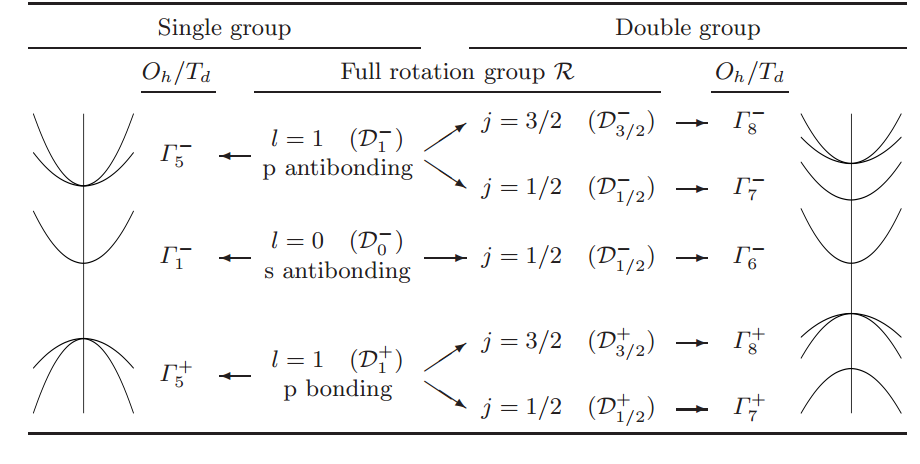
\includegraphics[width=1.0\textwidth, height=230px]{./Figures/hinh3.png}
\end{tabular}
\label{table:Symmetry}
\end{table}
\section{Mô hình Kane Mở rộng}
Khi thực hành trong tính toán ta bỏ đi số hạng thứ 2 trong phương trình trên (4.1) xem [23,20], trong mô hình $14\times14$ ta chọn 6 bonding vùng hóa trị(p) và 2 antibonding lớp ($s^*$), 6 antibonding lớp($p^*$) vùng dẫn tương tự ta chọn hàm sóng cơ sở trong hệ tọa độ hình cầu [23,9] $\vert jm\rangle $ theo trục lượng tử hóa [001]:\\
\emph{Đối với vùng} $\Gamma_{8c}$:
\[
u_1 = \left | \frac{3}{2},+\frac{3}{2}\right\rangle_{c^{'}}=\frac{-1}{\sqrt{2}}\left(
\begin{array}{cc}
X^{'} + iY^{'}\\
0
\end{array}
\right)
\qquad
u_2 = \left | \frac{3}{2},+\frac{1}{2}\right\rangle_{c^{'}}=\frac{-1}{\sqrt{6}}\left(
\begin{array}{cc}
-2Z^{'}\\
X^{'} + iY^{'}
\end{array}
\right)
\]
\[
u_3 = \left | \frac{3}{2},-\frac{1}{2}\right\rangle_{c^{'}}=\frac{1}{\sqrt{6}}\left(
\begin{array}{cc}
X^{'} - iY^{'}\\
2Z^{'}
\end{array}
\right)
\qquad
u_4 = \left | \frac{3}{2},-\frac{3}{2}\right\rangle_{c^{'}}=\frac{1}{\sqrt{2}}\left(
\begin{array}{cc}
0 \\
X^{'} - iY^{'}
\end{array}
\right)
\]
\emph{Đối với vùng} $\Gamma_{7c}$:
\[
u_5 = \left | \frac{1}{2},+\frac{1}{2}\right\rangle_{c^{'}}=\frac{-1}{\sqrt{3}}\left(
\begin{array}{cc}
Z^{'}\\
X^{'} + iY^{'}
\end{array}
\right)
\qquad
u_6= \left | \frac{1}{2},+\frac{-1}{2}\right\rangle_{c^{'}}=\frac{-1}{\sqrt{3}}\left(
\begin{array}{cc}
X^{'} - iY^{'}\\
-Z^{'}
\end{array}
\right)
\]
\emph{Đối vói vùng} $\Gamma_{6c}$:
\[
u_7 = \left | \frac{1}{2},+\frac{1}{2}\right\rangle_{c}=\left(
\begin{array}{cc}
S\\
0\end{array}
\right)
\qquad
u_8= \left | \frac{1}{2},+\frac{-1}{2}\right\rangle_{c}=\left(
\begin{array}{cc}
0\\
S
\end{array}
\right)
\]
\emph{Đối với vùng} $\Gamma_{8v}$:
\[
u_9 = \left | \frac{3}{2},+\frac{3}{2}\right\rangle_{v}=\frac{-1}{\sqrt{2}}\left(
\begin{array}{cc}
X + iY\\
0
\end{array}
\right)
\qquad
u_{10}= \left | \frac{3}{2},+\frac{1}{2}\right\rangle_{v}=\frac{-1}{\sqrt{6}}\left(
\begin{array}{cc}
-2Z\\
X + iY
\end{array}
\right)
\]
\[
u_{11} = \left | \frac{3}{2},-\frac{1}{2}\right\rangle_{v}=\frac{1}{\sqrt{6}}\left(
\begin{array}{cc}
X - iY\\
2Z
\end{array}
\right)
\qquad
u_{12} = \left | \frac{3}{2},-\frac{3}{2}\right\rangle_{v}=\frac{1}{\sqrt{2}}\left(
\begin{array}{cc}
0 \\
X - iY
\end{array}
\right)
\]
\emph{ Đối vói vùng} $\Gamma_{7v}$:
\[
u_{13} = \left | \frac{1}{2},+\frac{1}{2}\right\rangle_{v}=\frac{-1}{\sqrt{3}}\left(
\begin{array}{cc}
Z\\
X^ + iY
\end{array}
\right)
\qquad
u_{14}= \left | \frac{1}{2},+\frac{-1}{2}\right\rangle_{v}=\frac{-1}{\sqrt{3}}\left(
\begin{array}{cc}
X - iY\\
-Z
\end{array}
\right)
\]
và ta định nghĩa các ma trận mômentum và tương tác spin-orbit bởi các thông số sau [24,20,22]
\begin{align}
&\frac{\hbar}{m_0}\langle S|p_x|X\rangle = \frac{\hbar}{m_0}\langle S|p|_y|Y\rangle = \frac{\hbar}{m_0}\langle S|p_z|Z\rangle = P \notag \\
&\frac{\hbar}{m_0}\langle S|p_x|X^{'}\rangle = \frac{\hbar}{m_0}\langle S|p_y|Y^{'}\rangle = \frac{\hbar}{m_0}\langle S|p_z|Z^{'}\rangle = iP^{'} \notag\\
&\frac{\hbar}{m_0}\langle X|p_x|Z^{'}\rangle = \frac{\hbar}{m_0}\langle Y|p_y|X^{'}\rangle = \frac{\hbar}{m_0}\langle Z|p_x|Y^{'}\rangle = Q \notag\\
&\frac{-3i\hbar}{4m_0} \langle X|\left(\boldsymbol{\nabla}V_0\times p \right)_{y}|Z\rangle = \frac{-3i\hbar}{4m_0^2c^2}\langle Y|\left(\boldsymbol{\nabla}V_0\times p\right)_z|X\rangle = \frac{-3i\hbar}{4m_0^2c^2}\langle Z|\left(\boldsymbol{\nabla}V_0\times p\right)_x|Y\rangle =\Delta_0 \notag\\
&\frac{-3i\hbar}{4m_0} \langle X^{'}|\left(\boldsymbol{\nabla}V_0\times p \right)_{y}|Z^{'}\rangle = \frac{-3i\hbar}{4m_0^2c^2}\langle Y^{'}|\left(\boldsymbol{\nabla}V_0\times p\right)_z|X^{'}\rangle = \frac{-3i\hbar}{4m_0^2c^2}\langle Z^{'}|\left(\boldsymbol{\nabla}V_0\times p\right)_x|Y^{'}\rangle =\Delta_0^{'} \notag\\
&\frac{-3i\hbar}{4m_0} \langle X|\left(\boldsymbol{\nabla}V_0\times p \right)_{y}|Z^{'}\rangle = \frac{-3i\hbar}{4m_0^2c^2}\langle Y|\left(\boldsymbol{\nabla}V_0\times p\right)_z|X^{'}\rangle = \frac{-3i\hbar}{4m_0^2c^2}\langle Z|\left(\boldsymbol{\nabla}V_0\times p\right)_x|Y^{'}\rangle =i\Delta_0^{-} \notag \\
-&\frac{1}{2\sqrt{3}}\frac{\hbar^2}{m_0^2c^2}\langle X|\frac{\partial V_0}{\partial y}|Z\rangle = -\frac{1}{2\sqrt{3}}\frac{\hbar^2}{m_0^2c^2}\langle Y|\frac{\partial V_0}{\partial z}|X\rangle = -\frac{1}{2\sqrt{3}}\frac{\hbar^2}{m_0^2c^2}\langle Z|\frac{\partial V_0}{\partial x}|Y\rangle = C_k
\end{align}

\begin{figure}[hc]
\centering
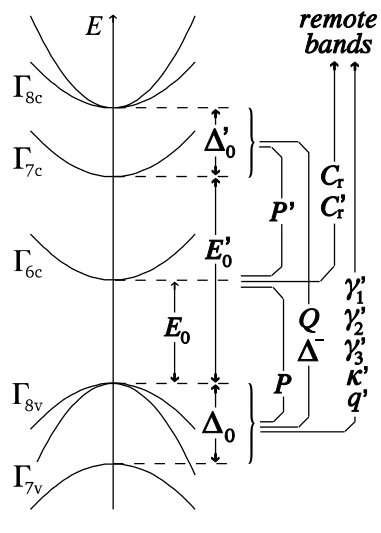
\includegraphics[width=0.50\textwidth]{./Figures/band.png}
%\rule{35em}{0.5pt}
\caption[Giản đồ cấu trúc vùng năng lượng 14 band mô hình Kane]{Giản đồ cấu trúc vùng năng lượng 14 band mô hình Kane với các tham số $P,P^{'},Q,\Delta_0,\Delta_0^{-},C_k $ được định nghĩa ở trên Ref[22].}
\end{figure}


\section{Phân tích các thành phần Hamiltonian}
\begin{enumerate}
\item[1/]\textbf{Số hạng tương tác kp:} $\langle u_i|\mathcal{H}_{kp}|u_j\rangle$
ký hiệu các trạng spin up$| \uparrow\rangle$, và spin down$|\downarrow\rangle$ và có tính chất sau:
\begin{align}
\langle \uparrow |\uparrow\rangle = \langle\downarrow |\downarrow\rangle =1,\langle \uparrow |\downarrow\rangle = \langle\downarrow |\uparrow\rangle =0
\end{align}
\begin{align*}
\mathcal{H}_{17}&=\frac{\hbar}{m_0}\Bigl\langle u_1\Bigl\vert \mathbf{kp}\Bigr\vert u_7\Bigr\rangle = \frac{-\hbar}{\sqrt{2}m_0}\Bigl\langle X^{'} -iY^{'}\Bigr\vert\mathbf{kp}\Bigl\vert S\Bigr\rangle \Bigl\langle\Bigl\uparrow \Bigl\vert \Bigr\uparrow\Bigr\rangle 
= \frac{-\hbar}{\sqrt{2}m_0}\Bigl[\Bigl\langle X^{'}\Bigl\vert \mathbf{kp}\Bigr\vert S\Bigr\rangle -i\Bigl\langle Y^{'}\Bigl\vert \mathbf{kp}\Bigr\vert S\Bigr\rangle\Bigr] \\
&=\frac{-\hbar}{\sqrt{2}m_0}\Bigl[\Bigl\langle X^{'}\Bigl\vert \mathbf{k_x p_x}\Bigr\vert S\Bigr\rangle -i\Bigl\langle Y^{'}\Bigl\vert \mathbf{k_x p_x}\Bigr\vert S\Bigr\rangle\Bigr]=\frac{1}{2}iP^{'}\left(k_x -ik_y\right)=\frac{1}{\sqrt{2}}iP^{'}k_{\_}
\end{align*}
\begin{align*}
\mathcal{H}_{71}&=\frac{\hbar}{m_0}\Bigl\langle u_7\Bigl\vert \mathbf{kp}\Bigr\vert u_1\Bigr\rangle  =
\frac{-\hbar}{\sqrt{2}m_0}\Bigl\langle S\Bigl\vert\mathbf{kp}\Bigr\vert X^{'} +iY^{'}\Bigr\rangle \Bigl\langle \Bigl\uparrow \Bigl\vert  \Bigr\uparrow
\Bigr\rangle =
\frac{-\hbar}{\sqrt{2}m_0}\Bigl[\Bigl\langle S\Bigl\vert \mathbf{kp}\Bigl\vert X^{'}\Bigr\rangle + i\Bigl\langle S\Bigl\vert \mathbf{kp}\Bigr\vert Y^{'}\Bigr\rangle\Bigr]\\
&=\frac{-\hbar}{\sqrt{2}m_0}\Bigl[\Bigl\langle S\Bigl\vert \mathbf{k_x p_x}\Bigr\vert X^{'}\Bigr \rangle +i\Bigl\langle S\Bigl\vert \mathbf{k_x p_x}\Bigr\vert Y^{'} \Bigr\rangle\Bigr]
=\frac{-1}{2}iP^{'}\left(k_x +ik_y\right)=\frac{-1}{\sqrt{2}}iP^{'}k_{+}
\end{align*}
để ý $\mathcal{H}_{71} = \left(\mathcal{H}_{17}\right)^*$, các số hạng kp còn lại ta tính tương tự.
\item[2/]\textbf{Số hạng tương tác SO}:\\
ta chú ý $\sigma_x|\uparrow\rangle = |\downarrow\rangle,\sigma_x|\downarrow\rangle = |\uparrow\rangle,\sigma_y|\uparrow\rangle = -i|\uparrow\rangle,\sigma_y|\downarrow\rangle = i|\downarrow\rangle,\sigma_z|\uparrow\rangle = |\uparrow\rangle,\sigma_z|\downarrow \rangle = |\downarrow\rangle$
\begin{align*}
\mathcal{H}_{11}&=\Bigl\langle u_1\Bigl\vert \boldsymbol{\sigma}\left(\nabla\times p\right)\Bigr\vert u_1\Bigr\rangle =
 \frac{1}{2}\left\langle \left(X^{'}-iY^{'}\right)\Bigl\uparrow \Bigl\vert \boldsymbol{\sigma}\left(\nabla V\times p\right)\Bigr\vert \Bigr\uparrow \left(X^{'}+iY^{'}\right)\right\rangle \\
 &=\frac{1}{2}\left\langle \left(X^{'}-iY^{'}\right) \Bigl\vert \left(\nabla V\times p\right)\Bigr\vert \left(X^{'}+iY^{'}\right)\right\rangle \left\langle \Bigl\uparrow \Bigl\vert \boldsymbol{\sigma}\Bigr\vert \Bigr\uparrow\right\rangle
\end{align*}
mà $\langle \uparrow|\boldsymbol{\sigma}|\uparrow\rangle = \langle \uparrow|\uparrow\rangle=1$ ứng với trường hợp $\sigma=\sigma_z$ còn các trường hợp khác bằng không nên:
\begin{align*}
\Longrightarrow
\mathcal{H}_{11}&= \frac{1}{2}\left\langle \left(X^{'}-iY^{'}\right) \left |\left(\nabla V\times p\right)_z\right | \left(X^{'}+iY^{'}\right)\right\rangle \\
&= \frac{1}{2}\left\langle X^{'} \left |\left(\nabla V\times p\right)_z\right | iY^{'}\right\rangle -i \frac{1}{2}\left\langle Y^{'} \left |\left(\nabla V\times p\right)_z\right |X^{'}\right\rangle = i\left\langle X^{'} \left |\left(\nabla V\times p\right)_z\right | Y^{'}\right\rangle
\end{align*}
mặc khác khi ta tính $\mathcal{H}_{11}$ ta chưa thêm số hạng $\frac{\hbar}{4n_0^2c^2}$ do đó ta viêt lại số hạng $\mathcal{H}_{11}$ như sau:
\begin{equation}
\mathcal{H}_{11}=\frac{i\hbar}{4m_0^2c^2}\left(\langle X^{'}\Bigl\vert \left(\nabla V\times p\right)_z\Bigr\vert Y^{'}\right\rangle = \frac{\Delta^{'}}{3}
\end{equation}
Tương tự ta tính lại các số hạng SO như ở trên, cuối cùng ta thây các kết quả ở số hạng kp ,số hạng SO đồng thời số hạng đầu tiên ở phương trình (4.3) chú ý $\delta_{nn}=1,\delta_{nm}=0$ vậy ta có ma trận Hamiltonian như sau:
\end{enumerate}
\begin{equation}
\mathcal{H}_{14\times 14} =
\begin{pmatrix}
\mathcal{H}_{8c8c} & \mathcal{H}_{8c7c} & \mathcal{H}_{8c6c} & \mathcal{H}_{8c8v} & \mathcal{H}_{8c7v}\\
\mathcal{H}_{7c8c} & \mathcal{H}_{7c7v} & \mathcal{H}_{7c6c} & \mathcal{H}_{7c8v} & \mathcal{H}_{7c7v}\\
\mathcal{H}_{6c8c} & \mathcal{H}_{6c7c} & \mathcal{H}_{6c6c} & \mathcal{H}_{6c8v} & \mathcal{H}_{6c7v}\\
\mathcal{H}_{8v8c} & \mathcal{H}_{8v7c} & \mathcal{H}_{8v6c} & \mathcal{H}_{8v8v} & \mathcal{H}_{8v7v}\\
\mathcal{H}_{7v8c} & \mathcal{H}_{7v7c} & \mathcal{H}_{7v6c} & \mathcal{H}_{7v8v} & \mathcal{H}_{7v7v}
\end{pmatrix}
\end{equation}
ở đây:
\begin{align*}
\mathcal{H}_{8c8c}&=\begin{pmatrix}
E_g^{'}+\Delta^{'} & 0 & 0 & 0 \\
0 & E_g^{'}+\Delta^{'} & 0  & 0 \\
0 &0 &E_g^{'}+\Delta^{'} & 0 \\
& 0 & 0 & 0 &E_g^{'}+\Delta^{'} 
\end{pmatrix}\qquad
\mathcal{H}_{8c7c}=\begin{pmatrix}
0 & 0 \\
0 & 0 \\
0 & 0 \\
0 & 0 
\end{pmatrix}\\
\mathcal{H}_{8c6c}&=\begin{pmatrix}
\frac{1}{\sqrt{2}}iP^{'}k_\_  &0\\
-\sqrt{\frac{2}{3}}iP^{'}k_z & \sqrt{\frac{1}{6}}iP^{'}k_\_ \\
-\sqrt{\frac{1}{6}}iP^{'}k_+ & -\sqrt{\frac{2}{3}}iP^{'}k_z \\
0 & -\frac{1}{\sqrt{2}}iP^{'}k_+ 
\end{pmatrix}\qquad
\mathcal{H}_{8c8v}=\begin{pmatrix}
\frac{i\overline{\Delta}}{3} &\sqrt{\frac{1}{3}}iQk_+ & \sqrt{\frac{1}{3}}iQk_z & 0\\
-\sqrt{\frac{1}{3}}iQk_\_ &\frac{i\overline{\Delta}}{3} &0 & \sqrt{\frac{1}{3}}iQk_z\\
-\sqrt{\frac{1}{3}}iQk_z &0 &\frac{i\overline{\Delta}}{3} &-\sqrt{\frac{1}{3}}iQk_+\\
 0  &-\sqrt{\frac{1}{3}}iQk_z & \sqrt{\frac{1}{3}}iQk_\_ &\frac{i\overline{\Delta}}{3}
\end{pmatrix}\\
\mathcal{H}_{8c7v}&=\begin{pmatrix}
-\sqrt{\frac{1}{6}}iQk_+ &-\sqrt{\frac{2}{3}}iQk_z \\
0 &\sqrt{\frac{1}{2}}iQk_+ \\
-\sqrt{\frac{1}{6}}iQk_\_ &0\\
-\sqrt{\frac{2}{3}}iQk_z &-\sqrt{\frac{1}{6}}iQk_+
\end{pmatrix}\qquad
\mathcal{H}_{7c7c}=\begin{pmatrix}
 E_g^{'} &0\\
 0 &E_g^{'}
\end{pmatrix}\qquad
\mathcal{H}_{7c6c}=\begin{pmatrix}
 \sqrt{\frac{1}{3}}iP^{'}k_z & \sqrt{\frac{1}{3}}iP^{'}k_\_ \\
 \sqrt{\frac{1}{3}}iP^{'}k_+ & -\sqrt{\frac{1}{3}}iP^{'}k_z
\end{pmatrix}\\
\mathcal{H}_{7c8v}&=\begin{pmatrix}
\sqrt{\frac{1}{6}} iQk_\_ &0 &\sqrt{\frac{1}{2}}iQk_+ &\sqrt{\frac{2}{3}} iQk_z\\
\sqrt{\frac{2}{3}} iQk_z &\sqrt{\frac{1}{2}} iQk_\_ &0 &-\sqrt{\frac{1}{6}} iQk_+
\end{pmatrix}\qquad
\mathcal{H}_{7c7v}=\begin{pmatrix}
-\frac{2}{3}i\overline{\Delta} &0\\
0 &-\frac{2}{3}i\overline{\Delta}
\end{pmatrix}\\
\mathcal{H}_{6c6c}&=\begin{pmatrix}
E_g +\frac{\hbar^2k^2}{2m_0} & 0\\
0 &E_g +\frac{\hbar^2k^2}{2m_0}
\end{pmatrix}\qquad
\mathcal{H}_{6c8v}=\begin{pmatrix}
-\sqrt{\frac{1}{2}}Pk_+ &\sqrt{\frac{2}{3}}Pk_z &\sqrt{\frac{1}{6}}Pk_\_ &0 \\
0 &-\sqrt{\frac{1}{6}}Pk_+ &\sqrt{\frac{2}{3}}Pk_z &\sqrt{\frac{1}{2}}Pk_\_
\end{pmatrix}\\
\mathcal{H}_{6c7v}&=\begin{pmatrix}
-\sqrt{\frac{1}{3}}pk_z &-\sqrt{\frac{1}{3}}Pk_\_\\
-\sqrt{\frac{1}{3}}pk_+ &\sqrt{\frac{1}{3}}Pk_z
\end{pmatrix}\qquad
\mathcal{H}_{8v8v}=\begin{pmatrix}
\frac{\hbar^2k^2}{2m_0} & -\frac{1}{2}C_{k}k_+ & C_k k_z &-\frac{\sqrt{3}}{2}C_k k_\_ \\
-\frac{1}{2}C_{k}k_\_ &\frac{\hbar^2k^2}{2m_0} &\frac{\sqrt{3}}{2}c_k k_\_ &-C_k k_z \\
C_kk_z &\frac{\sqrt{3}}{2}C_kk_\_  &\frac{\hbar^2k^2}{2m_0} &-\frac{1}{2}C_{k}k_+\\
-\frac{\sqrt{3}}{2}C_kk_+ &-C_kk_z &-\frac{1}{2}C_{k}k_\_ &\frac{\hbar^2k^2}{2m_0}
\end{pmatrix}\\
\mathcal{H}_{8v7v}&=\begin{pmatrix}
\frac{1}{2\sqrt{2}}C_{k}k_\_ &\sqrt{\frac{1}{2}}C_{k}k_z \\
0 & -\frac{3}{2\sqrt{6}}C_{k}k_+ \\
\frac{3}{2\sqrt{6}}C_{k}k_\_ &0 \\
\sqrt{\frac{1}{2}}C_{k }k_z &-\frac{1}{2\sqrt{2}}C_k k_\_
\end{pmatrix}\qquad
\mathcal{H}_{7v7v}=\begin{pmatrix}
\frac{\hbar^2k^2}{2m_0}-\Delta &0\\
0 &\frac{\hbar^2k^2}{2m_0}-\Delta
\end{pmatrix}
\end{align*}
với $k^2=k_x^2 +k_y^2+k_z^2$ và $k_{\pm}=k_x \pm ik_y$.Còn các tham số $E_g,E_g^{'},\Delta,\Delta^{'},\Delta^{-},P,P^{'},Q,C_k$ được định nghĩa ở biểu thức (4.5) giá trị thực nghiệm của nó được cho ở bản 4.3, như đã nói ở trên để có độ chính xác cao ta cần thây dổi các Hamiltonian ở vùng hóa trị bằng các Hamiltonian tính được nhờ phương pháp nhiễu loạn L$\ddot{o}$wdin. Ta sẽ thảo luận ở mục tiếp theo sử dụng kết quả mục 4.4 ta có thể viết lại các thành phần ma trận Hamiltonian:
\begin{align*}
\mathcal{H}_{6c6c}&=\begin{pmatrix}
E_g +\frac{\hbar^2k^2}{2m^{'}} & 0\\
0 &E_g +\frac{\hbar^2k^2}{2m^{'}}
\end{pmatrix}
\qquad
\mathcal{H}_{7v7v}=\begin{pmatrix}
-\frac{\hbar^2k^2}{2m_0}\gamma_1^{'} -\Delta & 0\\
0 &-\frac{\hbar^2k^2}{2m_0}\gamma_1^{'} -\Delta
\end{pmatrix}
\\
\mathcal{H}_{8v7v}&=\begin{pmatrix}
-\frac{\sqrt{6}\hbar^2}{2m_0}\gamma_3^{'}k_\_k_z +\frac{1}{2\sqrt{2}}C_kk_\_& -\frac{\sqrt{6}\hbar^2}{2m_0}\left(\gamma_2^{'}(k_x^2 - k_y^2) - 2i\gamma_3^{'}k_xk_y\right) +\sqrt{\frac{1}{2}}C_kk_z\\
-\frac{\sqrt{2}\hbar^2}{2m_0}\gamma_3^{'}(k_x^2 +k_y^2 - 2k_z^2) &\frac{3\sqrt{2}\hbar^2}{2m_0}\gamma_3^{'}k_\_k_z -\frac{\sqrt{6}}{4}C_kk_+ \\
\frac{3\sqrt{2}\hbar^2}{2m_0}\gamma_3^{'}k_+k_z +\frac{\sqrt{6}}{4}C_kk_\_ &\frac{\sqrt{2}\hbar^2}{2m_0}\gamma_3^{'}(k_x^2 +k_y^2 - 2k_z^2)\\
\frac{\sqrt{6}\hbar^2}{2m_0}\left(\gamma_2^{'}(k_x^2 - k_y^2) + 2i\gamma_3^{'}k_xk_y\right) +\sqrt{\frac{1}{2}}C_kk_z &\frac{\sqrt{6}\hbar^2}{2m_0}\gamma_3^{'}k_\_k_z - \frac{1}{2\sqrt{2}}C_kk_\_
\end{pmatrix}\\
 \mathcal{H}_{8v8v} &=\left(
 \begin{array}{c|c|c|c}
\begin{array}{c}
-\frac{\hbar^2(\gamma_1^{'} +\gamma_2^{'})(ik_x^2 +k_y^2)}{2m_0}\\
-\frac{\hbar^2(\gamma_1^{'}-2\gamma_2^{'})k_z^2}{2m_0} 
\end{array}
&\begin{array}{c}
 \frac{2\sqrt{3}\hbar^2\gamma_3^{'}k_zk_\_}{2m_0} \\
-\frac{1}{2}C_kk_+
\end{array}
&\begin{array}{c}
\frac{\sqrt{3}\hbar^2\gamma_2^{'}(k_x^2 -k_y^2)}{2m_0} \\
-\frac{2\sqrt{3}i\hbar^2\gamma_3^{'}k_xk_y}{2m_0}\\
+C_kk_z
\end{array}
&\begin{array}{c}
\frac{\sqrt{3}}{2}C_kk_\_
\end{array}
\\ \hline
\begin{array}{c}
\frac{2\sqrt{3}\hbar^2\gamma_3^{'}k_zk_+}{2m_0} \\
-\frac{1}{2}C_kk_\_
\end{array}
&\begin{array}{c}
 -\frac{\hbar^2(\gamma_1^{'} -\gamma_2^{'})(ik_x^2 +k_y^2)}{2m_0}\\
-\frac{\hbar^2(\gamma_1^{'}+2\gamma_2^{'})k_z^2}{2m_0} 
\end{array}
&\begin{array}{c}
\frac{\sqrt{3}}{2}C_kk_+
\end{array}
&\begin{array}{c}
\frac{\sqrt{3}\hbar^2\gamma_2^{'}(k_x^2 -k_y^2)}{2m_0} \\
+\frac{2\sqrt{3}i\hbar^2\gamma_3^{'}k_xk_y}{2m_0}\\
-C_kk_z
\end{array}
\\ \hline
\begin{array}{c}
\frac{\sqrt{3}\hbar^2\gamma_2^{'}(k_x^2 -k_y^2)}{2m_0} \\
+\frac{2\sqrt{3}i\hbar^2\gamma_3^{'}k_xk_y}{2m_0}\\
+C_kk_z
\end{array}
&\begin{array}{c}
\frac{\sqrt{3}}{2}C_kk_\_
\end{array}
&\begin{array}{c}
-\frac{\hbar^2(\gamma_1^{'}-\gamma_2^{'})(ik_x^2 +k_y^2)}{2m_0}\\
-\frac{\hbar^2(\gamma_1^{'}+2\gamma_2^{'})k_z^2}{2m_0} 
\end{array}
&\begin{array}{c}
- \frac{2\sqrt{3}\hbar^2\gamma_3^{'}k_zk_\_}{2m_0} \\
-\frac{1}{2}C_kk_+
\end{array}
\\ \hline
\begin{array}{c}
\frac{\sqrt{3}}{2}C_kk_+
\end{array}
&\begin{array}{c}
\frac{\sqrt{3}\hbar^2\gamma_2^{'}(k_x^2 -k_y^2)}{2m_0} \\
+\frac{2\sqrt{3}i\hbar^2\gamma_3^{'}k_xk_y}{2m_0}\\
-C_kk_z
\end{array}
&\begin{array}{c}
- \frac{2\sqrt{3}\hbar^2\gamma_3^{'}k_zk_+}{2m_0} \\
-\frac{1}{2}C_kk_\_
\end{array}
&\begin{array}{c}
-\frac{\hbar^2(\gamma_1^{'}-\gamma_2^{'})(ik_x^2 +k_y^2)}{2m_0}\\
-\frac{\hbar^2(\gamma_1^{'}+2\gamma_2^{'})k_z^2}{2m_0} 
\end{array}
\end{array}\right)
\end{align*}


\section{Biến đổi tọa độ}
Ở trên chúng ta đang xét tinh thể theo chiều [001] ($\mathbf{k}=k\mathbf{\hat{z}}$) trong tọa độ ĐềCat, trong trường hợp tổng quát véctơ sóng $\mathbf{k}$ không hướng theo trục nào cả thì ta cần biến đổi chúng bởi phép quay Euler $\mathcal{R}$(xem mục 2.4)
\begin{align*}
\mathcal{R}&= \mathcal{R}_z(\alpha)\mathcal{R}_y(\beta)\mathcal{R}_{\mathit{x}}(\gamma)
=\mathcal{R}_z(\alpha)\mathcal{R}_y(\beta)\mathcal{R}_z(\gamma)\\
&=\begin{pmatrix}
\cos\alpha &-sin\alpha & 0\\
\sin\alpha &\cos\alpha &0\\
0 &0 &1
\end{pmatrix}
\begin{pmatrix}
\cos\beta &0 &sin\beta\\
0 &1 & 0\\
-\sin\beta &0 &\cos\beta
\end{pmatrix}
\begin{pmatrix}
1 &0 &0 \\
0 &\cos\gamma &-\sin\gamma\\
0 &\sin\gamma &\cos\gamma
\end{pmatrix}\\
&=\begin{pmatrix}
\cos\alpha &-sin\alpha & 0\\
\sin\alpha &\cos\alpha &0\\
0 &0 &1
\end{pmatrix}
\begin{pmatrix}
\cos\beta &0 &sin\beta\\
0 &1 & 0\\
-\sin\beta &0 &\cos\beta
\end{pmatrix}
\begin{pmatrix}
\cos\gamma &-\sin\gamma &0\\
\sin\gamma &\cos\gamma &0\\
0 &0 &1
\end{pmatrix}
\end{align*} 
do đó véctơ xung lượng $\mathbf{k}^{'}$có mối liên hệ với $\mathbf{k}$ như sau:
\begin{equation}
\begin{pmatrix}
k_{\mathit{x}}^{'} \\k_y^{'} \\k_z^{'}\end{pmatrix}
 = \mathcal{R}\begin{pmatrix}
k_{\mathit{x}} \\k_y \\k_z
\end{pmatrix}
\end{equation}
toán tử của phép quay ứng với $j=1/2,j=3/2$ có dạng sau đây:
\begin{equation}
\mathcal{D}_{1/2}=\begin{pmatrix}
exp(-i\frac{\alpha}{2}) &0\\
0 &exp(i\frac{\alpha}{2}
\end{pmatrix}
\begin{pmatrix}
\cos(\frac{\beta}{2}) &-\sin(\frac{\beta}{2})\\
\sin(\frac{\beta}{2}) &\cos(\frac{\beta}{2})\\
\end{pmatrix}
\begin{pmatrix}
exp(-i\frac{\gamma}{2}) &0\\
0 &exp(i\frac{\gamma}{2})
\end{pmatrix}
\end{equation}
và
\begin{align}
\mathcal{D}_{3/2}=&\begin{pmatrix}
exp(-i\frac{3}{2}\alpha) &0 &0 &0\\
0 &exp(-i\frac{3}{2}\alpha) &0 &0 \\
0& 0& exp(i\frac{3}{2}\alpha) &0 \\
0 &0 &0 &exp(i\frac{3}{2}\alpha)
\end{pmatrix}\notag\\
\times&\begin{pmatrix}
\cos^{3}(\frac{\beta}{2}) &-\sqrt{3}\cos^{2}(\frac{\beta}{2})\sin(\frac{\beta}{2}) &\sqrt{3}\cos^{}(\frac{\beta}{2})\sin(\frac{\beta}{2}) &-\sin^{3}(\frac{\beta}{2})\\
\sqrt{3}\cos^{2}(\frac{\beta}{2})\sin(\frac{\beta}{2}) &\cos^{3}(\frac{\beta}{2})-2\cos(\frac{\beta}{2})\sin^{2}(\frac{\beta}{2}) &-2\cos^{2}(\frac{\beta}{2})\sin(\frac{\beta}{2}) +\sin^{3}(\frac{\beta}{2}) &\sqrt{3}\cos^{2}(\frac{\beta}{2})\sin(\frac{\beta}{2})\\
\sqrt{3}\cos(\frac{\beta}{2})\sin^{2}(\frac{\beta}{2}) &2\cos^{2}(\frac{\beta}{2})\sin(\frac{\beta}{2})-\sin^{3}(\frac{\beta}{2}) &\cos^{3}(\frac{\beta}{2})-2\cos(\frac{\beta}{2})\sin^{2}(\frac{\beta}{2}) &-\sqrt{3}\cos^{2}(\frac{\beta}{2})\sin(\frac{\beta}{2})\\
\sin^{3}(\frac{\beta}{2}) &\sqrt{3}\cos(\frac{\beta}{2})\sin^{2}(\frac{\beta}{2}) &\sqrt{3}\cos^{2}(\frac{\beta}{2})\sin(\frac{\beta}{2})  &\cos^{3}(\frac{\beta}{2})
\end{pmatrix}\notag\\
\times&\begin{pmatrix}
exp(-i\frac{3}{2}\gamma) &0 &0 &0\\
0 &exp(-i\frac{3}{2}\gamma) &0 &0 \\
0& 0&exp(i\frac{3}{2}\gamma) &0 \\
0 &0 &0 &exp(i\frac{3}{2}\gamma)
\end{pmatrix}
\end{align}
còn Hamiltonian trong hệ tọa độ mới có dạng sau:
\begin{align}
&\mathcal{H}_{14\times14}^{'}=\begin{pmatrix}
\mathcal{H}_{8c8c}^{'} & \mathcal{H}_{8c7c}^{'} & \mathcal{H}_{8c6c}^{'} & \mathcal{H}_{8c8v}^{'} & \mathcal{H}_{8c7v}^{'}\\
\mathcal{H}_{7c8c}^{'} & \mathcal{H}_{7c7v}^{'} & \mathcal{H}_{7c6c}^{'} & \mathcal{H}_{7c8v}^{'} & \mathcal{H}_{7c7v}^{'}\\
\mathcal{H}_{6c8c}^{'} & \mathcal{H}_{6c7c}^{'} & \mathcal{H}_{6c6c}^{'} & \mathcal{H}_{6c8v}^{'} & \mathcal{H}_{6c7v}^{'}\\
\mathcal{H}_{8v8c}^{'} & \mathcal{H}_{8v7c}^{'} & \mathcal{H}_{8v6c}^{'} & \mathcal{H}_{8v8v}^{'} & \mathcal{H}_{8v7v}^{'}\\
\mathcal{H}_{7v8c}^{'} & \mathcal{H}_{7v7c}^{'} & \mathcal{H}_{7v6c}^{'} & \mathcal{H}_{7v8v}^{'} & \mathcal{H}_{7v7v}^{'}
\end{pmatrix}\notag\\
&=\begin{pmatrix}
\mathcal{D}_{3/2}^{\dagger} \mathcal{H}_{8c8c}\mathcal{D}_{3/2} & \mathcal{D}_{3/2}^{\dagger}\mathcal{H}_{8c7c}\mathcal{D}_{1/2} & \mathcal{D}_{3/2}^{\dagger}\mathcal{H}_{8c6c}\mathcal{D}_{1/2} & \mathcal{D}_{3/2}^{\dagger}\mathcal{H}_{8c8v}\mathcal{D}_{3/2}& \mathcal{D}_{3/2}^{\dagger}\mathcal{H}_{8c7v}\mathcal{D}_{1/2}\\
\mathcal{D}_{1/2}^{\dagger}\mathcal{H}_{7c8c}\mathcal{D}_{3/2} & \mathcal{D}_{1/2}^{\dagger}\mathcal{H}_{7c7v}\mathcal{D}_{1/2} & \mathcal{D}_{1/2}^{\dagger}\mathcal{H}_{7c6c}\mathcal{D}_{1/2} & \mathcal{D}_{1/2}^{\dagger}\mathcal{H}_{7c8v}\mathcal{D}_{3/2} &
\mathcal{D}_{1/2}^{\dagger} \mathcal{H}_{7c7v}\mathcal{D}_{1/2}\\
\mathcal{D}_{1/2}^{\dagger}\mathcal{H}_{6c8c}\mathcal{D}_{3/2} & \mathcal{D}_{1/2}^{\dagger}\mathcal{H}_{6c7c}\mathcal{D}_{1/2} &
\mathcal{D}_{1/2}^{\dagger} \mathcal{H}_{6c6c}\mathcal{D}_{1/2} & \mathcal{D}_{1/2}^{\dagger}\mathcal{H}_{6c8v}\mathcal{D}_{3/2} & \mathcal{D}_{1/2}^{\dagger}\mathcal{H}_{6c7v}\mathcal{D}_{1/2}\\
\mathcal{D}_{3/2}^{\dagger}\mathcal{H}_{8v8c}\mathcal{D}_{3/2} & \mathcal{D}_{3/2}^{\dagger}\mathcal{H}_{8v7c}\mathcal{D}_{1/2} & \mathcal{D}_{3/2}^{\dagger}\mathcal{H}_{8v6c}\mathcal{D}_{1/2} & \mathcal{D}_{3/2}^{\dagger}\mathcal{H}_{8v8v}\mathcal{D}_{3/2} &
\mathcal{D}_{3/2}^{\dagger} \mathcal{H}_{8v7v}\mathcal{D}_{1/2}\\
\mathcal{D}_{1/2}^{\dagger}\mathcal{H}_{7v8c}\mathcal{D}_{3/2} & \mathcal{D}_{1/2}^{\dagger}\mathcal{H}_{7v7c}\mathcal{D}_{1/2} & \mathcal{D}_{1/2}^{\dagger}\mathcal{H}_{7v6c}\mathcal{D}_{1/2} & \mathcal{D}_{1/2}^{\dagger}\mathcal{H}_{7v8v}\mathcal{D}_{3/2} & \mathcal{D}_{1/2}^{\dagger}\mathcal{H}_{7v7v}\mathcal{D}_{1/2}
\end{pmatrix}
\end{align}
kế đó ta cho các giá trị của phép quay Euler $\alpha=\pi/4,\beta=\pi/2,\gamma=0$, thì ta sẽ có một hệ tọa độ mới tương ứng với các trục sau $\mathit{x}||[00\overline{1}],y||[\overline{1}10],z||[110]$. Do đó lúc này các thành phần ma trận trong phương trình (4.8) có dạng sau:
\begin{align*}
\mathcal{H}_{8c8c}&=\begin{pmatrix}
E_g^{'}+\Delta^{'} & 0 & 0 & 0 \\
0 & E_g^{'}+\Delta^{'} & 0  & 0 \\
0 &0 &E_g^{'}+\Delta^{'} & 0 \\
& 0 & 0 & 0 &E_g^{'}+\Delta^{'} 
\end{pmatrix}\qquad
\mathcal{H}_{8c7c}=\begin{pmatrix}
0 & 0 \\
0 & 0 \\
0 & 0 \\
0 & 0 
\end{pmatrix}\\
\mathcal{H}_{8c6c}&=\begin{pmatrix}
\frac{1}{\sqrt{2}}iP^{'}k_\_^{'}  &0\\
-\sqrt{\frac{2}{3}}iP^{'}k_z^{'}  & \sqrt{\frac{1}{6}}iP^{'}k_\_^{'}  \\
-\sqrt{\frac{1}{6}}iP^{'}k_+^{'}  & -\sqrt{\frac{2}{3}}iP^{'}k_z^{'}  \\
0 & -\frac{1}{\sqrt{2}}iP^{'}k_+^{'}  
\end{pmatrix}\qquad
\mathcal{H}_{8c8v}=\begin{pmatrix}
\frac{i\overline{\Delta}}{3}+\frac{Qk_x^{'}}{3} &\sqrt{\frac{1}{3}}iQk_z^{'}  &\frac{Q(k_x^{'}+2ik_y^{'})}{2\sqrt{3}}  & 0\\
-\sqrt{\frac{1}{3}}Qk_z^{'}  &\frac{i\overline{\Delta}}{3} -\frac{Qk_x^{'}}{2} &0 & \frac{Q(k_x^{'}+2ik_y^{'})}{2\sqrt{3}} \\
\frac{Q(k_x^{'}-2ik_y^{'})}{2\sqrt{3}}  &0 &\frac{i\overline{\Delta}}{3}+\frac{Qk_x^{'}}{3} &-\sqrt{\frac{1}{3}}iQk_z^{'} \\
 0  &\frac{Q(k_x^{'}-2ik_y^{'})}{2\sqrt{3}}   & \sqrt{\frac{1}{3}}iQk_z^{'}  &-\frac{i\overline{\Delta}}{3}+\frac{Qk_x^{'}}{3} 
\end{pmatrix}\\
\mathcal{H}_{8c7v}&=\begin{pmatrix}
-\sqrt{\frac{1}{6}}Qk_z^{'}  &-\frac{Q(k_x^{'}+2ik_y^{'})}{\sqrt{6}} \\
 \sqrt{\frac{1}{2}}Qk_x^{'}&\sqrt{\frac{1}{2}}Qk_z^{'}  \\
 \sqrt{\frac{1}{2}}Qk_x^{'}&-\sqrt{\frac{1}{2}}Qk_z^{'}  \\
-\sqrt{\frac{2}{3}}iQk_z^{'}  &-\sqrt{\frac{1}{6}}Qk_z^{'}
\end{pmatrix}\qquad
\mathcal{H}_{7c7c}=\begin{pmatrix}
 E_g^{'} &0\\
 0 &E_g^{'}
\end{pmatrix}\qquad
\mathcal{H}_{7c6c}=\begin{pmatrix}
 \sqrt{\frac{1}{3}}iP^{'}k_z^{'}  & \sqrt{\frac{1}{3}}iP^{'}k_\_^{'}  \\
 \sqrt{\frac{1}{3}}iP^{'}k_+^{'}  & -\sqrt{\frac{1}{3}}iP^{'}k_z^{'} 
\end{pmatrix}\\
\mathcal{H}_{7c8v}&=\begin{pmatrix}
-\sqrt{\frac{1}{6}} iQk_z^{'} &\sqrt{\frac{1}{2}}iQk_x^{'} &\sqrt{\frac{1}{2}}iQk_z^{'} &\sqrt{\frac{1}{}}iQ(k_x^{'}+2ik_y^{'})\\
\sqrt{\frac{1}{}}iQ(k_x^{'}+2ik_y^{'}) &\sqrt{\frac{1}{2}}iQk_z &\sqrt{\frac{1}{2}} iQk_x^{'} &-\sqrt{\frac{1}{6}}iQk_z^{'}
\end{pmatrix}\qquad
\mathcal{H}_{7c7v}=\begin{pmatrix}
-\frac{2}{3}i\overline{\Delta} &0\\
0 &-\frac{2}{3}i\overline{\Delta}
\end{pmatrix}\\
\mathcal{H}_{6c6c}&=\begin{pmatrix}
E_g +\frac{\hbar^2k^{'2}}{2m_0} & 0\\
0 &E_g +\frac{\hbar^2k^{'2}}{2m_0}
\end{pmatrix}\qquad
\mathcal{H}_{6c8v}=\begin{pmatrix}
-\sqrt{\frac{1}{2}}Pk_+^{'}  &\sqrt{\frac{2}{3}}Pk_z^{'}  &\sqrt{\frac{1}{6}}Pk_\_^{'}  &0 \\
0 &-\sqrt{\frac{1}{6}}Pk_+^{'}  &\sqrt{\frac{2}{3}}Pk_z^{'}  &\sqrt{\frac{1}{2}}Pk_\_^{'} 
\end{pmatrix}\\
\mathcal{H}_{6c7v}&=\begin{pmatrix}
-\sqrt{\frac{1}{3}}pk_z^{'}  &-\sqrt{\frac{1}{3}}Pk_\_^{'} \\
-\sqrt{\frac{1}{3}}pk_+^{'}  &\sqrt{\frac{1}{3}}Pk_z^{'} 
\end{pmatrix}\qquad
\mathcal{H}_{7v7v}=\begin{pmatrix}
-\frac{\hbar^2k^{'2}}{2m_0}\gamma_1^{'}-\Delta &0\\
0 &-\frac{\hbar^2k^{'2}}{2m_0}\gamma_1^{'}-\Delta
\end{pmatrix}
\end{align*}
%matrix-------------------------------------> H8v7v
\begin{align*}
\mathcal{H}_{8v7v} &=\left(
 \begin{array}{c|c}
\begin{array}{c}
-\frac{\sqrt{6}\hbar^2(\gamma_3^{'}k_x^{'} -i\gamma^{'} -2k_y^{'})k_z^{'}}{2m_0} -\frac{iC_kk_z^{'}}{2\sqrt{2}}
\end{array}
&\begin{array}{c}
 -\frac{\sqrt{6}\hbar^2(2\gamma_2^{'}k_x^{'2} -4i\gamma_3^{'}k_x^{'}k_y^{'} -(\gamma_2^{'}+\gamma_3^{'})k_y^{'2}-(\gamma_2^{'}-\gamma_3^{'})k_z^{'2}}{2m_0}\\
 +\frac{C_k(2k_y -ik_x^{'2})}{ 2\sqrt{2}}
\end{array}
\\ \hline
\begin{array}{c}
-\frac{\hbar^2(2\gamma_2^{'}k_x^{'2} -(\gamma_2^{'}+\gamma_3^{'})k_z^{'2}-(\gamma_2^{'}-\gamma_3^{'})k_y^{'2}}{2\sqrt{2}m_0}+\frac{\sqrt{3}iC_kk_x^{'}}{ 2\sqrt{2}}
\end{array}
&\begin{array}{c}
-\frac{3\sqrt{2}\hbar^2(\gamma_3^{'}k_x^{'} -i\gamma_2^{'}k_y^{'})k_z^{'}}{2m_0} +\frac{\sqrt{3}iC_kk_z^{'}}{2\sqrt{2}}
\end{array}
\\ \hline
\begin{array}{c}
-\frac{3\sqrt{2}\hbar^2(\gamma_3^{'}k_x^{'} +i\gamma_2^{'}k_y^{'})k_z^{'}}{2m_0} +\frac{\sqrt{3}iC_kk_z^{'}}{2\sqrt{2}}
\end{array}
&\begin{array}{c}
-\frac{\hbar^2(2\gamma_2^{'}k_x^{'2} -(\gamma_2^{'}+\gamma_3^{'})k_z^{'2}-(\gamma_2^{'}-\gamma_3^{'})k_y^{'2}}{2\sqrt{2}m_0}-\frac{\sqrt{3}iC_kk_x^{'}}{ 2\sqrt{2}}
\end{array}
\\\hline
\begin{array}{c}
 -\frac{\sqrt{6}\hbar^2(2\gamma_2^{'}k_x^{'2} +4i\gamma_3^{'}k_x^{'}k_y^{'} -(\gamma_2^{'}+\gamma_3^{'})k_y^{'2}-(\gamma_2^{'}-\gamma_3^{'})k_z^{'2}}{2m_0}\\
 +\frac{C_k(2k_y +ik_x^{'2})}{ 2\sqrt{2}}
\end{array}
&\begin{array}{c}
-\frac{\sqrt{6}\hbar^2(\gamma_3^{'}k_x^{'} +i\gamma^{'} -2k_y^{'})k_z^{'}}{2m_0} -\frac{iC_kk_z^{'}}{2\sqrt{2}}
\end{array}
\end{array}\right)\\
 \mathcal{H}_{8v8v} &=\left(
 \begin{array}{c|c|c|c}
\begin{array}{c}
-\frac{\hbar^2(\gamma_1^{'} +\gamma_2^{'})k_x^{'2}}{2m_0}\\
-\frac{\hbar^2(2\gamma_1^{'}-\gamma_2^{'}+3\gamma_3^{'})k_y^{'2}}{2m_0}\\
-\frac{\hbar^2(2\gamma_1^{'}-\gamma_2^{'}-3\gamma_3^{'})k_z^{'2}}{2m_0}\\
-\frac{\sqrt{3}}{4}C_kk_y^{'}
\end{array}
&\begin{array}{c}
 \frac{2\sqrt{3}\hbar^2(\gamma_3^{'}k_x^{'} -i\gamma_2^{'}k_y^{'})k_z^{'}}{2m_0} \\
-\frac{i}{4}C_kk_z^{'}
\end{array}
&\begin{array}{c}
\frac{\sqrt{3}\hbar^2\gamma_2^{'}k_x^{'2}}{2m_0} \\
-\frac{2\sqrt{3}i\hbar^2(\gamma_2^{'}-\gamma_3^{'})k_y^{'2}}{4m_0}\\
-\frac{2\sqrt{3}i\hbar^2(\gamma_2^{'}-\gamma_3^{'})k_z^{'2}}{4m_0}\\
-\frac{2\sqrt{3}i\hbar^2\gamma_3^{'}k_x^{'}k_y{'}}{2m_0}\\
+\frac{1}{4} C_k(k_y^{'} + 4ik_x^{'})
\end{array}
&\begin{array}{c}
-\frac{3\sqrt{3}}{4}iC_kk_z^{'}
\end{array}
\\ \hline %1
\begin{array}{c}
\begin{array}{c}
 \frac{2\sqrt{3}\hbar^2(\gamma_3^{'}k_x^{'} +i\gamma_2^{'}k_y^{'})k_z^{'}}{2m_0} \\
+\frac{1}{4}C_kk_z^{'}
\end{array}
\end{array}
&\begin{array}{c}
 -\frac{\hbar^2(\gamma_1^{'}-\gamma_2^{'})k_x^{'2}}{2m_0}\\
-\frac{\hbar^2(2\gamma_1^{'}+\gamma_2^{'}-3\gamma_3^{'})k_y^{'2}}{2m_0}\\
-\frac{\hbar^2(2\gamma_1^{'}+\gamma_2^{'}+3\gamma_3^{'})k_z^{'2}}{2m_0}\\
+\frac{\sqrt{3}}{4}C_kk_y^{'}
\end{array}
&\begin{array}{c}
\frac{3\sqrt{3}}{4}iC_kk_z^{'}
\end{array}
&\begin{array}{c}
\frac{\sqrt{3}\hbar^2\gamma_2^{'}k_x^{'2}}{2m_0} \\
-\frac{2\sqrt{3}i\hbar^2(\gamma_2^{'}-\gamma_3^{'})k_y^{'2}}{4m_0}\\
-\frac{2\sqrt{3}i\hbar^2(\gamma_2^{'}-\gamma_3^{'})k_z^{'2}}{4m_0}\\
-\frac{2\sqrt{3}i\hbar^2\gamma_3^{'}k_x^{'}k_y{'}}{2m_0}\\
-\frac{1}{4} C_k(k_y^{'} + 4ik_x^{'})
\end{array}
\\ \hline%2
\begin{array}{c}
\frac{\sqrt{3}\hbar^2\gamma_2^{'}k_x^{'2}}{2m_0} \\
-\frac{2\sqrt{3}i\hbar^2(\gamma_2^{'}-\gamma_3^{'})k_y^{'2}}{4m_0}\\
-\frac{2\sqrt{3}i\hbar^2(\gamma_2^{'}-\gamma_3^{'})k_z^{'2}}{4m_0}\\
-\frac{2\sqrt{3}i\hbar^2\gamma_3^{'}k_x^{'}k_y{'}}{2m_0}\\
+\frac{1}{4} C_k(k_y^{'} - 4ik_x^{'})
\end{array}
&\begin{array}{c}
\frac{3\sqrt{3}}{4}iC_kk_z^{'}
\end{array}
&\begin{array}{c}
 -\frac{\hbar^2(\gamma_1^{'}-\gamma_2^{'})k_x^{'2}}{2m_0}\\
-\frac{\hbar^2(2\gamma_1^{'}+\gamma_2^{'}-3\gamma_3^{'})k_y^{'2}}{2m_0}\\
-\frac{\hbar^2(2\gamma_1^{'}+\gamma_2^{'}+3\gamma_3^{'})k_z^{'2}}{2m_0}\\
-\frac{\sqrt{3}}{4}C_kk_y^{'}
\end{array}
&\begin{array}{c}
\frac{2\sqrt{3}\hbar^2(\gamma_3^{'}k_x^{'} +i\gamma_2^{'}k_y^{'})k_z^{'}}{2m_0} \\
-\frac{i}{4}C_kk_z^{'}
\end{array}
\\ \hline %3
\begin{array}{c}
\frac{3\sqrt{3}}{4}iC_kk_z^{'}
\end{array}
&\begin{array}{c}
\frac{\sqrt{3}\hbar^2\gamma_2^{'}k_x^{'2}}{2m_0} \\
-\frac{2\sqrt{3}i\hbar^2(\gamma_2^{'}+\gamma_3^{'})k_y^{'2}}{4m_0}\\
-\frac{2\sqrt{3}i\hbar^2(\gamma_2^{'}-\gamma_3^{'})k_z^{'2}}{4m_0}\\
+\frac{2\sqrt{3}i\hbar^2\gamma_3^{'}k_x^{'}k_y{'}}{2m_0}\\
-\frac{1}{4} C_k(k_y^{'} - 4ik_x^{'})
\end{array}
&\begin{array}{c}
\frac{2\sqrt{3}\hbar^2(\gamma_3^{'}k_x^{'} +i\gamma_2^{'}k_y^{'})k_z^{'}}{2m_0} \\
+\frac{i}{4}C_kk_z^{'}
\end{array}
&\begin{array}{c}
 -\frac{\hbar^2(\gamma_1^{'}+\gamma_2^{'})k_x^{'2}}{2m_0}\\
-\frac{\hbar^2(2\gamma_1^{'}-\gamma_2^{'}+3\gamma_3^{'})k_y^{'2}}{2m_0}\\
-\frac{\hbar^2(2\gamma_1^{'}-\gamma_2^{'}-3\gamma_3^{'})k_z^{'2}}{2m_0}\\
+\frac{\sqrt{3}}{4}C_kk_y^{'}
\end{array}
\end{array}\right)
\end{align*}





\section{Lý thuyết nhiễu loạn giả suy biến L$\ddot{o}$wdin}
Nội dung của lý thuyết nhiễu loạn giả suy biến này ma trận Hamiltonian $\mathcal{H}$ có thể có được bằng cách cộng lại hai thành phần ma trận: Ma trận Hamiltonian chéo hóa $\mathcal{H}^0$ và ta biết trị riêng năng lượng nó là $E_n$ tương ứng hàm riêng $|\psi_n\rangle$ và ma trận Hamiltonian không chéo hóa $\mathcal{H}^{'}$.
\begin{equation}
\mathcal{H} = \mathcal{H}^0 +\mathcal{H}^{'}
\end{equation}
Chúng ta giả sử có thể chia hàm sóng $\psi_n$
\begin{equation}
\mathcal{H}_A = \mathcal{H}^{(0)}+ \mathcal{H}^{(1)}+ \mathcal{H}^{(2)}+ \mathcal{H}^{(3)} + \mathcal{H}^{(4)} +\dots
\end{equation}
ở đây
\begin{align}
\mathcal{H}_{ii'}^{(0)} =&\mathcal{H}_{ii'}^0\notag\\
\mathcal{H}_{ii'}^{(1)} =&\mathcal{H}_{ii'}^{'}\notag\\
\mathcal{H}_{ii'}^{(2)} =&\frac{1}{2}\sum_n \mathcal{H}_{in}^{'}\mathcal{H}_{ni'}^{'}\left[\frac{1}{E_i^0 - E_n^0} +\frac{1}{E_{i'}^0 - E_n^0}\right]\notag\\
\mathcal{H}_{ii'}^{(3)} =&\frac{1}{2}\sum_{i^{''},n}-\left[\frac{\mathcal{H}_{in}^{'}\mathcal{H}_{ni^{''}}^{'}\mathcal{H}_{i^{''}i^{'}}^{'}}{(E_{i'}^0 -E_n^0)(E_{i^{''}}-E_n^0)} + \frac{\mathcal{H}_{ii^{''}}^{'}\mathcal{H}_{i^{''}n}^{'}\mathcal{H}_{ni^{'}}^{'}}{(E_{i}^0 -E_n^0)(E_{i^{''}}-E_n^0)}\right]+\notag\\
&\frac{1}{2}\sum_{n,n'}\mathcal{H}_{in}^{'}\mathcal{H}_{nn'}^{'}\mathcal{H}_{n^{'}i^{'}}^{'}\left[\frac{1}{(E_{i}^0 -E_n^0)(E_{i}-E_{n'}^0)} +\frac{1}{(E_{i'}^0 -E_n^0)(E_{i^{'}}-E_{n'}^0)} \right]\notag\\
\mathcal{H}_{ii'}^{(4)} =&\frac{1}{2}\sum_{i^{''},i^{'''},n}\frac{1}{(E_{i''}^0 - E_n^0)({E_{i''}^0 - E_n^0})}\left[\frac{\mathcal{H}_{ii''}^{'}\mathcal{H}_{i''i'''}^{'}\mathcal{H}_{i'''n}^{'}\mathcal{H}_{ni'}^{'}}{E_i^0 - E_n^0}  + \frac{\mathcal{H}_{in}^{'}\mathcal{H}_{ni''}^{'}\mathcal{H}_{i''i'''}^{'}\mathcal{H}_{i'''i'}^{'}}{E_{i'}^0 - E_n^0}\right] -\notag\\
&\frac{1}{2}\sum_{i''.n.n'}\left[\frac{\mathcal{H}_{in}^{'}\mathcal{H}_{nn'}^{'}\mathcal{H}_{n'i''}^{'}\mathcal{H}_{i''i'}^{'}}{(E_{i''}^0 - E_n^0)(E_{i'}^0 - E_{n'}^0)}\left(\frac{1}{E_{i''}^0 - E_n^0} +\frac{1}{E_{i'}^0- E_{n'}^0}\right)\right] +\notag\\
&\frac{1}{2}\sum_{i^{''},i^{'''},n}\left[\frac{\mathcal{H}_{ii'}^{'}\mathcal{H}_{i''n}^{'}\mathcal{H}_{nn'}^{'}\mathcal{H}_{n'i'}^{'}}{(E_{i}^0 - E_{n'}^0)(E_{i''}^0 - E_{n'}^0)}\left(\frac{1}{E_{i''}^0 - E_{n'}^0} +\frac{1}{E_{i'}^0- E_{n}^0}\right)  \right]- \notag\\
&\frac{1}{24}\sum_{i''.n.n'}\mathcal{H}_{in}^{'}\mathcal{H}_{ni''}^{'}\mathcal{H}_{i''n'}^{'}\mathcal{H}_{n'i'}^{'}\left[\frac{8}{(E_i^0 -E_n^0)(E_i^0 -E_{n'}^0)(E_{i''}^0 -E_{n'}^0)}\right]+\notag\\
&\frac{1}{24}\sum_{i''.n.n'}\mathcal{H}_{in}^{'}\mathcal{H}_{ni''}^{'}\mathcal{H}_{i''n'}^{'}\mathcal{H}_{n'i'}^{'}\left[\frac{8}{(E_{i'}^0 -E_n^0)(E_{i'}^0 -E_{n'}^0)(E_{i''}^0 -E_{n}^0)}\right]+\notag\\
&\frac{1}{24}\sum_{i''.n.n'}\mathcal{H}_{in}^{'}\mathcal{H}_{ni''}^{'}\mathcal{H}_{i''n'}^{'}\mathcal{H}_{n'i'}^{'}\left[
\frac{4}{(E_i^0 -E_{n'}^0)(E_{i''}^0-E_{n}^0)}\left(\frac{1}{E_i^0 -E_n^0} +\frac{1}{E_{i''}^0 -E_{n'}^0}\right)\right]+\notag\\
&\frac{1}{24}\sum_{i''.n.n'}\mathcal{H}_{in}^{'}\mathcal{H}_{ni''}^{'}\mathcal{H}_{i''n'}^{'}\mathcal{H}_{n'i'}^{'}\left[
\frac{4}{(E_{i'}^0 -E_{n}^0)(E_{i''}^0-E_{n'}^0)}\left(\frac{1}{E_{i'}^0 -E_{n'}^0} +\frac{1}{E_{i''}^0 -E_{n}^0}\right)\right]-\notag\\
&\frac{1}{24}\sum_{i''.n.n'}\mathcal{H}_{in}^{'}\mathcal{H}_{ni''}^{'}\mathcal{H}_{i''n'}^{'}\mathcal{H}_{n'i'}^{'}\left[
\frac{1}{(E_{i''}^0-E_{n}^0)(E_{i''}^0 -E_{n'}^0)}\left(\frac{1}{E_i^0 -E_n^0} +\frac{1}{E_{i'}^0 -E_{n'}^0}\right)\right]+\notag\\
&\frac{1}{24}\sum_{i''.n.n'}\mathcal{H}_{in}^{'}\mathcal{H}_{ni''}^{'}\mathcal{H}_{i''n'}^{'}\mathcal{H}_{n'i'}^{'}\left[
\frac{3}{(E_{i}^0-E_{n}^0)(E_{i'}^0 -E_{n'}^0)}\left(\frac{1}{E_{i''}^0 -E_n^0} +\frac{1}{E_{i''}^0 -E_{n'}^0}\right)\right]
\end{align}
với $i,i',i^{''},i^{'''}\in \mathcal{A}$ và $n.n',n^{''}\in \mathcal{B}$. Ta chọn nhóm các thành phần của đại lượng $\mathcal{A}$ với thành phần 2 anti-bonding thuộc lớp s* vùng dẫn kế đó ta thay các thành phần hàm sóng cơ sở ở vùng $\Gamma_{6c}$ vào phương trình (4.15) với phép khai triển ta lấy tới số hạng bậc 3 nên Hamiltonian có thể biểu diễn dạng sau đây:
\begin{equation}
\mathcal{H}_{2\times2}^{'}=\mathcal{H}_{2\times2}^{m^{*}} +\mathcal{H}_{2\times2}^{D}
\end{equation} 
ở đây số hạng $\mathcal{H}_{2\times2}^{m^{*}}$ chứa đại lượng $k^2$ và $\mathcal{H}_{2\times2}^{D}$ chứa đại lượng $k^3$ được miêu tả bởi số hạng tách spin Dresselhaus trong chất bán dẫn khối bởi lý thuyết phản đối xứng, ta hãy phân tích một vài thành phần của biểu thức (4.16) \\
Xét số hạng bậc 2 trong phương trình (4.15)
\begin{align}
\mathcal{H}_{66}^{(2)}=& \frac{1}{2}\sum_{n\neq 6}^{14}\mathcal{H}_{6n}^{'}\mathcal{H}_{n6}^{'}\left[\frac{1}{E_6^0 - E_n} +\frac{1}{E_6^0 -E_n}\right] = \sum_{n\neq 6}^{14}\mathcal{H}_{6n}^{'}\mathcal{H}_{n6}^{'}\left[\frac{1}{E_6^0 - E_n}\right]\notag\\
=& \mathcal{H}_1 +\mathcal{H}_2 +\mathcal{H}_3 +\mathcal{H}_4
\end{align} 
trong  đó:
\begin{align}
\mathcal{H}_1 &=\sum_{n=1}^4\mathcal{H}_{68c}\mathcal{H}_{8c6}\left(\frac{1}{E_6^0 -E_{8c}}\right)=
\sum_{n=1}^4\mathcal{H}_{68c}\mathcal{H}_{8c6}\left(\frac{1}{E_g -E_g^{'} -\Delta^{'}}\right)\notag\\
\mathcal{H}_2 &=\sum_{n=5}^6\mathcal{H}_{67c}\mathcal{H}_{7c6}\left(\frac{1}{E_6^0 -E_{7c}}\right)=\sum_{n=5}^6\mathcal{H}_{67c}\mathcal{H}_{7c6}\left(\frac{1}{E_g -E_g^{'}}\right) \notag\\
\mathcal{H}_3 &=\sum_{n=9}^{12}\mathcal{H}_{68v}\mathcal{H}_{8v6}\left(\frac{1}{E_6^0 -E_{8v}}\right)=\sum_{n=9}^{12}\mathcal{H}_{68v}\mathcal{H}_{8v6}\left(\frac{1}{E_g}\right) \notag\\
\mathcal{H}_4 &=\sum_{n=13}^{14}\mathcal{H}_{67v}\mathcal{H}_{7v6}\left(\frac{1}{E_6^0 -E_{7v}}\right)=\sum_{n=13}^{14}\mathcal{H}_{67v}\mathcal{H}_{7v6}\left(\frac{1}{E_g +\Delta}\right)
\end{align}
$\mathcal{H}_1$ : Chú ý là trong $\mathcal{H}_{68c}\mathcal{H}_{8c6}$ chỉ số 6 có một thành phần ma trận là $u_7$, còn chỉ số 8c có 4 thành phần ma trận $u_1,u_2,u_3,u_4$
\begin{equation}
\mathcal{H}_{68c}\mathcal{H}_{8c6}=\mathcal{H}_{71}\mathcal{H}_{17} +\mathcal{H}_{72}\mathcal{H}_{27} +\mathcal{H}_{73}\mathcal{H}_{37} +\mathcal{H}_{74}\mathcal{H}_{47}
\end{equation}
\begin{align}
\mathcal{H}_{71}\mathcal{H}_{17} &=\frac{1}{2}\langle S |kP|X^{'}+iY^{'}\rangle \langle X^{'}-iY^{'}|kP| S \rangle = \frac{P^{'2}}{2}(k_x^2 +k_y^2)\notag\\
\mathcal{H}_{72}\mathcal{H}_{27} &=\frac{1}{6}\langle S |kP|-2Z^{'}\rangle \langle -2Z^{'}|kP| S \rangle = \frac{2}{3}k_z^2P^{'2};\qquad \mathcal{H}_{74}\mathcal{H}_{47}=0\notag\\
\mathcal{H}_{73}\mathcal{H}_{37} &=\frac{1}{6}\langle S |kP|X^{'}-iY^{'}\rangle \langle X^{'}+iY^{'}|kP| S \rangle = \frac{P^{'2}}{6}(k_x^2 +k_y^2)
\end{align}
thây các biểu thức(4.20) vào (4.19) và đồng thời thây vào (4.18) ta có:
\begin{equation}
\mathcal{H}_1 =\frac{2}{3}\frac{(k_x^2 +k_y^2 +k_z^2)P^{'2}}{E_g -E_g^{'} -\Delta^{'}}=\frac{2}{3}\frac{kP^{'2}}{E_g -E_g^{'} -\Delta^{'}}
\end{equation}
$\mathcal{H}_2$ : Chú ý là trong $\mathcal{H}_{67c}\mathcal{H}_{7c6}$ chỉ số 6 có một thành phần ma trận là $u_7$, còn chỉ số 7c có 2 thành phần ma trận $u_5,u_6$
\begin{equation}
\mathcal{H}_{67c}\mathcal{H}_{7c6}=\mathcal{H}_{75}\mathcal{H}_{57} +\mathcal{H}_{76}\mathcal{H}_{67}
\end{equation}
\begin{align}
\mathcal{H}_{75}\mathcal{H}_{57}&=\frac{1}{3}\langle S|kP|Z^{'}\rangle\langle Z^{'}|kP^{'}|S\rangle = \frac{k_z^2P^{'2}}{3}\notag \\
\mathcal{H}_{76}\mathcal{H}_{67}&=\frac{1}{3}\langle S|kP|X^{'}-iY^{'}\rangle\langle X^{'}+iY^{'}|kP|S\rangle = \frac{P^{'2}}{3}(k_x^2  +k_y^2)
\end{align}
thây các biểu thức(4.23) vào (4.22) và đồng thời thây vào (4.18) ta có:
\begin{equation}
\mathcal{H}_{2} =\left( k_x^2 + k_y^2 + k_z^2\right)\frac{P^{'2}}{3(E_g -E_g^{'})} = \frac{k^2P^{'2}}{3(E_g -E_g^{'})}
\end{equation}
$\mathcal{H}_3$ : Chú ý là trong $\mathcal{H}_{68v}\mathcal{H}_{8v6}$ chỉ số 6 có một thành phần ma trận là $u_7$, còn chỉ số 8v có 2 thành phần ma trận $u_9,u_{10},u_{11},u_{12}$
\begin{equation}
\mathcal{H}_{68v}\mathcal{H}_{8v6}=\mathcal{H}_{79}\mathcal{H}_{97} +\mathcal{H}_{710}\mathcal{H}_{107} +\mathcal{H}_{711}\mathcal{H}_{117} +\mathcal{H}_{712}\mathcal{H}_{127}
\end{equation}
\begin{align}
\mathcal{H}_{79}\mathcal{H}_{97}&=\frac{1}{2}\langle S|kP|X_iY\rangle\langle X-iY|kP|S\rangle =
\frac{P^{2}}{2}(k_x^2 +k_y^2)\notag\\
\mathcal{H}_{710}\mathcal{H}_{107} &=\frac{1}{6}\langle S |kP|-2Z\rangle \langle -2Z|kP| S \rangle = \frac{2}{3}k_z^2P^{2};\qquad \mathcal{H}_{712}\mathcal{H}_{127}=0\notag\\
\mathcal{H}_{711}\mathcal{H}_{117} &=\frac{1}{6}\langle S |kP|X-iY\rangle \langle X+iY|kP| S \rangle = \frac{P^{2}}{6}(k_x^2 +k_y^2)
\end{align}
thây các biểu thức(4.26) vào (4.25) và đồng thời thây vào (4.18) ta có:
\begin{equation}
\mathcal{H}_3 =\frac{2}{3}\frac{(k_x^2 +k_y^2 +k_z^2)P^{'2}}{E_g}=\frac{2P^2}{3E_g}
\end{equation}


$\mathcal{H}_4$ : Chú ý là trong $\mathcal{H}_{67v}\mathcal{H}_{7v6}$ chỉ số 6 có một thành phần ma trận là $u_7$, còn chỉ số 7c có 2 thành phần ma trận $u_{13},u_{14}$
\begin{equation}
\mathcal{H}_{67v}\mathcal{H}_{7v6}=\mathcal{H}_{713}\mathcal{H}_{137} +\mathcal{H}_{714}\mathcal{H}_{147}
\end{equation}
\begin{align}
\mathcal{H}_{713}\mathcal{H}_{137}&=\frac{1}{3}\langle S|kP|Z\rangle\langle Z^|kP|S\rangle = \frac{k_z^2P^{2}}{3}\notag \\
\mathcal{H}_{714}\mathcal{H}_{147}&=\frac{1}{3}\langle S|kP|X-iY\rangle\langle X+iY|kP|S\rangle = \frac{P^{2}}{3}(k_x^2  +k_y^2)
\end{align}
thây các biểu thức(4.23) vào (4.22) và đồng thời thây vào (4.18) ta có:
\begin{equation}
\mathcal{H}_{4} =\left( k_x^2 + k_y^2 + k_z^2\right)\frac{P^{2}}{3(E_g -\Delta)} = \frac{k^2P^{'2}}{3(E_g -\Delta)}
\end{equation}
Vậy số hạng $\mathcal{H}_{2\times2}^{m^{*}}$ trong cả 2 trục tọa độ $z\parallel
[001]$ và $z\parallel[110]$
\begin{equation}
\mathcal{H}_{2\times2}^{m^{*}}=\begin{pmatrix}
E_g +\frac{\hbar^2 k^2}{2m^{*}} &0\\
0 & E_g +\frac{\hbar^2 k^2}{2m^{*}}
\end{pmatrix}
\end{equation}
ở đây:
\begin{align}
\frac{m_0}{m^{*}} =\frac{m_0}{m^{'}} +\frac{2m_0}{3\hbar^2}\biggl[ P^2\left(\frac{2}{E_g} +\frac{1}{E_g +\Delta}\right) + P^{'2}\left(\frac{1}{E_g -E_g^{'}} +\frac{2}{E_g -E_g^{'}-\Delta^{'}}\right) \notag\\
+\frac{4}{3}PP^{'}\bar{\Delta}\left(\frac{1}{(E_g +\Delta)(E_g -E_g^{'})} -\frac{1}{E_g(E_g -E_g^{'} -\Delta^{'})}\right)\biggr]
\end{align}
Ở đây chúng ta đã định nghĩa hiệu số $m^{*}/m_0$  được xác định bởi thực nghiệm (cho ở bản 4.3). Phương trình (4.28) có thể cho ta ước lượng được giá trị của $m^{'}$ thông qua $m^{*}$ và các thông số trong mô hình 14 band.
Còn số hạng Dresselhaus trong hệ tọa độ $z\parallel[001]$:
\begin{equation}
\mathcal{H}_{2\times2}^{D} = D^{c}\begin{pmatrix}
(k_x^2 -k_y^2)k_z &-k_+ k_z^2 +ik_\_ k_xk_y\\
k_z^2 -ik_\_ k_xk_y &(k_x^2 -k_y^2)k_z
\end{pmatrix}
\end{equation}
còn trong tọa độ $z\parallel[110]$:
\begin{equation}
\mathcal{H}_{2\times2}^{D} = D^{c}\begin{pmatrix}
\frac{1}{2}(2k_x^2 -k_y^2 +k_z^2)k_y &-\frac{i}{2}(2k_x^2 +k_y^2 -4ik_xk_y -k_z^2)k_z\\
-\frac{i}{2}(2k_x^2 +k_y^2 +4ik_xk_y -k_z^2)k_z &-\frac{1}{2}(2k_x^2 -k_y^2 +k_z^2)k_y
\end{pmatrix}
\end{equation}
ở đây:
\begin{equation}
D^c =\frac{4}{3}PP^{'}\bar{\Delta}\left(\frac{1}{(E_g +\Delta)(E_g -E_g^{'})} -\frac{1}{E_g(E_g -E_g^{'} -\Delta^{'})}\right)
\end{equation}
Một cách tương tự ta chọn một tập hợp các thành phần thuộc nhóm $\mathcal{A}$ bao gồm trạng thái lỗ trống nhẹ và lỗ trống nặng ta chọn bốn band thuộc vùng $\Gamma_{8v}$ và sử dụng lý thuyết nhiễu loạn tới bậc ba của phương trình (4.15) ta có kết quả sau:
\begin{equation}
\mathcal{H}_{4\times4} =\mathcal{H}_{4\times4}^L =\mathcal{H}_{4\times4}^D
\end{equation}
số hạng $\mathcal{H}_{4\times4}^L$ trong tọa độ $z\parallel[001]$ có dạng sau:
\begin{align}
\mathcal{H}_{4\times4}^{L} =\left(
 \begin{array}{c|c|c|c}
\begin{array}{c}
-\frac{\hbar^2(\gamma_1 +\gamma_2)(ik_x^2 +k_y^2)}{2m_0}\\
-\frac{\hbar^2(\gamma_1-2\gamma_2)k_z^2}{2m_0} 
\end{array}
&\begin{array}{c}
 \frac{2\sqrt{3}\hbar^2\gamma_3k_zk_\_}{2m_0} \\
-\frac{1}{2}C_kk_+
\end{array}
&\begin{array}{c}
\frac{\sqrt{3}\hbar^2\gamma_2(k_x^2 -k_y^2)}{2m_0} \\
-\frac{2\sqrt{3}i\hbar^2\gamma_3k_xk_y}{2m_0}\\
+C_kk_z
\end{array}
&\begin{array}{c}
\frac{\sqrt{3}}{2}C_kk_\_
\end{array}
\\ \hline
\begin{array}{c}
\frac{2\sqrt{3}\hbar^2\gamma_3k_zk_+}{2m_0} \\
-\frac{1}{2}C_kk_\_
\end{array}
&\begin{array}{c}
 -\frac{\hbar^2(\gamma_1 -\gamma_2)(ik_x^2 +k_y^2)}{2m_0}\\
-\frac{\hbar^2(\gamma_1 +2\gamma_2)k_z^2}{2m_0} 
\end{array}
&\begin{array}{c}
\frac{\sqrt{3}}{2}C_kk_+
\end{array}
&\begin{array}{c}
\frac{\sqrt{3}\hbar^2\gamma_2(k_x^2 -k_y^2)}{2m_0} \\
+\frac{2\sqrt{3}i\hbar^2\gamma_3k_xk_y}{2m_0}\\
-C_kk_z
\end{array}
\\ \hline
\begin{array}{c}
\frac{\sqrt{3}\hbar^2\gamma_2(k_x^2 -k_y^2)}{2m_0} \\
+\frac{2\sqrt{3}i\hbar^2\gamma_3k_xk_y}{2m_0}\\
+C_kk_z
\end{array}
&\begin{array}{c}
\frac{\sqrt{3}}{2}C_kk_\_
\end{array}
&\begin{array}{c}
-\frac{\hbar^2(\gamma_1-\gamma_2)(ik_x^2 +k_y^2)}{2m_0}\\
-\frac{\hbar^2(\gamma_1+2\gamma_2)k_z^2}{2m_0} 
\end{array}
&\begin{array}{c}
- \frac{2\sqrt{3}\hbar^2\gamma_3k_zk_\_}{2m_0} \\
-\frac{1}{2}C_kk_+
\end{array}
\\ \hline
\begin{array}{c}
\frac{\sqrt{3}}{2}C_kk_+
\end{array}
&\begin{array}{c}
\frac{\sqrt{3}\hbar^2\gamma_2(k_x^2 -k_y^2)}{2m_0} \\
+\frac{2\sqrt{3}i\hbar^2\gamma_3k_xk_y}{2m_0}\\
-C_kk_z
\end{array}
&\begin{array}{c}
- \frac{2\sqrt{3}\hbar^2\gamma_3k_zk_+}{2m_0} \\
-\frac{1}{2}C_kk_\_
\end{array}
&\begin{array}{c}
-\frac{\hbar^2(\gamma_1-\gamma_2)(ik_x^2 +k_y^2)}{2m_0}\\
-\frac{\hbar^2(\gamma_1+2\gamma_2)k_z^2}{2m_0} 
\end{array}
\end{array}\right)
\end{align}
còn trong hệ tọa độ $z\parallel[110]$:
\begin{align}
 \mathcal{H}_{4\times4}^L =\left(
 \begin{array}{c|c|c|c}
\begin{array}{c}
-\frac{\hbar^2(\gamma_1 +\gamma_2)k_x^2}{2m_0}\\
-\frac{\hbar^2(2\gamma_1-\gamma_2+3\gamma_3)k_y^2}{2m_0}\\
-\frac{\hbar^2(2\gamma_1-\gamma_2-3\gamma_3)k_z^2}{2m_0}\\
-\frac{\sqrt{3}}{4}C_kk_y
\end{array}
&\begin{array}{c}
 \frac{2\sqrt{3}\hbar^2(\gamma_3k_x -i\gamma_2k_y)k_z}{2m_0} \\
-\frac{i}{4}C_kk_z
\end{array}
&\begin{array}{c}
\frac{\sqrt{3}\hbar^2\gamma_2k_x^2}{2m_0} \\
-\frac{2\sqrt{3}i\hbar^2(\gamma_2-\gamma_3)k_y^2}{4m_0}\\
-\frac{2\sqrt{3}i\hbar^2(\gamma_2-\gamma_3)k_z^2}{4m_0}\\
-\frac{2\sqrt{3}i\hbar^2\gamma_3k_xk_y{'}}{2m_0}\\
+\frac{1}{4} C_k(k_y + 4ik_x)
\end{array}
&\begin{array}{c}
-\frac{3\sqrt{3}}{4}iC_kk_z
\end{array}
\\ \hline %1
\begin{array}{c}
\begin{array}{c}
 \frac{2\sqrt{3}\hbar^2(\gamma_3k_x +i\gamma_2k_y)k_z}{2m_0} \\
+\frac{1}{4}C_kk_z
\end{array}
\end{array}
&\begin{array}{c}
 -\frac{\hbar^2(\gamma_1-\gamma_2)k_x^2}{2m_0}\\
-\frac{\hbar^2(2\gamma_1+\gamma_2-3\gamma_3)k_y^2}{2m_0}\\
-\frac{\hbar^2(2\gamma_1+\gamma_2+3\gamma_3)k_z^2}{2m_0}\\
+\frac{\sqrt{3}}{4}C_kk_y
\end{array}
&\begin{array}{c}
\frac{3\sqrt{3}}{4}iC_kk_z
\end{array}
&\begin{array}{c}
\frac{\sqrt{3}\hbar^2\gamma_2k_x^2}{2m_0} \\
-\frac{2\sqrt{3}i\hbar^2(\gamma_2-\gamma_3)k_y^2}{4m_0}\\
-\frac{2\sqrt{3}i\hbar^2(\gamma_2-\gamma_3)k_z^2}{4m_0}\\
-\frac{2\sqrt{3}i\hbar^2\gamma_3k_xk_y{'}}{2m_0}\\
-\frac{1}{4} C_k(k_y + 4ik_x)
\end{array}
\\ \hline%2
\begin{array}{c}
\frac{\sqrt{3}\hbar^2\gamma_2k_x^2}{2m_0} \\
-\frac{2\sqrt{3}i\hbar^2(\gamma_2-\gamma_3)k_y^2}{4m_0}\\
-\frac{2\sqrt{3}i\hbar^2(\gamma_2-\gamma_3)k_z^2}{4m_0}\\
-\frac{2\sqrt{3}i\hbar^2\gamma_3k_xk_y{'}}{2m_0}\\
+\frac{1}{4} C_k(k_y - 4ik_x)
\end{array}
&\begin{array}{c}
\frac{3\sqrt{3}}{4}iC_kk_z
\end{array}
&\begin{array}{c}
 -\frac{\hbar^2(\gamma_1-\gamma_2)k_x^2}{2m_0}\\
-\frac{\hbar^2(2\gamma_1+\gamma_2-3\gamma_3)k_y^2}{2m_0}\\
-\frac{\hbar^2(2\gamma_1+\gamma_2+3\gamma_3)k_z^2}{2m_0}\\
-\frac{\sqrt{3}}{4}C_kk_y
\end{array}
&\begin{array}{c}
\frac{2\sqrt{3}\hbar^2(\gamma_3k_x +i\gamma_2k_y)k_z}{2m_0} \\
-\frac{i}{4}C_kk_z
\end{array}
\\ \hline %3
\begin{array}{c}
\frac{3\sqrt{3}}{4}iC_kk_z
\end{array}
&\begin{array}{c}
\frac{\sqrt{3}\hbar^2\gamma_2k_x^2}{2m_0} \\
-\frac{2\sqrt{3}i\hbar^2(\gamma_2+\gamma_3)k_y^2}{4m_0}\\
-\frac{2\sqrt{3}i\hbar^2(\gamma_2-\gamma_3)k_z^2}{4m_0}\\
+\frac{2\sqrt{3}i\hbar^2\gamma_3k_xk_y{'}}{2m_0}\\
-\frac{1}{4} C_k(k_y - 4ik_x)
\end{array}
&\begin{array}{c}
\frac{2\sqrt{3}\hbar^2(\gamma_3k_x +i\gamma_2k_y)k_z}{2m_0} \\
+\frac{i}{4}C_kk_z
\end{array}
&\begin{array}{c}
 -\frac{\hbar^2(\gamma_1+\gamma_2)k_x^2}{2m_0}\\
-\frac{\hbar^2(2\gamma_1-\gamma_2+3\gamma_3)k_y^2}{2m_0}\\
-\frac{\hbar^2(2\gamma_1-\gamma_2-3\gamma_3)k_z^2}{2m_0}\\
+\frac{\sqrt{3}}{4}C_kk_y
\end{array}
\end{array}\right)
\end{align}
ở đây
\begin{align}
\gamma_1 &=\gamma_1^{'} +\frac{2m_0}{3\hbar^2}\left(\frac{P^2}{E_g} +
 \frac{Q^2}{E_g^{'}}+\frac{Q^2}{E_g^{'}+\Delta^{'}}
  +\frac{2}{3}\frac{PP^{'}\bar{\Delta}}{E_g(E_g^{'} +\Delta^{'})}\right)\notag \\
  \gamma_2 &=\gamma_2^{'} +\frac{2m_0}{3\hbar^2}\left(\frac{P^2}{2E_g} -
 \frac{Q^2}{2E_g^{'}}
  +\frac{1}{3}\frac{PP^{'}\bar{\Delta}}{E_g(E_g^{'} +\Delta^{'})}\right)\notag \\
  \gamma_3 &=\gamma_3^{'} +\frac{2m_0}{3\hbar^2}\left(\frac{P^2}{2E_g} +
 \frac{Q^2}{2E_g^{'}}
  +\frac{2}{3}\frac{PP^{'}\bar{\Delta}}{E_g(E_g^{'} +\Delta^{'})}\right)
\end{align}
Với $\gamma_{1,2,3}$ là thông số Luttinger được cho ở bản (4.3). Từ phương trình (4.43) ta có thể tính được thông số $\gamma_1^{'},'\gamma_2^{'},\gamma_3^{'}$ thông qua $\gamma_1,\gamma_2,\gamma_3$ và các thành phần ma trận ở 14 band.\\
Còn số hạng Dresselhaus $\mathcal{H}_{4\times 4}^D$ trong hệ tọa độ $z\parallel[001]$ có dạng sau:
%-----------------------------so hang Dresslhaus z[001]-----------------------
\begin{align}
\mathcal{H}_{4\times4}^{D} =\left(
 \begin{array}{c|c|c|c}
\begin{array}{c}
-3(D_1^v +D_2^v)\\
\times(k_x^2 -k_y ^2)k_z
\end{array}
&\begin{array}{c}
\frac{D_1^v -D_2^v}{\sqrt{3}}(k_x^3 +ik_y^3)\\
-\frac{5D_1^v} +D_2^v{\sqrt{3}}ik_xk_yk_\_\\
+\frac{2(2D_1^v + D_2^v)}{\sqrt{3}}k_+k_z^2
\end{array}
&\begin{array}{c}
\frac{1}{\sqrt{3}}(D_1^v - D_2^v)\\
\times(k_x^2 +k_y^2 -2k_z^2)k_z
\end{array}
&\begin{array}{c}
(D_1^v -D_2^v)(k_x^3 -ik_y^3\\
-ik_xk_yk_+ -2k_{\_}k_z^2
\end{array}
\\ \hline
\begin{array}{c}
c.c.
\end{array}
&\begin{array}{c}
-3(D_1^v -D_2^v)\\
\times(k_x^2 -k_y ^2)k_z
\end{array}
&\begin{array}{c}
(D_2^v-D_1^v)(k_x^3 +ik_y^3)\\
-(D_1^v +3D_2^v)ik_xk_yk_{\_} \\
+\frac{2(2D_1^v + D_2^v)}{\sqrt{3}}k_+k_z^2
\end{array}
&\begin{array}{c}
\frac{1}{\sqrt{3}}(D_1^v - D_2^v)\\
\times(k_x^2 +k_y^2 -2k_z^2)k_z
\end{array}
\\ \hline
\begin{array}{c}
c.c
\end{array}
&\begin{array}{c}
c.c.
\end{array}
&\begin{array}{c}
 -3(D_1^v -D_2^v)\\
\times(k_x^2 -k_y ^2)k_z
\end{array}
&\begin{array}{c}
\frac{D_1^v -D_2^v}{\sqrt{3}}(k_x^3 +ik_y^3)\\
-\frac{5D_1^v} +D_2^v{\sqrt{3}}ik_xk_yk_\_\\
+\frac{2(2D_1^v + D_2^v)}{\sqrt{3}}k_+k_z^2
\end{array}
\\ \hline
\begin{array}{c}
c.c.
\end{array}
&\begin{array}{c}
c.c.
\end{array}
&\begin{array}{c}
c.c.
\end{array}
&\begin{array}{c}
 -3(D_1^v +D_2^v)\\
\times(k_x^2 -k_y ^2)k_z
\end{array}
\end{array}\right)
\end{align}
và trong hệ tọa độ $z\parallel[110]$ có dạng sau: 
%-------------------------------------------- Dersselauss z[110]------------
\begin{align}
\mathcal{H}_{4\times4}^{D} =\left(
 \begin{array}{c|c|c|c}
\begin{array}{c}
-2(D_1^v +D_2^v)k_x^2k_y\\
+(2D_1^v +D_2^v)k_y^3\\
-(D_1^v +2D_2^v)k_yk_z^2
\end{array}
&\begin{array}{c}
\frac{2D_1^v -D_2^v}{\sqrt{3}}k_y^2k_z\\
+\frac{D_1^v} +2D_2^v{\sqrt{3}}2ik_x^2\\
-\frac{D_1^v +2D_2^v}{\sqrt{3}}ik_z^3\\
+\sqrt{3}(3D_1^v +D_2^v)\\
\times k_xk_yk_z
\end{array}
&\begin{array}{c}
-\frac{D_1^v -D_2^v}{\sqrt{3}}(2ik_x^3 -k_y^3\\
-ik_xk_y^2 +2k_x^2k_y\\
+2k_yk_z^2 -ik_xk_z^2)
\end{array}
&\begin{array}{c}
3(D_1^v -D_2^v)k_\_ k_yk_z\\
\end{array}
\\ \hline
\begin{array}{c}
c.c.
\end{array}
&\begin{array}{c}
-D_2^v(2k_x^2-k_y^2)k_y\\
-(3D_1^v -2D_2^v)k_yk_z^2
\end{array}
&\begin{array}{c}
2D_1^vi(2k_x^2 -k_y^2)k_z\\
+(D_1^v +D_2^v)ik_y^2k_z\\
+(3D_1^v +5D_2^v)k_xk_yk_z
\end{array}
&\begin{array}{c}
\frac{D_1^v -D_2^v}{\sqrt{3}}(2ik_x^3 -k_y^3\\
-ik_xk_y^2 +2k_x^2k_y\\
+2k_yk_z^2 -ik_xk_z^2)
\end{array}
\\ \hline
\begin{array}{c}
c.c
\end{array}
&\begin{array}{c}
c.c.
\end{array}
&\begin{array}{c}
 -D_2^v(2k_x^2-k_y^2)k_y\\
-(3D_1^v -2D_2^v)k_yk_z^2
\end{array}
&\begin{array}{c}
\frac{2D_1^v -D_2^v}{\sqrt{3}}k_y^2k_z\\
+\frac{D_1^v} +2D_2^v{\sqrt{3}}2ik_x^2\\
-\frac{D_1^v +2D_2^v}{\sqrt{3}}ik_z^3\\
+\sqrt{3}(3D_1^v +D_2^v)\\
\times k_xk_yk_z
\end{array}
\\ \hline
\begin{array}{c}
c.c.
\end{array}
&\begin{array}{c}
c.c.
\end{array}
&\begin{array}{c}
c.c.
\end{array}
&\begin{array}{c}
 -2(D_1^v +D_2^v)k_x^2k_y\\
+(2D_1^v +D_2^v)k_y^3\\
-(D_1^v +2D_2^v)k_yk_z^2
\end{array}
\end{array}\right)
\end{align}

\section{Tính toán số}
\begin{table}[ht]
\caption{Các tham số GaAs và InSb sử dụng tính toán trong bán dẫn khối}
% title of Table
\centering
% used for centering table
\begin{tabular}{c c c c c}
% centered columns (4 columns)
\hline\hline %inserts double horizontal lines
  &GaAs &InSb &A$l_{0.35}$G$a_{0.65}$As &G$a_{0.47}$I$n_{0.53}$As\\[0.5ex]
% inserts table
%heading
\hline
$E_g (eV)$ &1.519 &0.237 &1.972 &0.8166\\
$E_g^{'} (eV)$ &4.488 &3.160 &4.527 &4.436\\
$\Delta(eV)$ &0.341 &0.810 &0.371 &0.342\\
$\Delta^{'}(eV)$ &0.171 &0.330 &0.171 &0.208\\
$\hat{\Delta (eV)}$ &-0.050 &-0.050 &-0.085 &-0.130\\
\hline
$P (eV,nm)$ &1.0493 &0.9641 &0.9440 &0.9810\\
$P^{'}(eV.nm)$ &0.4780 &0.6325 &0.1170 &0.2710\\
$Q (eV.nm)$ &0.8165 &0.8130 &0.826 &0.8250\\
$C_k (eV.nm)$ &-0.00034 &-0.00082 &-0.00017 &-0.00075\\
\hline
$m^{*}/m_0$ &0.0665 &0.0139 &0.0950 &0.0380 \\
g* &-0.44 &-51.56 &0.61 &-4.38\\
\hline
$\gamma_1$ &6.85 &37.10 &5.59 &11.97\\
$\gamma_2$ &2.10 &16.50 &1.59 &4.36\\
$\gamma_3$ &2.90 &17.70 &2.31 &5.15\\
$k$ &1.20 &15.60 &0.54 &3.56\\
q &0.01 &0.39 &0.0.1 &0.21\\
\hline\hline
& &Vùng hóa trị offset là 0.35$\Delta E_g$  &
\end{tabular}
\label{table:nonlin}
\end{table}
Để tính toán số cấu trúc vùng năng lượng của chất bán dẫn khối ta sử dụng phương trình Hamiltonian $14\times 14$ ở biểu thức (4.8) hoặc tính vùng dẫn hay vùng hóa trị thì ta sử dụng công thức ở mục (4.16) và (4.36). Cấu trúc năng lượng của GaAs và  G$a_x$I$n_{1-x}$As ta sử dụng các tham số ở Bản 4.3\\
\begin{figure}[ht]
\centering
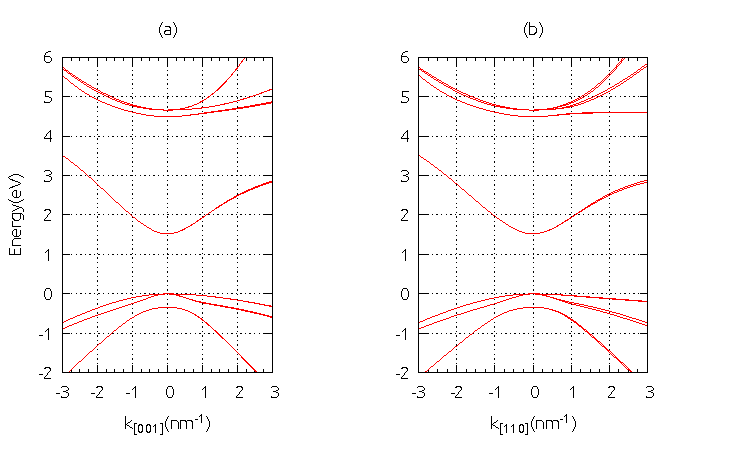
\includegraphics[width=0.70\textwidth]{./Figures/band-gaas.pdf}
%\rule{35em}{0.5pt}
\caption[computer kp 14-band GaAs]{Cấu trúc vùng năng lượng của chất bán dẫn GaAs bằng phương pháp kp $14\times14$ band, (a) $k\parallel[001]$ và (b) $k\parallel[110]$}
\label{fig:computer kp 14-band GaAs}
\end{figure}
Như chúng ta thấy ở ình 4.1 a thì độ tách mức năng lượng ở vùng hóa trị j=3/2 có độ tách không rõ ràng như ở hình b, còn đối với chất bán dẫn  GaInAs thì ngược lại ta thấy ở vùng hóa trị hình như ở hình a và b không có khác nhau cho lắm, còn ở vùng dẫn thì có sự khác nhau rõ ràng.
\begin{figure}[ht]
\centering
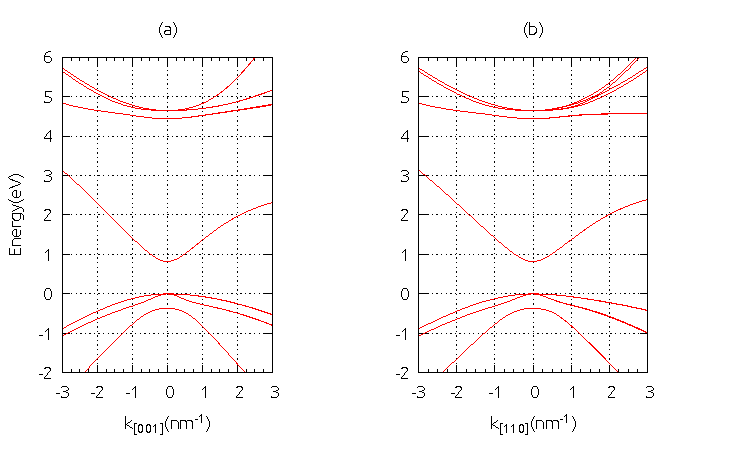
\includegraphics[width=0.70\textwidth]{./Figures/band-GaInAs.pdf}
%\rule{35em}{0.5pt}`
\caption[computer kp 14-band GaInAs]{Cấu trúc vùng năng lượng của chất bán dẫn GaInAs bằng phương pháp kp $14\times14$ band, (a) $k\parallel[001]$ và (b) $k\parallel[110]$}
\end{figure}

%\begin{figure}[ht]
%\centering
%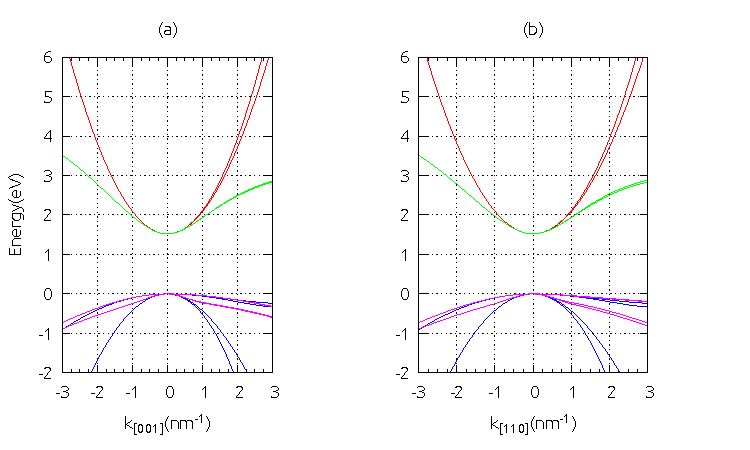
\includegraphics[width=0.70\textwidth]{./Figures/band14+lowdin.pdf}
%%\rule{35em}{0.5pt}
%\caption[computer kp 14-band and L$\ddot{o}$wdin GaAs]{Cấu trúc vùng năng lượng của chất bán dẫn GaAs bằng phương pháp kp $14\times14$ band màu xanh đậm và xanh dương(4-band đầu tiên của vùng hóa trị) và phương pháp L$\ddot{o}$wdin màu đỏ và tím(2 band đầu tiên của vùng dẫn), (a) $k\parallel[001]$ và (b) $k\parallel[110]$ }
%\end{figure}
\begin{figure}[ht]
\centering
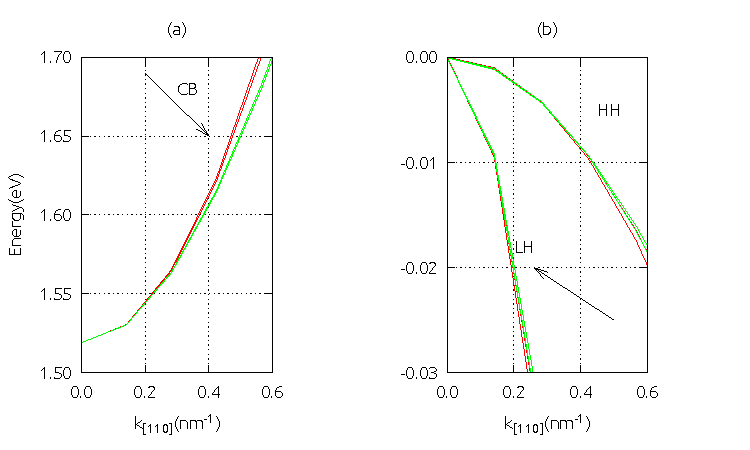
\includegraphics[width=0.70\textwidth]{./Figures/comparsion.pdf}
%\rule{35em}{0.5pt}
\caption[computer kp 14-band and L$\ddot{o}$wdin GaAs]{Cấu trúc vùng năng lượng của chất bán dẫn GaAs được tính bằng 2  phương pháp: kp $14\times14$ band màu xanh và L$\ddot{o}$wdin band  màu đỏ, (a) Độ phân tán của dãy dẫn và (b) Độ phân tán của dãy hóa trị}
\end{figure}
\begin{figure}[ht]
\raggedleft
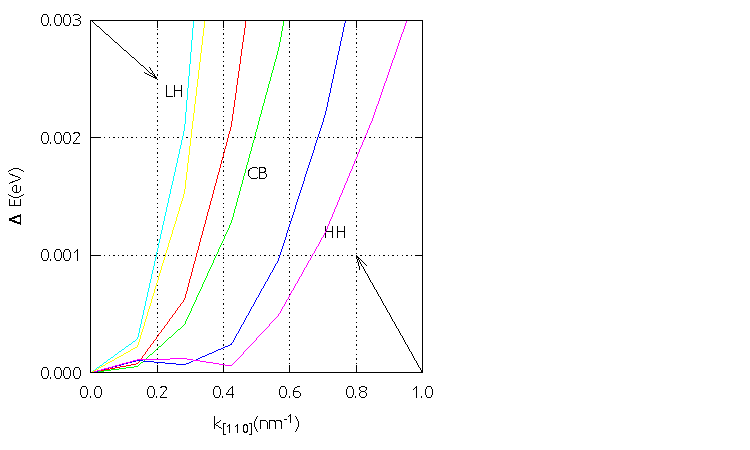
\includegraphics[width=0.70\textwidth]{./Figures/comparsion2.pdf}
%\rule{35em}{0.5pt}
\caption[so sánh phương pháp kp 14-band GaAs và L$\ddot{o}wdin$]{Độ tách suy biến của mức năng lượng spin up và spin down\\
 $\Delta E(k_{[110]})= \vert\Delta E(k_{[110]}.\uparrow) - \Delta E(k_{[110]}.\downarrow)\vert$}
\end{figure}
\chapter{\bfseries Giếng Lượng Tử}
\label{Chapter4} %
Hàm sóng của điện tử trong giếng lượng tử có dạng sau:
\begin{equation}
\psi^{\alpha}(\mathbf{r})=\sum_{i=1}^{l_{\alpha}=14} F_i^{\alpha}(\mathbf{r})u_{i,k=0}(\mathbf{r})
\end{equation}
ở đây $u_{i,k=0}(\mathbf{r})$ là một hàm tuần hoàn với chu kỳ là hằng số mạng của tinh thể hệ số $\alpha=c,l_c=1\dots8$ tương ứng với vùng dẫn, $\alpha=v,l_v=9\dots 14$ tương ứng với vùng hóa trị  và $F_i^{\alpha}(\mathbf{r})$ là bao gồm tất cả các thành phần hàm envelope trong gần đúng envelope đôi khi người ta gọi là gần đúng khối lượng hiệu dụng ta có phương trình sau đây [8]:
\begin{equation}
\sum_{i=1}^{l_{\alpha}=14}\left[\mathcal{H}_{ij}^{\alpha}\left(-i\nabla\right) +V_i\left(\mathbf{r}\right)\delta_{ij}\right]F_i^{\alpha}(\mathbf{r})=E^{\alpha}F_j^{\alpha}(\mathbf{r})
\end{equation}
ở dây $H(\mathbf{k})$ là chuẩn Hamiltonian khối lượng hiệu dụng, $V_i\left(\mathbf{r}\right)$ là thế của giếng lượng tử nếu ta chọn trục lượng tử hóa theo trục $z\parallel[001]$ trong tinh thể thì ta có dạng sau, nói thêm thế $V_i\left(\mathbf{r}\right)$ có thể hiểu là khi 2 vật liệu đặt sát vào nhau thi sẽ có một lớp tiếp xúc giữa chúng có thể tại ra những điểm kỳ dị và dán đoạn của  dãy năng lượng và ta có thể tổng quát hóa nó thành một thế năng trong trường hợp này là thế năng của giếng lượng tử: 
\begin{align}
\mathcal{H}_{ij}^{\alpha}\left(-i\nabla\right)=\mathcal{H}_{ij}^{\alpha}\left(k_x,k_y,-i(\partial / \partial z)\right)=\mathcal{H}_{ij}^{\alpha}\left(k_{\parallel},-i(\partial / \partial z)\right)\notag \\
V_i\left(\mathbf{r}\right)=V_i\left(\mathbf{z}\right),\qquad F_j^{\alpha}(\mathbf{r})=e^{ik_{\parallel}r_{\parallel}}\Phi_i^{\alpha}(z)=e^{ik_xx}e^{ik_yy}\Phi_i^{\alpha}(z)
\end{align}
do đó ta viết lại phương trình trên lại như sau:
\begin{equation}
\sum_{i=1}^{14}\left[\mathcal{H}_{ij}^{\alpha}\left(k_{\parallel},-i(\partial / \partial z)\right) +V_i(\mathbf{r})\delta_{ij}\right]F_i^{\alpha ,k_{\parallel}}(\mathbf{r})=E^{\alpha ,k_{\parallel}}F_j^{\alpha ,k_{\parallel}}(\mathbf{r})
\end{equation}

Để giải phương trình (5.4) chúng ta cần phải tìm dạng của hàm envelope và điều kiện biên, một câu hỏi đặt ra điều kiện như thế nào là thích hợp ở đây tôi tham khảo [14,18]:
\begin{equation}
\hat{k}_zh(z)\longrightarrow -\frac{i}{2}\left(\frac{\partial}{\partial z}h(z) + h(z)\frac{\partial}{\partial z}\right), \qquad \hat{k}_z^2 \longrightarrow -\frac{\partial}{\partial z}h(z)\frac{\partial}{\partial z}
\end{equation}	  
còn hàm envelope có thể triển khai theo sóng phẳng như sau [6,7,8]
\begin{equation}
F_i^{\alpha,k_{\parallel}} = \sum_{l=1}^N a_{i,l}^{{\alpha},k_{\parallel}}\phi_l(z)
\end{equation}
với 
\begin{equation}
\phi_i\left(z\right) =  \begin{cases}
\sqrt{\frac{2}{L_z}}\sin\left[\frac{i\pi}{L_z}\left(z +\frac{L_z}{2}\right)\right] &\qquad\text{nếu} -\frac{L_z}{2}\le z\le \frac{L_z}{2}\\
0 &\qquad\text{các trường hợp còn lại}
\end{cases}
\end{equation}
ở đây $L_z$ là hằng số và nó thường được chọn sao cho lớn hơn nhiều lần so với bề dày của giếng lượng tử, thây biểu thức (5.6) vào (5.4) đồng thời nhân bên trái hai vế với đại lượng $\phi^{*}$ và chuẩn hóa nó theo $z$ ta có một hệ ma trận $14N\times 14N$
\begin{equation}
\sum_{i=1}^{14}\sum_{l=1}^{N}\langle \phi_{l} \vert \mathcal{H}_{ij} +V_i\delta_{ij}\vert \phi_{l^{'}} \rangle a_{il}^{\alpha,k_{\parallel}} = E^{\alpha,k_{\parallel}} a_{j
l^{'}}^{\alpha,k_{\parallel}}
\end{equation}
\section{Ứng dụng của giếng lượng tử}
Sau khi ta giải phương trình trên ta sẽ có cấu trúc năng lượng của chất bán dẫn trong giếng lượng tử, có các mức năng lượng ta có thể tính được nồng độ hạt tải của điện tử, lỗ trống, cũng như độ phân cực$\dots$ ta hãy xét Hamiltonian toàn phần của  hệ điện tử trong các dãy tương tác với ánh sáng (many-body system) có dạng sau [11,12,13,14,15]:   
\begin{equation}
\mathcal{H} = \mathcal{H}_{band \;structure} +\mathcal{H}_{light\;matter} +\mathcal{H}_{coulomb}
\end{equation}
trong đó $\mathcal{H}_{band\;structure}$ là Hamiltonian của hệ điện tử trong các dãy\footnote{Ở đây ta cần lưu ý rằng điệnt ử trong dãy hóa trị có phổ năng lượng âm, do đó nó cũng có một khối lượng $m_{\lambda=v <0}$, để tránh vấn đề khối lượng âm ta đưa ra khái niệm lổ trống như một giả hạt mới có điện tích dương và khối lương  $m_h= -m_v$. Sự tương đương về mặt vật lý của lổ trống và điện tử trong dãy hóa trị được giải thích như sau: Khi chưa có kích thích tất cả các điện tử trong chất bán dẫn sẽ lấp đầy tất cả các mức năng lượng của hóa trị, khi có kích thích một điện tử ở vùng hóa trị sẽ nhãy lên vùng dẫn và để lại trong dãy hóa trị một chỗ trống trong phổ năng lượng gây ra bởi quá trình hấp thụ lấp-bỏ chổ trống giữa các điện tử ở vùng hóa trị còn lại, có nghĩa là một điện tử ở vùng hóa trị bất kỳ sẽ có khả năng bỏ vị trí lấp đầy của nó để lấp đầy chổ trống vừa được tạo ra bởi một điện tử khác, lập lại quá trình đối với lỗ trống mới $\dots$ Và như vậy ta có một quá trình song song giửa chổ trống và các điện tử hóa trị, khi đó ta dồng nhất vai trò của một điện tử hóa trị bằng khái niệm lổ trống với tư cách là giả hạt mô tả chuyển dộng của chổ trống năng lượng trong dãy hóa trị Sự tương phản giửa lổ trống và điện tử ở vùng hóa trị cho phép ta xem lỗ trống như một giả hạt thật sự với khối lượng dương, điện tích dương. trong điều kiện cân bằng xác xuất để tìm thấy một lổ trống trong trạng thái k được cho bởi 
\(n_{h,k}= 1-n_{v,k}\) , có nghĩa là việc tìm thấy một lổ trống ở trạng thái k đồng nghĩa với việc mất đi một điện tử hóa trị trong trạng thái tương ứng },$\mathcal{H}_{light\;matter}$ là Hamiltonian tương ứng với tương tác của điện tử với trường ngoài và $\mathcal{H}_{coulomb}$ là Hamiltonian của thế Coulomb, trong  biễu diễn lượng tử hóa lần hai chúng có dạng sau đây:
\begin{align}
\mathcal{H}_{band\;structure} &= \sum_{\lambda,k_{\parallel}}E_{k_{\parallel}}^{\lambda}a_{\lambda k_{\parallel}}^{\dagger}a_{\lambda k_{\parallel}}\notag\\
\mathcal{H}_{light\;matter} &= \frac{e}{m_0}\mathcal{A}(t)P=\frac{e}{m_0}\mathcal{A}(t)\sum_{\lambda\lambda^{'}k_{\parallel}}\Pi_{k_{\parallel}}^{\lambda\lambda^{'}}
a_{\lambda k_{\parallel}}^{\dagger}a_{\lambda k_{\parallel}}
\end{align} 
chú ý ở trên ta đâ bỏ đi số hạng $\frac{e\mathcal{A}^2}{2m}$ xem [15,16] hoặc ở phụ lục, ở đây $\mathcal{A}(t)$ là thế véctơ của trường ánh sáng,$a_{\lambda k_{\parallel}}^{\dagger},a_{\lambda k_{\parallel}}$  lần lượt là toán tử sinh và  toán tử hủy, $\Pi_{k_{\parallel}}^{\lambda\lambda^{'}}$ là thành phần ma trận động lượng trong trường hợp này là ma trận động lượng $14\times14$ kp và nó có giá trị sau đây
\begin{equation}
\Pi_{k_{\parallel}}^{\lambda\lambda^{'}} = \int dz\sum_{nm}f_{nk_{\parallel}}^{\lambda *}(z)\pi_{nm}(k_{\parallel},-i\partial
_z)f_{mk_{\parallel}}^{\lambda^{'}}(z)
\end{equation}
với $\pi_{nm}=\frac{m_0}{\hbar}P_{nm}=\frac{m_0}{\hbar}\nabla_{k}\mathcal{H}_{nm}(k)$ và ta cần chú rằng $\mathcal{H}\propto\frac{e}{m_0}\mathcal{A}\mathbf{P}\propto\mathbf{r}\mathbf{E}$ do đó ta có thể biểu diễn $\mathcal{H}_{light\;matter}$ theo thế véctơ hoặc điện trường trong bài báo cáo này tôi sử dụng thế véctơ, còn thành phần Hamiltonian Coulomb trong multi-subband giếng lượng tử có dạng sau đây:
\begin{equation}
\mathcal{H}_{Coulomb}= \frac{1}{2}\sum_{\lambda_1\lambda_2\lambda_3\lambda_4 k_{\parallel}k_{\parallel}^{'}q_{\parallel}}
V_{k_{\parallel}k_{\parallel}^{'}q_{\parallel}}^{\lambda_1\lambda_2\lambda_3\lambda_4}
\times a_{\lambda_1 k_{\parallel} +q_{\parallel}}^{\dagger}a_{\lambda_2 k_{\parallel}^{'}-q_{\parallel}}^{\dagger}a_{\lambda_3 k_{\parallel}^{'}}a_{\lambda_4 k_{\parallel}}
\end{equation}
ở đây thành phần ma trận thế Coulomb thuộc nhiều dãy trong giếng lượng tử được cho bởi dạng sau [17]
\begin{equation}
V_{k_{\parallel}k_{\parallel}^{'}q_{\parallel}}^{\lambda_1\lambda_2\lambda_3\lambda_4}
=\frac{e^2}{2\epsilon\epsilon_0 L^2|q_{\parallel}|}\int dz_1\int dz_2
e^{-|q_{\parallel}||z_2-z_1|}\times\sum_{m} f_{mk_{\parallel}+q_{\parallel}}^{\lambda_1 *}(z_1)
f_{mk_{\parallel}}^{\lambda_4}(z_1)
\sum_{n}f_{nk_{\parallel}^{'}-q_{\parallel}}^{\lambda_2 *}(z_2)
f_{nk_{\parallel}^{'}}^{\lambda_3}(z_2) 
\end{equation}
để dẫn ra phương trình chuyển động cho hàm phân bố điện tử, lổ trống và hàm phân cực (thể hiện mối tương quan giữa cặp điện tử ở vùng dẫn và lổ trống ở vùng hóa trị), ta sử dụng phương trình chuyển động của các toán tử của Heisenberg sau đó ta lấy trị trung bình ta sẽ có kết quả cần tìm, ta hãy tìm nó thử xem có đạng như thế nào, như ta đã biết phương trình chuyển động Heisenberg có dạng sau:
\begin{equation}
\frac{d}{dt}\langle \mathcal{A}\rangle = \frac{i}{\hbar}\langle[\mathcal{H},\mathcal{A}]\rangle
\end{equation}
dấu $\langle\rangle$ được hiểu là lấy trị trung bình, ta xét đại lượng sau $\chi_{k_{\parallel}}^{\lambda\lambda^{'}}=\langle a_{\lambda k_{\parallel}}^{\dagger}a_{\lambda^{'} k_{\parallel}}\rangle$, ở đây $\lambda,\lambda^{'}$ lần lượt là chỉ số $c,c^{'}$ nếu ở vùng dẫn, $v,v^{'}$ nếu ở vùng hóa trị , nếu ta xét trường hợp $\lambda=\lambda^{'}$ thì ta sẽ có các đại lượng như $n_{k_{\parallel}}^{c} = \langle a_c^{\dagger}a_c\rangle,n_{k_{\parallel}}^{v} = \langle a_v^{\dagger}a_v\rangle$ tương ứng là nồng độ hạt tải của điện tử và lỗ trống và nó thể hiện tính chất dẫn điện, nếu ta xét trường hợp $\lambda\neq\lambda^{'}$ thì ta cũng có các đại lượng $n_{k_{\parallel}}^{cc^{'}} = \langle a_c^{\dagger}a_{c^{'}}\rangle,n_{k_{\parallel}}^{vv^{'}} = \langle a_v^{\dagger}a_{v^{'}}\rangle$ cho biết thông tin tương quan của hai dãy dẫn hoặc hai dãy hóa trị kề cận với nhau, còn đại lượng $\rho^{vc}$ là đại lượng phân cực thể hiện mối tương quan giữa điện tử và lỗ trống.\\
Khi tính toán với các toán tử sinh, hủy ta sử dụng các hệ thức sau đây:
\begin{align}
&[a_i,a_j^{\dagger}]= \delta_{ij},\qquad[a_i,a_j]=[a_i^{\dagger},a_j^{\dagger}]=0 \qquad (boson)\notag\\
&\{a_i,a_j^{\dagger}\}= \delta_{ij},\qquad \{a_i,a_j\}=\{a_i^{\dagger},a_j^{\dagger}\}=0 \qquad (fermion)\notag\\
&[b_v^{\dagger}b_v,b_r] =-b_v\delta_{vr},\qquad [b_v^{\dagger}b_v,b_r^{\dagger}]=b_v^{\dagger}\delta_{vr}\notag\\
&[AB,C]=A[B,C] +[A,C]B,\notag\\
&[A,BC]=[A,B]C+B[A,C],\notag\\
&[AB,C]=A\{B,C\}-\{A,C\}B
\end{align}
thây biểu thức Hamiltonian (5.9) và $\chi_{k_{\parallel}}^{\lambda\lambda^{'}}=\langle a_{\lambda k_{\parallel}}^{\dagger}a_{\lambda^{'} k_{\parallel}}\rangle$ vào phương trình chuyển động (5.14) ta có
\begin{equation}
\frac{\partial}{\partial t}\chi_{k_{\parallel}}^{\lambda\lambda^{'}} =\frac{i}{\hbar}\langle[\mathcal{H}_{band \;structure} +\mathcal{H}_{light\;matter} +\mathcal{H}_{coulomb},a_{\lambda k_{\parallel}}^{\dagger}a_{\lambda^{'} k_{\parallel}^{'}}]\rangle
\end{equation}
xét số hạng thứ nhất 
\begin{align}
&\frac{i}{\hbar}\biggl[\mathcal{H}_{band \;structure},a_{\lambda k_{\parallel}}^{\dagger}a_{\lambda^{'} k_{\parallel}^{'}}\biggr]=\frac{i}{\hbar}\sum_{\mu k_{\parallel}}E_{k_{\parallel}}^{\mu}\biggl[a_{\mu k_{\parallel}}^{\dagger}a_{\mu k_{\parallel}},a_{\lambda k_{\parallel}}^{\dagger}a_{\lambda^{'} k_{\parallel}^{'}}\biggr]\notag\\
&=\frac{i}{\hbar} \sum_{\mu k_{\parallel}}E_{k_{\parallel}}^{\mu}
\left(\biggl[a_{\mu k_{\parallel}}^{\dagger}a_{\mu k_{\parallel}},a_{\lambda k_{\parallel}}^{\dagger}\biggr]a_{\lambda^{'} k_{\parallel}^{'}}
+a_{\lambda k_{\parallel}}^{\dagger}\biggl[a_{\mu k_{\parallel}}^{\dagger}a_{\mu k_{\parallel}},a_{\lambda^{'} k_{\parallel}^{'}}
\biggr] \right)\notag\\
&=\frac{i}{\hbar} \sum_{\mu k_{\parallel}}E_{k_{\parallel}}^{\mu}\left(
\delta_{\mu\lambda}\delta_{k_{\parallel}k_{\parallel}} a_{\mu k_{\parallel}}^{\dagger}a_{\lambda^{'}k_{\parallel}^{'}}
-\delta_{\mu \lambda^{'}}\delta_{k_{\parallel}k_{\parallel}^{'}}a_{\lambda k_{\parallel}}^{\dagger}a_{\mu k_{\parallel}^{'}}
\right)\notag\\
&=\frac{i}{\hbar}\left( \underbrace
{\sum_{\mu k_{\parallel}}E_{k_{\parallel}}^{\mu}
\delta_{\mu\lambda}\delta_{k_{\parallel}k_{\parallel}}a_{\mu k_{\parallel}}^{\dagger}a_{\lambda^{'}k_{\parallel}^{'}}}_{\mu =\lambda}
- \underbrace{\sum_{\mu k_{\parallel}}E_{k_{\parallel}}^{\mu}\delta_{\mu \lambda^{'}}\delta_{k_{\parallel}k_{\parallel}^{'}}a_{\lambda k_{\parallel}}^{\dagger}a_{\mu k_{\parallel}^{'}}}_{\mu=\lambda^{'},k_{\parallel}=k_{\parallel}^{'}}
\right)\notag\\
&=\frac{i}{\hbar} \left(E_{k_{\parallel}}^{\lambda}
 a_{\lambda k_{\parallel}}^{\dagger}a_{\lambda^{'}k_{\parallel}}
-E_{k_{\parallel}}^{\lambda^{'}} a_{\lambda k_{\parallel}}^{\dagger}a_{\lambda^{'} k_{\parallel}}
\right) = \frac{i}{\hbar} a_{\lambda k_{\parallel}}^{\dagger}a_{\lambda^{'} k_{\parallel}}\left(E_{k_{\parallel}}^{\lambda}-E_{k_{\parallel}}^{\lambda^{'}} \right)
\end{align}
xét số hạng thứ hai
\begin{align}
&\frac{i}{\hbar}\biggl[\mathcal{H}_{light \;matter},a_{\lambda k_{\parallel}}^{\dagger}a_{\lambda^{'} k_{\parallel}^{'}}\biggr]=\frac{i}{\hbar}\frac{e}{m_0}\mathcal{A}(t)\sum_{\mu\mu^{'}k_{\parallel}}\Pi_{k{\parallel}}^{\mu\mu^{'}}
\biggl[
a_{\mu k_{\parallel}}^{\dagger}a_{\mu^{'} k_{\parallel}},a_{\lambda k_{\parallel}}^{\dagger}a_{\lambda^{'} k_{\parallel}^{'}}\biggr]\notag\\
&=\frac{i}{\hbar}\frac{e}{m_0}\mathcal{A}(t)\sum_{\mu\mu^{'}k_{\parallel}}\Pi_{k{\parallel}}^{\mu\mu^{'}}
\biggl[a_{\mu k_{\parallel}}^{\dagger}a_{\mu^{'} k_{\parallel}},a_{\lambda k_{\parallel}}^{\dagger}\biggr]a_{\lambda^{'} k_{\parallel}^{'}} + 
a_{\lambda k_{\parallel}}^{\dagger}\biggl[a_{\mu k_{\parallel}}^{\dagger}a_{\mu^{'} k_{\parallel}},a_{\lambda^{'} k_{\parallel}^{'}}\biggr]\notag\\
&=\frac{i}{\hbar}\frac{e}{m_0}\mathcal{A}(t)\sum_{\mu\mu^{'}k_{\parallel}}\Pi_{k{\parallel}}^{\mu\mu^{'}}
\left(
a_{\mu k_{\parallel}}^{\dagger}\{a_{\mu^{'} k_{\parallel}},a_{\lambda k_{\parallel}}^{\dagger}\}a_{\lambda^{'}k_{\parallel}^{'}}-
a_{\lambda k_{\parallel}}^{\dagger}\{a_{\mu k_{\parallel}}^{\dagger}a_{\lambda^{'}k_{\parallel}^{'}}\}a_{\mu^{'} k_{\parallel}}
\right)\notag\\
&=\frac{i}{\hbar}\frac{e}{m_0}\mathcal{A}(t)\sum_{\mu\mu^{'}k_{\parallel}}\Pi_{k{\parallel}}^{\mu\mu^{'}}
\left(
a_{\mu k_{\parallel}}^{\dagger}a_{\lambda^{'}k_{\parallel}^{'}}\delta_{\mu^{'}\lambda}
\delta_{k_{\parallel}k_{\parallel}} -
a_{\lambda k_{\parallel}}^{\dagger}a_{\mu^{'} k_{\parallel}}\delta_{\lambda^{'}\mu}\delta_{k_{\parallel}k_{\parallel}^{'}}
\right)\notag\\
&=\frac{i}{\hbar}\frac{e}{m_0}\mathcal{A}(t)\sum_{\mu k_{\parallel}}\Pi_{k{\parallel}}^{\mu\lambda}a_{\mu k_{\parallel}}^{\dagger}a_{\lambda^{'}k_{\parallel}}
-\frac{i}{\hbar}\frac{e}{m_0}\mathcal{A}(t)\sum_{\mu^{'}k_{\parallel}}\Pi_{k{\parallel}}^{\lambda^{'}\mu^{'}}
a_{\lambda k_{\parallel}}^{\dagger}a_{\mu^{'} k_{\parallel}}\notag\\
&=\frac{i}{\hbar}\frac{e}{m_0}\mathcal{A}(t)\sum_{\mu k_{\parallel}}\Pi_{k{\parallel}}^{\mu\lambda}a_{\mu k_{\parallel}}^{\dagger}a_{\lambda^{'}k_{\parallel}}
-\frac{i}{\hbar}\frac{e}{m_0}\mathcal{A}(t)\sum_{\mu k_{\parallel}}\Pi_{k{\parallel}}^{\lambda^{'}\mu}
a_{\lambda k_{\parallel}}^{\dagger}a_{\mu k_{\parallel}}\notag\\
&=\frac{i}{\hbar}\frac{e}{m_0}\mathcal{A}(t)\sum_{\mu k_{\parallel}}\Pi_{k{\parallel}}^{\mu\lambda}\chi_{k_\parallel}^{\mu\lambda^{'}}
-\frac{i}{\hbar}\frac{e}{m_0}\mathcal{A}(t)\sum_{\mu k_{\parallel}}\Pi_{k{\parallel}}^{\lambda^{'}\mu}
\chi_{k_{\parallel}}^{\lambda\mu}
\end{align}
số hạng tương tác thế Coulomb còn lại ta tính tương tự và chú ý rằng ta sẽ sử dụng kết quả gần đúng ở mục (2.9) ta có số hạng thứ ba như sau:
\begin{align}
\frac{i}{\hbar}\biggl[\mathcal{H}_{Coulomb},a_{\lambda k_{\parallel}}^{\dagger}a_{\lambda^{'} k_{\parallel}^{'}}\biggr]
&=\frac{i}{\hbar}\frac{e}{m_0}\sum_{\mu\mu_1\nu q}
V_{k_{\parallel}}^{\mu_1\lambda^{'}\nu\mu}\chi_{k_{\parallel}+q_{\parallel}}
^{\mu_1\nu}\chi_{k_{\parallel}}^{\lambda\mu}\notag\\
&- \frac{i}{\hbar}\frac{e}{m_0}\sum_{\mu\mu_1\nu q}
V_{k_{\parallel}}^{\mu_1\mu\nu\lambda}\chi_{k_{\parallel}+q_{\parallel}}
^{\mu_1\nu}\chi_{k_{\parallel}}^{\mu\lambda^{'}}
+\frac{\partial}{\partial t}\chi_{k_{\parallel}}^{\lambda\lambda^{'}}\Bigl\vert_{coll}
\end{align}
thây các giá trị (5.17),(5.18),(5.19) vào phương trình (5.16) ta có dạng tổng quát sau đây:
\begin{align}
\frac{\partial}{\partial t}\chi_{k_{\parallel}}^{\lambda\lambda^{'}}=
\frac{i}{\hbar}\left(E_{k_{\parallel}}^{\lambda} - E_{k_{\parallel}}^{\lambda^{'}}\right)\chi_{k_{\parallel}}^{\lambda\lambda^{'}} +\frac{i}{\hbar}\sum_{\mu}
\left[
\Omega_{k_{\parallel}}^{\mu\lambda}\chi_{k_{\parallel}}^{\mu\lambda^{'}} -
\Omega_{k_{\parallel}}^{\lambda^{'}\mu}\chi_{k_{\parallel}}^{\lambda\mu}
\right]
+\frac{\partial}{\partial t}\chi_{k_{\parallel}}^{\lambda\lambda^{'}}\Bigl\vert_{coll}
\end{align}	
trong đó 
\begin{equation}
\Omega_{k_{\parallel}}^{\lambda\lambda^{'}}=\frac{e}{m_0}\mathcal{A}(t).\Pi_{k_{\parallel}}^{\lambda\lambda^{'}} -\sum_{\mu\nu q_{\parallel}}
V_{k_{\parallel},k_{\parallel}+q_{\parallel},q_{\parallel}}^{\mu\lambda\nu\lambda^{'}}
\chi_{k_{\parallel}+q_{\parallel}}^{\mu\nu}
\end{equation}
khi $\lambda\neq\lambda^{'}$ thì đại lượng $\Omega_{k_{\parallel}}^{\lambda\lambda^{'}}$ được gọi là tần số tái chuẩn hóa Rabi, còn khi $\lambda = \lambda^{'}$ được gọi là năng lượng chuẩn hóa của dãy năng lượng và đại lượng $\frac{\partial}{\partial t}\chi_{k_{\parallel}}^{\lambda\lambda^{'}}\Bigl\vert_{coll}$ 	được gọi là số hạng mô tả qua chạm hoặc tán xạ được tính gần đúng trong thời gian khử pha.
\begin{figure}[hc]
\centering
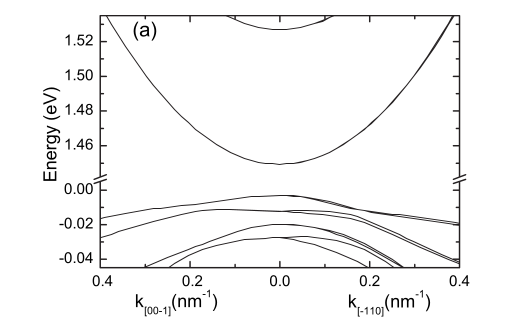
\includegraphics[width=0.70\textwidth]{./Figures/well1.png}
\caption[cấu trúc vùng năng lượng trong quantum well]{Cấu trúc vùng năng lượng của chất bán dẫn $GaAs/Al_{0.35}Ga_{0.65}As$ trong giếng lượng tử với bờ rộng là 12.nm với trục $k_{[110]}$ Ref[16]}
\end{figure}
\section{Dòng spin và dòng điện tích}
Sau khi giải phương trình trên ta sẽ có các đại lượng $n_{k_{\parallel}}^{cc},n_{k_{\parallel}}^{vv}$ tương ứng với nồng độ (mật độ)  hạt tải của điện tử và lổ trống (population), còn các đại lượng $n_{k_{\parallel}}^{cc^{'}},n_{k_{\parallel}}^{vv^{'}}$ cũng thể hiện mối tương quan của 2 dãy kề cận với nhau (intersubband coherences) và cuối cùng là đại lượng $\rho_{k_\parallel}^{cv}$ là đại lượng phân cực thể hiện mối tương quan của điện tử và lổ trống. Như ta đã biết dòng điện được định nghĩ như sau:
\begin{equation}
\mathbf{J}^{pop}(t) =nqv=\frac{e}{m_0}\sum_{c,k_{\parallel}}\Pi_{k_{\parallel}}^{cc}n_{k_{\parallel}}^{cc} +
\frac{e}{m_0}\sum_{v,k_{\parallel}}\Pi_{k_{\parallel}}^{vv}n_{k_{\parallel}}^{vv}
\end{equation}
dòng này tôi gọi là dòng population, còn dòng intersubband coherences được định nghĩa như sau:
\begin{equation}
\mathbf{J}^{coh}(t) =nqv=\frac{e}{m_0}\sum_{c\neq c^{'},k_{\parallel}}\Pi_{k_{\parallel}}^{cc^{'}}n_{k_{\parallel}}^{cc^{'}} +
\frac{e}{m_0}\sum_{v\neq v^{'},k_{\parallel}}\Pi_{k_{\parallel}}^{vv^{'}}n_{k_{\parallel}}^{vv^{'}}
\end{equation}
Tương tự ta định nghĩa dòng spin population và spin coherent như sau theo hướng $i=x,y,z$, ta có dòng spin population như sau: 
\begin{equation}
\mathbf{S}^{pop}(t) = \frac{\hbar}{m_0}\sum_{c,\mathbf{k}_\parallel}
{\displaystyle\mathsmaller{\mathsmaller{\sum\nolimits_{i\mathbf{k}_\parallel}^{cc}}}}
\Pi_{k_{\parallel}}^{cc}n_{k_{\parallel}}^{cc} +
\frac{\hbar}{m_0}\sum_{v,\mathbf{k}_\parallel}
{\displaystyle\mathsmaller{\mathsmaller{\sum\nolimits_{i\mathbf{k}_\parallel}^{vv}}}}
\Pi_{k_{\parallel}}^{vv}n_{k_{\parallel}}^{vv}
\end{equation}
và dòng spin coherent như sau:
\begin{equation}
\mathbf{S}^{coh}(t) = \frac{\hbar}{m_0}\sum_{c\neq c^{'},\mathbf{k}_\parallel}
{\displaystyle\mathsmaller{\mathsmaller{\sum\nolimits_{i\mathbf{k}_\parallel}^{cc^{'}}}}}
\Pi_{k_{\parallel}}^{cc^{'}}n_{k_{\parallel}}^{cc^{'}} +
\frac{\hbar}{m_0}\sum_{v\neq v^{'},\mathbf{k}_\parallel}
{\displaystyle\mathsmaller{\mathsmaller{\sum\nolimits_{i\mathbf{k}_\parallel}^{vv^{'}}}}}
\Pi_{k_{\parallel}}^{vv^{'}}n_{k_{\parallel}}^{vv^{'}}
\end{equation}
hình chiếu thành phần i của spin lên các trục $x,y,z$ được miêu tả bởi thành phần ma trận mômen động lượng như sau [22,16]:
\begin{equation}
{\mathsmaller{\sum\nolimits_{i\mathbf{k}_\parallel}^{cc^{'}}}} =
\frac{1}{2}\int dz\sum_{mn}
f_{m\mathbf{k}_{\parallel}}^{c*}(z)
\boldsymbol{\sigma}_i
f_{n\mathbf{k}_{\parallel}}^{c^{'}}(z)
\end{equation}
và 
\begin{equation}
{\mathsmaller{\sum\nolimits_{i\mathbf{k}_\parallel}^{vv^{'}}}} =
\frac{1}{2}\int dz\sum_{mn}
f_{m\mathbf{k}_{\parallel}}^{v*}(z)
\boldsymbol{\mathcal{J}}_i
f_{n\mathbf{k}_{\parallel}}^{v^{'}}(z)
\end{equation}
ở đây $\boldsymbol{\sigma}_i$ là ma trận Pauli, còn $\boldsymbol{\mathcal{J}}_i$ là ma trận với spin bằng $j=-3/2$. sau khi ta có các đại lượng dòng spin và dòng điện tích của các trường hợp coherent và population ta định nghĩa đại lượng tổng của hai dòng này như:\\
Tổng dòng điện tích của điện tử hoặc lổ trống đống góp vào dòng injection như sau:
\begin{equation}
\mathbf{J}(t) =\mathbf{J}^{pop}(t) +\mathbf{J}^{coh}(t)
\end{equation}
còn tổng dòng spin của điện tử hoặc lổ trống đống góp vào dòng injection như sau:
\begin{equation}
\mathbf{S}(t) = \mathbf{S}^{pop}(t) + \mathbf{S}^{coh}(t)
\end{equation}
Việc tính tổng cả hai dòng này rất khó khăn, thường thì ta sẽ làm bố trí thí nghiệm sao cho triệt tiêu một dòng và dòng còn lại ta sẽ tính đơn giản 
\chapter{Kết Luận- Hướng Phát Triển Đề Tài}
\label{Chapter0} % For referencing the chapter elsewhere, use \ref{Chapter1} 
\rhead{\bfseries Khóa Luận Tốt Nghiệp,Năm 2013}
\section{Kết Luận}
Trên đây tôi đã trình bày phương pháp tính toán cấu trúc vùng năng lượng của chất bán dẫn bằng phương pháp kp $14\times14$ chính xác và trong gần đúng nhiễu loạn L$\ddot{o}$wdin.
Sau khi có được năng lượng thì tôi đã ứng dụng nó vào phương trình Bloch bán dẫn để tìm dòng điện tích, dòng spin cũng như độ phân cực do giới hạn về thời gian làm khóa luận cũng như công cụ tính toán nên kết quả về dòng spin, dòng điện tích chưa được mô phỏng hóa qua dữ liệu.
\section{Hướng phát triển đề tài}
Tôi sẽ tiếp tục phát triển giải bài toán trong trường hợp có từ trường cũng như điện trường vào, và sẽ giải số phương trình (5.20) để tính các dòng, trong đó có các dòng đã có trong thực nghiệm đo khi xét từ trường ngoài vào ở hai bài báo sau: Magnetoelectric Photocurrent Generated by Direct Interband Transitions in InGaAs/InAlAs Two-Dimensional Electron Gas(PR.L 104, 246601 (2010)) và
Quadratic magnetic field dependence of magnetoelectric photocurrent (PR.B 83, 155307 (2011))



%----------------------------------------------------------------------------------------
%	THESIS CONTENT - APPENDICES
%----------------------------------------------------------------------------------------

\addtocontents{toc}{\vspace{2em}} % Add a gap in the Contents, for aesthetics
\appendix % Cue to tell LaTeX that the following 'chapters' are Appendices

% Include the appendices of the thesis as separate files from the Appendices folder
% Uncomment the lines as you write the Appendices


\chapter{Lý Thuyết Orbit Phân Tử} % Main appendix title
\label{AppendixA} % For referencing this appendix elsewhere, use \ref{AppendixA}
\lhead{Appendix A. \emph{Phụ lục}} % This is for the header on each page - perhaps a shortened title

 \section{Cơ sở và phương pháp}
 Ba nhà khoa học Hund-Mulliken-Lennard Jones là những người đặt nền tảng cho phương pháp orbit phân tử bằng cách mở rộng khái niệm orbit nguyên tử(hệ một hạt nhân nguyên tử) cho phân tử (hệ nhiều hạt nguyên tử)
 \begin{enumerate}
 \item Nếu trong nguyên tử, mỗi electron được miêu tả bằng một hàm sóng(orbit nguyên tử ta ký hiệu AO), thì trong phân tử, mỗi electron cũng được miêu tả  bằng một hàm sóng $\boldsymbol{\Psi}$(orbit phân tử ta ký hiệu MO), và xác xuất tìm thầy elecron trong một thể tích $\boldsymbol{dv}$ của phân tử là $\boldsymbol{\psi}^2 dv$ tương tự như trong nguyên tử
 \item Nếu trong mỗi orbit nguyên tử, electron được đặc trưng bằng một bộ số lượng tử:$\emph{n,l,m,s}$ và ta có AO với các tên $\emph{s,p,d,f...}$ thì trong mỗi orbit phân tử, electron cũng được đặt trưng bằng một số các bộ lượng tử  và ta có MO với các tên $\sigma, \pi, \delta,\phi$
 \item Nếu mỗi orbit nguyên tử ứng với một mức năng lượng xác đinh, thì mỗi orbit phân tử cũng tương ứng với một mức năng lượng xác định
 \item Việc điền electron vào AO tuân theo nguyên lý vững bền, nguyên lý Pauli quy tắc Hund, thì việc điền electron vào MO cũng phải tuân theo những quy tắc đó
 \item Từ các AO của các nguyên tử tham gia vào việc tạo thành các liên kết, người ta có thể suy ra MO của phân tử mới tạo thành bằng cách tổ hợp tuyến tính các AO ban đầu: n AO tổ hợp tuyến tính cho n MO và các AO được sử dụng phải thỏa mản các điều kiện sau:
 \begin{itemize}
 \item[1/] Có năng lượng gần bằng nhau
 \item[2/] Có mức độ xen phủ rõ rệt
 \item[3/] Có tính đối xứng giống nhau đối với trục nối tâm hai nguyên tử
 \end{itemize}
\end{enumerate}  
\section{Tổ hợp tuyến tính hai AO}
Ta khảo tổ hợp tuyến tính hai AO $\psi_a$ và $\psi_b$ của hai nguyên tử Hidro a và b trong ion-phân tử hidro $H^+_2$. Khi electron ở gần hạt nhân ta coi trường lực tác dụng vào electron chỉ là của hạt nhân a và trạng thái nó được mô tả bằng hàm sóng orbit:
\begin{equation}
\psi_a=\frac{1}{\sqrt{\pi}}e^{-r_a}
\end{equation}
Ngược lại khi electron ở gần hạt nhân nguyên tử b, trạng thái của nó được mô tả bằng hàm sóng orbit nguyên tử:
\begin{equation}
\psi_b=\frac{1}{\sqrt{\pi}}e^{-r_b}
\end{equation}
Tổ hợp tuyến tính của 2 hàm sóng trên lại với nhau và ta gọi nó làm sóng mô tả trạng thái electron của orbit phân tử(LCAO):
\begin{equation}
\psi_{MO}=c_a\psi_a + c_b\psi_b
\end{equation}
vì hai hàm sóng AO là đồng nhất với nhau nên chúng tham gia vào MO vói cùng đóng góp với nhau:
\begin{equation}
c^2_a=c^2_b \rightarrow c_a=\pm c_b
\end{equation}
như vậy vói hai phân tử $H^+_2$ ta có hai MO
\begin{equation}
 \psi_+ = c_+\left(\psi_a + \psi_b \right)  \qquad \psi_{\_}=c_{\_}\left(\psi_a -\psi_b\right)
\end{equation}
với $c_+$ và $c_\_$ là các thứa số chung ứng với tổ hợp cộng và tổ hợp trừ 
\begin{enumerate}
\item Ta có thể xác định $c_+$ và $c_\_$ từ điều kiện chuẩn hóa hàm sóng, với hàm sóng $\psi_+$:
\begin{equation}
1=\int_{\infty}\psi_+^2 dv=\int_{\infty}c_+^2\left(\psi_a +\psi_b\right)^2 dv=
c_+^2 \left[ \int_{\infty}\psi_a^2dv +  \int_{\infty}\psi_b^2dv + 2\int_{\infty}\psi_a \psi_b dv\right]
\end{equation}
các orbit của hàm $\psi_a$ và $\psi_b$ là chuẩn hóa tức $\int_{\infty}\psi_b^2dv=\int_{\infty}\psi_b^2dv=1$ và ta ký hiệu đại lượng S bằng tích phân $\int_{\infty}\psi_a \psi_bdv$ được gọi là tích phân phủ thây vào ta có
\begin{equation}
c_+ = \frac{1}{\sqrt{2(1+S)}} \qquad \text{vì S<<1 nên } 1+S\approx 1, \text{do đó} \qquad c_+=\frac{1}{\sqrt{2}}
\end{equation}
kết quả cuối cùng ta có
\begin{equation}
\psi_+=\frac{1}{\sqrt{2}}\left(\psi_a +\psi_b\right) \qquad ; \psi_{\_}=\frac{1}{\sqrt{2}}\left(\psi_a -\psi_b\right)
\end{equation}
\textbf{Ý nghĩa của các hàm MO}
Hình A.2 là đồ thị của hàm orbit phân tử $\psi_+$  và hàm $\psi_{\_}$ so với đồ thị của hàm orbit nguyên tử $\psi_a$ và $\psi_b$, trong đó a và b là hai hạt nhân nguyên tử của Hidoro
mặt khác, mật độ electron được xác định bởi giá trị $\psi^2$, ta có
\begin{equation}
\psi_+^2=\psi_a^2 +\psi_b^2 +2\psi_a \psi_b ;\qquad \psi_\_^2=\psi_a^2 +\psi_b^2 - 2\psi_a \psi_b
\end{equation}
ta tạm bỏ qua các hệ số $c_\_$ và $c_+$, đối với hàm sóng $\psi_+$ do có thêm số hạng $+2\psi_+\psi_\_$ nên ở khoảng cách giửa 2 hạt nhân nguyên tử có sự tăng mật độ electron có tác dụng liên kết hai hạt nhân thành phân tử
Đối với hàm sóng $\psi_\_$ do có thêm số hạng $-2\psi_+\psi_\_$ nên khoãng cách giữa hai hạt nhân nguyên tử có sự giảm mật độ eletron có tác dụng làm yếu liên kết giữa hai hạt nhân
\item Ta tính năng lượng của hàm sóng $\psi_+$ và $\psi_\_$, từ phương trình Schr$\ddot{o}$dinger $H\Psi=E\Psi$ ta nhân 2 vế với hàm sóng $\Psi$ và lấy tích phân toàn không gian ta có:
\begin{equation}
 \int\Psi H \Psi dv =E\int \Psi^2 dv=E \qquad \text{vì hám sóng đã chuẩn hóa}
\end{equation}
\begin{itemize}
\item[•] Xét trường hợp $\Psi =\psi_+ \rightarrow E_+=\alpha + \beta$ với:\\
\begin{equation}
\alpha =\int\Psi_a H \Psi_a dv =\int\Psi_b H \Psi_b \qquad  \left(\alpha \text{ được gọi là tích phân Coulomb}\right)
\end{equation}
\begin{equation}
\alpha =\int\Psi_a H \Psi_b dv =\int\Psi_b H \Psi_a\qquad  \left(\beta\text{ được gọi là tích phân trao đổi}\right)
\end{equation}
\item[•] Xét trường hợp tương tự ta có $\Psi =\psi_\_ \rightarrow E_\_=\alpha - \beta$
\end{itemize}
tích phân Coulomb $\alpha$ là năng lượng electron ở orbit $\psi_a$ hoặc $\psi_b$, nó bằng năng lượng của nguyên tử hiđro ở trạng thái cơ bản , còn tích phân trao đổi $\beta$ là năng lượng tương tác giữa orbit $\psi_a$ và $\psi_b$; nó có giá trị âm nên $E_\_ < \alpha < E_+$. Khi electron từ nguyên tử chuyển về MO $\psi_+$, hệ thống trở nên bền vứng , khi electron từ nguyên tử chuyển về MO $\psi_\_$ hệ thống trở nên kém bền hơn, vì lý do đó mà  $\psi_+$ gọi là MO \emph{liên kết} ,còn $\psi_\_$ được gọi là MO \emph{phản liên kết}
\end{enumerate}
% Graphic for TeX using PGF
% Title: /home/opensuse/digram/xacxuat.dia
% Creator: Dia v0.97.2
% CreationDate: Thu Jun  6 02:57:17 2013
% For: opensuse
% \usepackage{tikz}
% The following commands are not supported in PSTricks at present
% We define them conditionally, so when they are implemented,
% this pgf file will use them.
\begin{figure}[hc]
\centering
\ifx\du\undefined
  \newlength{\du}
\fi
\setlength{\du}{15\unitlength}
\begin{tikzpicture}[scale=0.7]
\pgftransformxscale{1.000000}
\pgftransformyscale{-1.000000}
\definecolor{dialinecolor}{rgb}{0.000000, 0.000000, 0.000000}
\pgfsetstrokecolor{dialinecolor}
\definecolor{dialinecolor}{rgb}{1.000000, 1.000000, 1.000000}
\pgfsetfillcolor{dialinecolor}
% setfont left to latex
\definecolor{dialinecolor}{rgb}{0.000000, 0.000000, 0.000000}
\pgfsetstrokecolor{dialinecolor}
\node[anchor=west] at (13.750000\du,8.200000\du){};
\pgfsetlinewidth{0.100000\du}
\pgfsetdash{}{0pt}
\pgfsetdash{}{0pt}
\pgfsetbuttcap
{
\definecolor{dialinecolor}{rgb}{0.000000, 0.000000, 0.000000}
\pgfsetfillcolor{dialinecolor}
% was here!!!
\pgfsetarrowsend{latex}
\definecolor{dialinecolor}{rgb}{0.000000, 0.000000, 0.000000}
\pgfsetstrokecolor{dialinecolor}
\draw (30.750000\du,13.950000\du)--(49.800000\du,14.100000\du);
}
\pgfsetlinewidth{0.100000\du}
\pgfsetdash{}{0pt}
\pgfsetdash{}{0pt}
\pgfsetbuttcap
{
\definecolor{dialinecolor}{rgb}{0.000000, 0.000000, 0.000000}
\pgfsetfillcolor{dialinecolor}
% was here!!!
\pgfsetarrowsend{latex}
\definecolor{dialinecolor}{rgb}{0.000000, 0.000000, 0.000000}
\pgfsetstrokecolor{dialinecolor}
\draw (7.000000\du,14.100000\du)--(27.700000\du,14.200000\du);
}
\pgfsetlinewidth{0.100000\du}
\pgfsetdash{}{0pt}
\pgfsetdash{}{0pt}
\pgfsetbuttcap
{
\definecolor{dialinecolor}{rgb}{0.000000, 0.000000, 0.000000}
\pgfsetfillcolor{dialinecolor}
% was here!!!
\definecolor{dialinecolor}{rgb}{0.000000, 0.000000, 0.000000}
\pgfsetstrokecolor{dialinecolor}
\draw (13.350000\du,13.850000\du)--(13.450000\du,14.000000\du);
}
\definecolor{dialinecolor}{rgb}{0.000000, 0.000000, 0.000000}
\pgfsetstrokecolor{dialinecolor}
\draw (13.350000\du,13.850000\du)--(13.450000\du,14.000000\du);
\pgfsetlinewidth{0.100000\du}
\pgfsetdash{}{0pt}
\pgfsetmiterjoin
\pgfsetbuttcap
\definecolor{dialinecolor}{rgb}{0.000000, 0.000000, 0.000000}
\pgfsetfillcolor{dialinecolor}
\pgfpathmoveto{\pgfpoint{13.450000\du}{14.000000\du}}
\pgfpathcurveto{\pgfpoint{13.345994\du}{14.069338\du}}{\pgfpoint{13.172650\du}{14.034669\du}}{\pgfpoint{13.103312\du}{13.930662\du}}
\pgfpathcurveto{\pgfpoint{13.033975\du}{13.826656\du}}{\pgfpoint{13.068644\du}{13.653312\du}}{\pgfpoint{13.172650\du}{13.583975\du}}
\pgfpathcurveto{\pgfpoint{13.276656\du}{13.514637\du}}{\pgfpoint{13.450000\du}{13.549306\du}}{\pgfpoint{13.519338\du}{13.653312\du}}
\pgfpathcurveto{\pgfpoint{13.588675\du}{13.757319\du}}{\pgfpoint{13.554006\du}{13.930662\du}}{\pgfpoint{13.450000\du}{14.000000\du}}
\pgfusepath{fill}
\definecolor{dialinecolor}{rgb}{0.000000, 0.000000, 0.000000}
\pgfsetstrokecolor{dialinecolor}
\pgfpathmoveto{\pgfpoint{13.450000\du}{14.000000\du}}
\pgfpathcurveto{\pgfpoint{13.345994\du}{14.069338\du}}{\pgfpoint{13.172650\du}{14.034669\du}}{\pgfpoint{13.103312\du}{13.930662\du}}
\pgfpathcurveto{\pgfpoint{13.033975\du}{13.826656\du}}{\pgfpoint{13.068644\du}{13.653312\du}}{\pgfpoint{13.172650\du}{13.583975\du}}
\pgfpathcurveto{\pgfpoint{13.276656\du}{13.514637\du}}{\pgfpoint{13.450000\du}{13.549306\du}}{\pgfpoint{13.519338\du}{13.653312\du}}
\pgfpathcurveto{\pgfpoint{13.588675\du}{13.757319\du}}{\pgfpoint{13.554006\du}{13.930662\du}}{\pgfpoint{13.450000\du}{14.000000\du}}
\pgfusepath{stroke}
\pgfsetlinewidth{0.100000\du}
\pgfsetdash{}{0pt}
\pgfsetdash{}{0pt}
\pgfsetbuttcap
{
\definecolor{dialinecolor}{rgb}{0.000000, 0.000000, 0.000000}
\pgfsetfillcolor{dialinecolor}
% was here!!!
\definecolor{dialinecolor}{rgb}{0.000000, 0.000000, 0.000000}
\pgfsetstrokecolor{dialinecolor}
\draw (20.750000\du,14.000000\du)--(20.550000\du,14.000000\du);
}
\definecolor{dialinecolor}{rgb}{0.000000, 0.000000, 0.000000}
\pgfsetstrokecolor{dialinecolor}
\draw (20.750000\du,14.000000\du)--(20.550000\du,14.000000\du);
\pgfsetlinewidth{0.100000\du}
\pgfsetdash{}{0pt}
\pgfsetmiterjoin
\pgfsetbuttcap
\definecolor{dialinecolor}{rgb}{0.000000, 0.000000, 0.000000}
\pgfsetfillcolor{dialinecolor}
\pgfpathmoveto{\pgfpoint{20.550000\du}{14.000000\du}}
\pgfpathcurveto{\pgfpoint{20.550000\du}{13.875000\du}}{\pgfpoint{20.675000\du}{13.750000\du}}{\pgfpoint{20.800000\du}{13.750000\du}}
\pgfpathcurveto{\pgfpoint{20.925000\du}{13.750000\du}}{\pgfpoint{21.050000\du}{13.875000\du}}{\pgfpoint{21.050000\du}{14.000000\du}}
\pgfpathcurveto{\pgfpoint{21.050000\du}{14.125000\du}}{\pgfpoint{20.925000\du}{14.250000\du}}{\pgfpoint{20.800000\du}{14.250000\du}}
\pgfpathcurveto{\pgfpoint{20.675000\du}{14.250000\du}}{\pgfpoint{20.550000\du}{14.125000\du}}{\pgfpoint{20.550000\du}{14.000000\du}}
\pgfusepath{fill}
\definecolor{dialinecolor}{rgb}{0.000000, 0.000000, 0.000000}
\pgfsetstrokecolor{dialinecolor}
\pgfpathmoveto{\pgfpoint{20.550000\du}{14.000000\du}}
\pgfpathcurveto{\pgfpoint{20.550000\du}{13.875000\du}}{\pgfpoint{20.675000\du}{13.750000\du}}{\pgfpoint{20.800000\du}{13.750000\du}}
\pgfpathcurveto{\pgfpoint{20.925000\du}{13.750000\du}}{\pgfpoint{21.050000\du}{13.875000\du}}{\pgfpoint{21.050000\du}{14.000000\du}}
\pgfpathcurveto{\pgfpoint{21.050000\du}{14.125000\du}}{\pgfpoint{20.925000\du}{14.250000\du}}{\pgfpoint{20.800000\du}{14.250000\du}}
\pgfpathcurveto{\pgfpoint{20.675000\du}{14.250000\du}}{\pgfpoint{20.550000\du}{14.125000\du}}{\pgfpoint{20.550000\du}{14.000000\du}}
\pgfusepath{stroke}
\pgfsetlinewidth{0.100000\du}
\pgfsetdash{{1.000000\du}{1.000000\du}}{0\du}
\pgfsetdash{{0.400000\du}{0.400000\du}}{0\du}
\pgfsetmiterjoin
\pgfsetbuttcap
{
\definecolor{dialinecolor}{rgb}{0.000000, 0.000000, 0.000000}
\pgfsetfillcolor{dialinecolor}
% was here!!!
\definecolor{dialinecolor}{rgb}{0.000000, 0.000000, 0.000000}
\pgfsetstrokecolor{dialinecolor}
\pgfpathmoveto{\pgfpoint{35.750000\du}{8.550000\du}}
\pgfpathcurveto{\pgfpoint{35.450000\du}{10.700000\du}}{\pgfpoint{38.806000\du}{13.900000\du}}{\pgfpoint{40.300000\du}{13.900000\du}}
\pgfusepath{stroke}
}
\pgfsetlinewidth{0.100000\du}
\pgfsetdash{{0.400000\du}{0.400000\du}}{0\du}
\pgfsetdash{{0.400000\du}{0.400000\du}}{0\du}
\pgfsetmiterjoin
\pgfsetbuttcap
{
\definecolor{dialinecolor}{rgb}{0.000000, 0.000000, 0.000000}
\pgfsetfillcolor{dialinecolor}
% was here!!!
\definecolor{dialinecolor}{rgb}{0.000000, 0.000000, 0.000000}
\pgfsetstrokecolor{dialinecolor}
\pgfpathmoveto{\pgfpoint{30.950000\du}{13.800000\du}}
\pgfpathcurveto{\pgfpoint{32.493800\du}{13.800000\du}}{\pgfpoint{36.050000\du}{9.300000\du}}{\pgfpoint{35.600000\du}{8.550000\du}}
\pgfusepath{stroke}
}
\pgfsetlinewidth{0.100000\du}
\pgfsetdash{}{0pt}
\pgfsetdash{}{0pt}
\pgfsetbuttcap
{
\definecolor{dialinecolor}{rgb}{0.000000, 0.000000, 0.000000}
\pgfsetfillcolor{dialinecolor}
% was here!!!
\definecolor{dialinecolor}{rgb}{0.000000, 0.000000, 0.000000}
\pgfsetstrokecolor{dialinecolor}
\draw (35.350000\du,13.950000\du)--(35.700000\du,14.050000\du);
}
\definecolor{dialinecolor}{rgb}{0.000000, 0.000000, 0.000000}
\pgfsetstrokecolor{dialinecolor}
\draw (35.350000\du,13.950000\du)--(35.700000\du,14.050000\du);
\pgfsetlinewidth{0.100000\du}
\pgfsetdash{}{0pt}
\pgfsetmiterjoin
\pgfsetbuttcap
\definecolor{dialinecolor}{rgb}{0.000000, 0.000000, 0.000000}
\pgfsetfillcolor{dialinecolor}
\pgfpathmoveto{\pgfpoint{35.700000\du}{14.050000\du}}
\pgfpathcurveto{\pgfpoint{35.665660\du}{14.170190\du}}{\pgfpoint{35.511129\du}{14.256041\du}}{\pgfpoint{35.390939\du}{14.221701\du}}
\pgfpathcurveto{\pgfpoint{35.270748\du}{14.187361\du}}{\pgfpoint{35.184898\du}{14.032830\du}}{\pgfpoint{35.219238\du}{13.912639\du}}
\pgfpathcurveto{\pgfpoint{35.253578\du}{13.792449\du}}{\pgfpoint{35.408109\du}{13.706599\du}}{\pgfpoint{35.528299\du}{13.740939\du}}
\pgfpathcurveto{\pgfpoint{35.648490\du}{13.775279\du}}{\pgfpoint{35.734340\du}{13.929810\du}}{\pgfpoint{35.700000\du}{14.050000\du}}
\pgfusepath{fill}
\definecolor{dialinecolor}{rgb}{0.000000, 0.000000, 0.000000}
\pgfsetstrokecolor{dialinecolor}
\pgfpathmoveto{\pgfpoint{35.700000\du}{14.050000\du}}
\pgfpathcurveto{\pgfpoint{35.665660\du}{14.170190\du}}{\pgfpoint{35.511129\du}{14.256041\du}}{\pgfpoint{35.390939\du}{14.221701\du}}
\pgfpathcurveto{\pgfpoint{35.270748\du}{14.187361\du}}{\pgfpoint{35.184898\du}{14.032830\du}}{\pgfpoint{35.219238\du}{13.912639\du}}
\pgfpathcurveto{\pgfpoint{35.253578\du}{13.792449\du}}{\pgfpoint{35.408109\du}{13.706599\du}}{\pgfpoint{35.528299\du}{13.740939\du}}
\pgfpathcurveto{\pgfpoint{35.648490\du}{13.775279\du}}{\pgfpoint{35.734340\du}{13.929810\du}}{\pgfpoint{35.700000\du}{14.050000\du}}
\pgfusepath{stroke}
\pgfsetlinewidth{0.100000\du}
\pgfsetdash{}{0pt}
\pgfsetdash{}{0pt}
\pgfsetbuttcap
{
\definecolor{dialinecolor}{rgb}{0.000000, 0.000000, 0.000000}
\pgfsetfillcolor{dialinecolor}
% was here!!!
\definecolor{dialinecolor}{rgb}{0.000000, 0.000000, 0.000000}
\pgfsetstrokecolor{dialinecolor}
\draw (43.400000\du,14.100000\du)--(42.850000\du,14.150000\du);
}
\definecolor{dialinecolor}{rgb}{0.000000, 0.000000, 0.000000}
\pgfsetstrokecolor{dialinecolor}
\draw (43.400000\du,14.100000\du)--(42.850000\du,14.150000\du);
\pgfsetlinewidth{0.100000\du}
\pgfsetdash{}{0pt}
\pgfsetmiterjoin
\pgfsetbuttcap
\definecolor{dialinecolor}{rgb}{0.000000, 0.000000, 0.000000}
\pgfsetfillcolor{dialinecolor}
\pgfpathmoveto{\pgfpoint{42.850000\du}{14.150000\du}}
\pgfpathcurveto{\pgfpoint{42.838683\du}{14.025513\du}}{\pgfpoint{42.951853\du}{13.889710\du}}{\pgfpoint{43.076339\du}{13.878393\du}}
\pgfpathcurveto{\pgfpoint{43.200826\du}{13.867076\du}}{\pgfpoint{43.336630\du}{13.980245\du}}{\pgfpoint{43.347947\du}{14.104732\du}}
\pgfpathcurveto{\pgfpoint{43.359264\du}{14.229219\du}}{\pgfpoint{43.246094\du}{14.365022\du}}{\pgfpoint{43.121607\du}{14.376339\du}}
\pgfpathcurveto{\pgfpoint{42.997121\du}{14.387656\du}}{\pgfpoint{42.861317\du}{14.274487\du}}{\pgfpoint{42.850000\du}{14.150000\du}}
\pgfusepath{fill}
\definecolor{dialinecolor}{rgb}{0.000000, 0.000000, 0.000000}
\pgfsetstrokecolor{dialinecolor}
\pgfpathmoveto{\pgfpoint{42.850000\du}{14.150000\du}}
\pgfpathcurveto{\pgfpoint{42.838683\du}{14.025513\du}}{\pgfpoint{42.951853\du}{13.889710\du}}{\pgfpoint{43.076339\du}{13.878393\du}}
\pgfpathcurveto{\pgfpoint{43.200826\du}{13.867076\du}}{\pgfpoint{43.336630\du}{13.980245\du}}{\pgfpoint{43.347947\du}{14.104732\du}}
\pgfpathcurveto{\pgfpoint{43.359264\du}{14.229219\du}}{\pgfpoint{43.246094\du}{14.365022\du}}{\pgfpoint{43.121607\du}{14.376339\du}}
\pgfpathcurveto{\pgfpoint{42.997121\du}{14.387656\du}}{\pgfpoint{42.861317\du}{14.274487\du}}{\pgfpoint{42.850000\du}{14.150000\du}}
\pgfusepath{stroke}
% setfont left to latex
\definecolor{dialinecolor}{rgb}{0.000000, 0.000000, 0.000000}
\pgfsetstrokecolor{dialinecolor}
\node[anchor=west] at (35.500000\du,12.300000\du){$\psi_a$};
% setfont left to latex
\definecolor{dialinecolor}{rgb}{0.000000, 0.000000, 0.000000}
\pgfsetstrokecolor{dialinecolor}
\node[anchor=west] at (38.500000\du,9.250000\du){$|\psi_{\_}|^2$};
\pgfsetlinewidth{0.100000\du}
\pgfsetdash{{1.000000\du}{1.000000\du}}{0\du}
\pgfsetdash{{0.400000\du}{0.400000\du}}{0\du}
\pgfsetmiterjoin
\pgfsetbuttcap
{
\definecolor{dialinecolor}{rgb}{0.000000, 0.000000, 0.000000}
\pgfsetfillcolor{dialinecolor}
% was here!!!
\definecolor{dialinecolor}{rgb}{0.000000, 0.000000, 0.000000}
\pgfsetstrokecolor{dialinecolor}
\pgfpathmoveto{\pgfpoint{8.150000\du}{13.850000\du}}
\pgfpathcurveto{\pgfpoint{9.859800\du}{13.850000\du}}{\pgfpoint{12.950000\du}{10.850000\du}}{\pgfpoint{13.300000\du}{8.500000\du}}
\pgfusepath{stroke}
}
\pgfsetlinewidth{0.100000\du}
\pgfsetdash{{0.400000\du}{0.400000\du}}{0\du}
\pgfsetdash{{0.400000\du}{0.400000\du}}{0\du}
\pgfsetmiterjoin
\pgfsetbuttcap
{
\definecolor{dialinecolor}{rgb}{0.000000, 0.000000, 0.000000}
\pgfsetfillcolor{dialinecolor}
% was here!!!
\definecolor{dialinecolor}{rgb}{0.000000, 0.000000, 0.000000}
\pgfsetstrokecolor{dialinecolor}
\pgfpathmoveto{\pgfpoint{13.300000\du}{8.450000\du}}
\pgfpathcurveto{\pgfpoint{13.700000\du}{10.750000\du}}{\pgfpoint{16.706800\du}{13.750000\du}}{\pgfpoint{18.400000\du}{13.750000\du}}
\pgfusepath{stroke}
}
\pgfsetlinewidth{0.100000\du}
\pgfsetdash{{0.400000\du}{0.400000\du}}{0\du}
\pgfsetdash{{0.400000\du}{0.400000\du}}{0\du}
\pgfsetmiterjoin
\pgfsetbuttcap
{
\definecolor{dialinecolor}{rgb}{0.000000, 0.000000, 0.000000}
\pgfsetfillcolor{dialinecolor}
% was here!!!
\definecolor{dialinecolor}{rgb}{0.000000, 0.000000, 0.000000}
\pgfsetstrokecolor{dialinecolor}
\pgfpathmoveto{\pgfpoint{16.100000\du}{13.750000\du}}
\pgfpathcurveto{\pgfpoint{17.511000\du}{13.750000\du}}{\pgfpoint{19.850000\du}{10.350000\du}}{\pgfpoint{20.350000\du}{8.650000\du}}
\pgfusepath{stroke}
}
\pgfsetlinewidth{0.100000\du}
\pgfsetdash{{0.400000\du}{0.400000\du}}{0\du}
\pgfsetdash{{0.400000\du}{0.400000\du}}{0\du}
\pgfsetmiterjoin
\pgfsetbuttcap
{
\definecolor{dialinecolor}{rgb}{0.000000, 0.000000, 0.000000}
\pgfsetfillcolor{dialinecolor}
% was here!!!
\definecolor{dialinecolor}{rgb}{0.000000, 0.000000, 0.000000}
\pgfsetstrokecolor{dialinecolor}
\pgfpathmoveto{\pgfpoint{20.450000\du}{8.750000\du}}
\pgfpathcurveto{\pgfpoint{20.700000\du}{12.050000\du}}{\pgfpoint{24.291000\du}{14.000000\du}}{\pgfpoint{26.200000\du}{14.000000\du}}
\pgfusepath{stroke}
}
\pgfsetlinewidth{0.100000\du}
\pgfsetdash{}{0pt}
\pgfsetdash{}{0pt}
\pgfsetbuttcap
{
\definecolor{dialinecolor}{rgb}{0.000000, 0.000000, 0.000000}
\pgfsetfillcolor{dialinecolor}
% was here!!!
\definecolor{dialinecolor}{rgb}{0.000000, 0.000000, 0.000000}
\pgfsetstrokecolor{dialinecolor}
\pgfpathmoveto{\pgfpoint{13.249817\du}{8.049768\du}}
\pgfpatharc{142}{39}{4.624806\du and 4.624806\du}
\pgfusepath{stroke}
}
\pgfsetlinewidth{0.100000\du}
\pgfsetdash{}{0pt}
\pgfsetdash{}{0pt}
\pgfsetmiterjoin
\pgfsetbuttcap
{
\definecolor{dialinecolor}{rgb}{0.000000, 0.000000, 0.000000}
\pgfsetfillcolor{dialinecolor}
% was here!!!
\definecolor{dialinecolor}{rgb}{0.000000, 0.000000, 0.000000}
\pgfsetstrokecolor{dialinecolor}
\pgfpathmoveto{\pgfpoint{13.300000\du}{8.000000\du}}
\pgfpathcurveto{\pgfpoint{12.650000\du}{9.550000\du}}{\pgfpoint{10.250000\du}{14.300000\du}}{\pgfpoint{7.250000\du}{13.950000\du}}
\pgfusepath{stroke}
}
\pgfsetlinewidth{0.100000\du}
\pgfsetdash{}{0pt}
\pgfsetdash{}{0pt}
\pgfsetmiterjoin
\pgfsetbuttcap
{
\definecolor{dialinecolor}{rgb}{0.000000, 0.000000, 0.000000}
\pgfsetfillcolor{dialinecolor}
% was here!!!
\definecolor{dialinecolor}{rgb}{0.000000, 0.000000, 0.000000}
\pgfsetstrokecolor{dialinecolor}
\pgfpathmoveto{\pgfpoint{20.500000\du}{8.050000\du}}
\pgfpathcurveto{\pgfpoint{22.550000\du}{13.700000\du}}{\pgfpoint{24.474600\du}{13.950000\du}}{\pgfpoint{26.450000\du}{13.950000\du}}
\pgfusepath{stroke}
}
% setfont left to latex
\definecolor{dialinecolor}{rgb}{0.000000, 0.000000, 0.000000}
\pgfsetstrokecolor{dialinecolor}
\node[anchor=west] at (16.500000\du,8.200000\du){$|\psi_+|^2$};
% setfont left to latex
\definecolor{dialinecolor}{rgb}{0.000000, 0.000000, 0.000000}
\pgfsetstrokecolor{dialinecolor}
\node[anchor=west] at (12.900000\du,10.300000\du){};
% setfont left to latex
\definecolor{dialinecolor}{rgb}{0.000000, 0.000000, 0.000000}
\pgfsetstrokecolor{dialinecolor}
\node[anchor=west] at (12.700000\du,12.000000\du){$\psi_a$};
% setfont left to latex
\definecolor{dialinecolor}{rgb}{0.000000, 0.000000, 0.000000}
\pgfsetstrokecolor{dialinecolor}
\node[anchor=west] at (19.700000\du,12.150000\du){$\psi_b$};
\pgfsetlinewidth{0.100000\du}
\pgfsetdash{}{0pt}
\pgfsetdash{}{0pt}
\pgfsetmiterjoin
\pgfsetbuttcap
{
\definecolor{dialinecolor}{rgb}{0.000000, 0.000000, 0.000000}
\pgfsetfillcolor{dialinecolor}
% was here!!!
\definecolor{dialinecolor}{rgb}{0.000000, 0.000000, 0.000000}
\pgfsetstrokecolor{dialinecolor}
\pgfpathmoveto{\pgfpoint{35.650000\du}{8.350000\du}}
\pgfpathcurveto{\pgfpoint{39.900000\du}{17.000000\du}}{\pgfpoint{40.000000\du}{15.000000\du}}{\pgfpoint{42.950000\du}{8.400000\du}}
\pgfusepath{stroke}
}
\pgfsetlinewidth{0.100000\du}
\pgfsetdash{{0.400000\du}{0.400000\du}}{0\du}
\pgfsetdash{{0.400000\du}{0.400000\du}}{0\du}
\pgfsetmiterjoin
\pgfsetbuttcap
{
\definecolor{dialinecolor}{rgb}{0.000000, 0.000000, 0.000000}
\pgfsetfillcolor{dialinecolor}
% was here!!!
\definecolor{dialinecolor}{rgb}{0.000000, 0.000000, 0.000000}
\pgfsetstrokecolor{dialinecolor}
\pgfpathmoveto{\pgfpoint{42.950000\du}{8.400000\du}}
\pgfpathcurveto{\pgfpoint{43.200000\du}{9.950000\du}}{\pgfpoint{40.111000\du}{14.050000\du}}{\pgfpoint{38.700000\du}{14.050000\du}}
\pgfusepath{stroke}
}
\pgfsetlinewidth{0.100000\du}
\pgfsetdash{{0.400000\du}{0.400000\du}}{0\du}
\pgfsetdash{{0.400000\du}{0.400000\du}}{0\du}
\pgfsetmiterjoin
\pgfsetbuttcap
{
\definecolor{dialinecolor}{rgb}{0.000000, 0.000000, 0.000000}
\pgfsetfillcolor{dialinecolor}
% was here!!!
\definecolor{dialinecolor}{rgb}{0.000000, 0.000000, 0.000000}
\pgfsetstrokecolor{dialinecolor}
\pgfpathmoveto{\pgfpoint{42.950000\du}{8.250000\du}}
\pgfpathcurveto{\pgfpoint{43.350000\du}{11.650000\du}}{\pgfpoint{46.223200\du}{14.000000\du}}{\pgfpoint{47.850000\du}{14.000000\du}}
\pgfusepath{stroke}
}
\pgfsetlinewidth{0.100000\du}
\pgfsetdash{}{0pt}
\pgfsetdash{}{0pt}
\pgfsetmiterjoin
\pgfsetbuttcap
{
\definecolor{dialinecolor}{rgb}{0.000000, 0.000000, 0.000000}
\pgfsetfillcolor{dialinecolor}
% was here!!!
\definecolor{dialinecolor}{rgb}{0.000000, 0.000000, 0.000000}
\pgfsetstrokecolor{dialinecolor}
\pgfpathmoveto{\pgfpoint{35.650000\du}{8.400000\du}}
\pgfpathcurveto{\pgfpoint{35.050000\du}{9.800000\du}}{\pgfpoint{32.510400\du}{13.850000\du}}{\pgfpoint{30.950000\du}{13.850000\du}}
\pgfusepath{stroke}
}
\pgfsetlinewidth{0.100000\du}
\pgfsetdash{}{0pt}
\pgfsetdash{}{0pt}
\pgfsetmiterjoin
\pgfsetbuttcap
{
\definecolor{dialinecolor}{rgb}{0.000000, 0.000000, 0.000000}
\pgfsetfillcolor{dialinecolor}
% was here!!!
\definecolor{dialinecolor}{rgb}{0.000000, 0.000000, 0.000000}
\pgfsetstrokecolor{dialinecolor}
\pgfpathmoveto{\pgfpoint{43.050000\du}{8.300000\du}}
\pgfpathcurveto{\pgfpoint{42.850000\du}{13.200000\du}}{\pgfpoint{47.006000\du}{13.950000\du}}{\pgfpoint{48.500000\du}{13.950000\du}}
\pgfusepath{stroke}
}
% setfont left to latex
\definecolor{dialinecolor}{rgb}{0.000000, 0.000000, 0.000000}
\pgfsetstrokecolor{dialinecolor}
\node[anchor=west] at (42.550000\du,12.400000\du){$\psi_b$};
\end{tikzpicture}
\caption[xác xuất hàm sóng]{Đồ thị mô tả tổng hợp xác xuất hai hàm sóng nguyên tử, bonding $|\psi_{+}|^2$,và anti-bonding $|\psi_{\_}|^2$}
\label{fig:xác xuất hàm sóng}
\end{figure}

% Graphic for TeX using PGF
% Title: /home/opensuse/digram/mocual.dia
% Creator: Dia v0.97.2
% CreationDate: Thu Jun  6 03:07:55 2013
% For: opensuse
% \usepackage{tikz}
% The following commands are not supported in PSTricks at present
% We define them conditionally, so when they are implemented,
% this pgf file will use them.
\begin{figure}[hc]
\centering
\ifx\du\undefined
  \newlength{\du}
\fi
\setlength{\du}{15\unitlength}
\begin{tikzpicture}[scale=0.7]
\pgftransformxscale{1.000000}
\pgftransformyscale{-1.000000}
\definecolor{dialinecolor}{rgb}{0.000000, 0.000000, 0.000000}
\pgfsetstrokecolor{dialinecolor}
\definecolor{dialinecolor}{rgb}{1.000000, 1.000000, 1.000000}
\pgfsetfillcolor{dialinecolor}
% setfont left to latex
\definecolor{dialinecolor}{rgb}{0.000000, 0.000000, 0.000000}
\pgfsetstrokecolor{dialinecolor}
\node[anchor=west] at (13.750000\du,8.200000\du){};
\pgfsetlinewidth{0.100000\du}
\pgfsetdash{}{0pt}
\pgfsetdash{}{0pt}
\pgfsetbuttcap
{
\definecolor{dialinecolor}{rgb}{0.000000, 0.000000, 0.000000}
\pgfsetfillcolor{dialinecolor}
% was here!!!
\pgfsetarrowsend{latex}
\definecolor{dialinecolor}{rgb}{0.000000, 0.000000, 0.000000}
\pgfsetstrokecolor{dialinecolor}
\draw (30.750000\du,13.950000\du)--(49.450000\du,14.150000\du);
}
\pgfsetlinewidth{0.100000\du}
\pgfsetdash{}{0pt}
\pgfsetdash{}{0pt}
\pgfsetbuttcap
{
\definecolor{dialinecolor}{rgb}{0.000000, 0.000000, 0.000000}
\pgfsetfillcolor{dialinecolor}
% was here!!!
\pgfsetarrowsend{latex}
\definecolor{dialinecolor}{rgb}{0.000000, 0.000000, 0.000000}
\pgfsetstrokecolor{dialinecolor}
\draw (7.000000\du,14.100000\du)--(27.700000\du,14.200000\du);
}
\pgfsetlinewidth{0.100000\du}
\pgfsetdash{}{0pt}
\pgfsetdash{}{0pt}
\pgfsetbuttcap
{
\definecolor{dialinecolor}{rgb}{0.000000, 0.000000, 0.000000}
\pgfsetfillcolor{dialinecolor}
% was here!!!
\definecolor{dialinecolor}{rgb}{0.000000, 0.000000, 0.000000}
\pgfsetstrokecolor{dialinecolor}
\draw (13.350000\du,13.850000\du)--(13.450000\du,14.000000\du);
}
\definecolor{dialinecolor}{rgb}{0.000000, 0.000000, 0.000000}
\pgfsetstrokecolor{dialinecolor}
\draw (13.350000\du,13.850000\du)--(13.450000\du,14.000000\du);
\pgfsetlinewidth{0.100000\du}
\pgfsetdash{}{0pt}
\pgfsetmiterjoin
\pgfsetbuttcap
\definecolor{dialinecolor}{rgb}{0.000000, 0.000000, 0.000000}
\pgfsetfillcolor{dialinecolor}
\pgfpathmoveto{\pgfpoint{13.450000\du}{14.000000\du}}
\pgfpathcurveto{\pgfpoint{13.345994\du}{14.069338\du}}{\pgfpoint{13.172650\du}{14.034669\du}}{\pgfpoint{13.103312\du}{13.930662\du}}
\pgfpathcurveto{\pgfpoint{13.033975\du}{13.826656\du}}{\pgfpoint{13.068644\du}{13.653312\du}}{\pgfpoint{13.172650\du}{13.583975\du}}
\pgfpathcurveto{\pgfpoint{13.276656\du}{13.514637\du}}{\pgfpoint{13.450000\du}{13.549306\du}}{\pgfpoint{13.519338\du}{13.653312\du}}
\pgfpathcurveto{\pgfpoint{13.588675\du}{13.757319\du}}{\pgfpoint{13.554006\du}{13.930662\du}}{\pgfpoint{13.450000\du}{14.000000\du}}
\pgfusepath{fill}
\definecolor{dialinecolor}{rgb}{0.000000, 0.000000, 0.000000}
\pgfsetstrokecolor{dialinecolor}
\pgfpathmoveto{\pgfpoint{13.450000\du}{14.000000\du}}
\pgfpathcurveto{\pgfpoint{13.345994\du}{14.069338\du}}{\pgfpoint{13.172650\du}{14.034669\du}}{\pgfpoint{13.103312\du}{13.930662\du}}
\pgfpathcurveto{\pgfpoint{13.033975\du}{13.826656\du}}{\pgfpoint{13.068644\du}{13.653312\du}}{\pgfpoint{13.172650\du}{13.583975\du}}
\pgfpathcurveto{\pgfpoint{13.276656\du}{13.514637\du}}{\pgfpoint{13.450000\du}{13.549306\du}}{\pgfpoint{13.519338\du}{13.653312\du}}
\pgfpathcurveto{\pgfpoint{13.588675\du}{13.757319\du}}{\pgfpoint{13.554006\du}{13.930662\du}}{\pgfpoint{13.450000\du}{14.000000\du}}
\pgfusepath{stroke}
\pgfsetlinewidth{0.100000\du}
\pgfsetdash{}{0pt}
\pgfsetdash{}{0pt}
\pgfsetbuttcap
{
\definecolor{dialinecolor}{rgb}{0.000000, 0.000000, 0.000000}
\pgfsetfillcolor{dialinecolor}
% was here!!!
\definecolor{dialinecolor}{rgb}{0.000000, 0.000000, 0.000000}
\pgfsetstrokecolor{dialinecolor}
\draw (20.750000\du,14.000000\du)--(20.550000\du,14.000000\du);
}
\definecolor{dialinecolor}{rgb}{0.000000, 0.000000, 0.000000}
\pgfsetstrokecolor{dialinecolor}
\draw (20.750000\du,14.000000\du)--(20.550000\du,14.000000\du);
\pgfsetlinewidth{0.100000\du}
\pgfsetdash{}{0pt}
\pgfsetmiterjoin
\pgfsetbuttcap
\definecolor{dialinecolor}{rgb}{0.000000, 0.000000, 0.000000}
\pgfsetfillcolor{dialinecolor}
\pgfpathmoveto{\pgfpoint{20.550000\du}{14.000000\du}}
\pgfpathcurveto{\pgfpoint{20.550000\du}{13.875000\du}}{\pgfpoint{20.675000\du}{13.750000\du}}{\pgfpoint{20.800000\du}{13.750000\du}}
\pgfpathcurveto{\pgfpoint{20.925000\du}{13.750000\du}}{\pgfpoint{21.050000\du}{13.875000\du}}{\pgfpoint{21.050000\du}{14.000000\du}}
\pgfpathcurveto{\pgfpoint{21.050000\du}{14.125000\du}}{\pgfpoint{20.925000\du}{14.250000\du}}{\pgfpoint{20.800000\du}{14.250000\du}}
\pgfpathcurveto{\pgfpoint{20.675000\du}{14.250000\du}}{\pgfpoint{20.550000\du}{14.125000\du}}{\pgfpoint{20.550000\du}{14.000000\du}}
\pgfusepath{fill}
\definecolor{dialinecolor}{rgb}{0.000000, 0.000000, 0.000000}
\pgfsetstrokecolor{dialinecolor}
\pgfpathmoveto{\pgfpoint{20.550000\du}{14.000000\du}}
\pgfpathcurveto{\pgfpoint{20.550000\du}{13.875000\du}}{\pgfpoint{20.675000\du}{13.750000\du}}{\pgfpoint{20.800000\du}{13.750000\du}}
\pgfpathcurveto{\pgfpoint{20.925000\du}{13.750000\du}}{\pgfpoint{21.050000\du}{13.875000\du}}{\pgfpoint{21.050000\du}{14.000000\du}}
\pgfpathcurveto{\pgfpoint{21.050000\du}{14.125000\du}}{\pgfpoint{20.925000\du}{14.250000\du}}{\pgfpoint{20.800000\du}{14.250000\du}}
\pgfpathcurveto{\pgfpoint{20.675000\du}{14.250000\du}}{\pgfpoint{20.550000\du}{14.125000\du}}{\pgfpoint{20.550000\du}{14.000000\du}}
\pgfusepath{stroke}
\pgfsetlinewidth{0.100000\du}
\pgfsetdash{}{0pt}
\pgfsetdash{}{0pt}
\pgfsetbuttcap
{
\definecolor{dialinecolor}{rgb}{0.000000, 0.000000, 0.000000}
\pgfsetfillcolor{dialinecolor}
% was here!!!
\definecolor{dialinecolor}{rgb}{0.000000, 0.000000, 0.000000}
\pgfsetstrokecolor{dialinecolor}
\draw (35.350000\du,13.950000\du)--(35.700000\du,14.050000\du);
}
\definecolor{dialinecolor}{rgb}{0.000000, 0.000000, 0.000000}
\pgfsetstrokecolor{dialinecolor}
\draw (35.350000\du,13.950000\du)--(35.700000\du,14.050000\du);
\pgfsetlinewidth{0.100000\du}
\pgfsetdash{}{0pt}
\pgfsetmiterjoin
\pgfsetbuttcap
\definecolor{dialinecolor}{rgb}{0.000000, 0.000000, 0.000000}
\pgfsetfillcolor{dialinecolor}
\pgfpathmoveto{\pgfpoint{35.700000\du}{14.050000\du}}
\pgfpathcurveto{\pgfpoint{35.665660\du}{14.170190\du}}{\pgfpoint{35.511129\du}{14.256041\du}}{\pgfpoint{35.390939\du}{14.221701\du}}
\pgfpathcurveto{\pgfpoint{35.270748\du}{14.187361\du}}{\pgfpoint{35.184898\du}{14.032830\du}}{\pgfpoint{35.219238\du}{13.912639\du}}
\pgfpathcurveto{\pgfpoint{35.253578\du}{13.792449\du}}{\pgfpoint{35.408109\du}{13.706599\du}}{\pgfpoint{35.528299\du}{13.740939\du}}
\pgfpathcurveto{\pgfpoint{35.648490\du}{13.775279\du}}{\pgfpoint{35.734340\du}{13.929810\du}}{\pgfpoint{35.700000\du}{14.050000\du}}
\pgfusepath{fill}
\definecolor{dialinecolor}{rgb}{0.000000, 0.000000, 0.000000}
\pgfsetstrokecolor{dialinecolor}
\pgfpathmoveto{\pgfpoint{35.700000\du}{14.050000\du}}
\pgfpathcurveto{\pgfpoint{35.665660\du}{14.170190\du}}{\pgfpoint{35.511129\du}{14.256041\du}}{\pgfpoint{35.390939\du}{14.221701\du}}
\pgfpathcurveto{\pgfpoint{35.270748\du}{14.187361\du}}{\pgfpoint{35.184898\du}{14.032830\du}}{\pgfpoint{35.219238\du}{13.912639\du}}
\pgfpathcurveto{\pgfpoint{35.253578\du}{13.792449\du}}{\pgfpoint{35.408109\du}{13.706599\du}}{\pgfpoint{35.528299\du}{13.740939\du}}
\pgfpathcurveto{\pgfpoint{35.648490\du}{13.775279\du}}{\pgfpoint{35.734340\du}{13.929810\du}}{\pgfpoint{35.700000\du}{14.050000\du}}
\pgfusepath{stroke}
\pgfsetlinewidth{0.100000\du}
\pgfsetdash{}{0pt}
\pgfsetdash{}{0pt}
\pgfsetbuttcap
{
\definecolor{dialinecolor}{rgb}{0.000000, 0.000000, 0.000000}
\pgfsetfillcolor{dialinecolor}
% was here!!!
\definecolor{dialinecolor}{rgb}{0.000000, 0.000000, 0.000000}
\pgfsetstrokecolor{dialinecolor}
\draw (41.700000\du,14.000000\du)--(42.050000\du,14.050000\du);
}
\definecolor{dialinecolor}{rgb}{0.000000, 0.000000, 0.000000}
\pgfsetstrokecolor{dialinecolor}
\draw (41.700000\du,14.000000\du)--(42.050000\du,14.050000\du);
\pgfsetlinewidth{0.100000\du}
\pgfsetdash{}{0pt}
\pgfsetmiterjoin
\pgfsetbuttcap
\definecolor{dialinecolor}{rgb}{0.000000, 0.000000, 0.000000}
\pgfsetfillcolor{dialinecolor}
\pgfpathmoveto{\pgfpoint{42.050000\du}{14.050000\du}}
\pgfpathcurveto{\pgfpoint{42.032322\du}{14.173744\du}}{\pgfpoint{41.890901\du}{14.279810\du}}{\pgfpoint{41.767157\du}{14.262132\du}}
\pgfpathcurveto{\pgfpoint{41.643414\du}{14.244454\du}}{\pgfpoint{41.537348\du}{14.103033\du}}{\pgfpoint{41.555025\du}{13.979289\du}}
\pgfpathcurveto{\pgfpoint{41.572703\du}{13.855546\du}}{\pgfpoint{41.714124\du}{13.749480\du}}{\pgfpoint{41.837868\du}{13.767157\du}}
\pgfpathcurveto{\pgfpoint{41.961612\du}{13.784835\du}}{\pgfpoint{42.067678\du}{13.926256\du}}{\pgfpoint{42.050000\du}{14.050000\du}}
\pgfusepath{fill}
\definecolor{dialinecolor}{rgb}{0.000000, 0.000000, 0.000000}
\pgfsetstrokecolor{dialinecolor}
\pgfpathmoveto{\pgfpoint{42.050000\du}{14.050000\du}}
\pgfpathcurveto{\pgfpoint{42.032322\du}{14.173744\du}}{\pgfpoint{41.890901\du}{14.279810\du}}{\pgfpoint{41.767157\du}{14.262132\du}}
\pgfpathcurveto{\pgfpoint{41.643414\du}{14.244454\du}}{\pgfpoint{41.537348\du}{14.103033\du}}{\pgfpoint{41.555025\du}{13.979289\du}}
\pgfpathcurveto{\pgfpoint{41.572703\du}{13.855546\du}}{\pgfpoint{41.714124\du}{13.749480\du}}{\pgfpoint{41.837868\du}{13.767157\du}}
\pgfpathcurveto{\pgfpoint{41.961612\du}{13.784835\du}}{\pgfpoint{42.067678\du}{13.926256\du}}{\pgfpoint{42.050000\du}{14.050000\du}}
\pgfusepath{stroke}
\pgfsetlinewidth{0.100000\du}
\pgfsetdash{{1.000000\du}{1.000000\du}}{0\du}
\pgfsetdash{{0.400000\du}{0.400000\du}}{0\du}
\pgfsetmiterjoin
\pgfsetbuttcap
{
\definecolor{dialinecolor}{rgb}{0.000000, 0.000000, 0.000000}
\pgfsetfillcolor{dialinecolor}
% was here!!!
\definecolor{dialinecolor}{rgb}{0.000000, 0.000000, 0.000000}
\pgfsetstrokecolor{dialinecolor}
\pgfpathmoveto{\pgfpoint{8.150000\du}{13.850000\du}}
\pgfpathcurveto{\pgfpoint{9.859800\du}{13.850000\du}}{\pgfpoint{12.950000\du}{10.850000\du}}{\pgfpoint{13.300000\du}{8.500000\du}}
\pgfusepath{stroke}
}
\pgfsetlinewidth{0.100000\du}
\pgfsetdash{{0.400000\du}{0.400000\du}}{0\du}
\pgfsetdash{{0.400000\du}{0.400000\du}}{0\du}
\pgfsetmiterjoin
\pgfsetbuttcap
{
\definecolor{dialinecolor}{rgb}{0.000000, 0.000000, 0.000000}
\pgfsetfillcolor{dialinecolor}
% was here!!!
\definecolor{dialinecolor}{rgb}{0.000000, 0.000000, 0.000000}
\pgfsetstrokecolor{dialinecolor}
\pgfpathmoveto{\pgfpoint{13.300000\du}{8.450000\du}}
\pgfpathcurveto{\pgfpoint{13.700000\du}{10.750000\du}}{\pgfpoint{16.706800\du}{13.750000\du}}{\pgfpoint{18.400000\du}{13.750000\du}}
\pgfusepath{stroke}
}
\pgfsetlinewidth{0.100000\du}
\pgfsetdash{{0.400000\du}{0.400000\du}}{0\du}
\pgfsetdash{{0.400000\du}{0.400000\du}}{0\du}
\pgfsetmiterjoin
\pgfsetbuttcap
{
\definecolor{dialinecolor}{rgb}{0.000000, 0.000000, 0.000000}
\pgfsetfillcolor{dialinecolor}
% was here!!!
\definecolor{dialinecolor}{rgb}{0.000000, 0.000000, 0.000000}
\pgfsetstrokecolor{dialinecolor}
\pgfpathmoveto{\pgfpoint{16.100000\du}{13.750000\du}}
\pgfpathcurveto{\pgfpoint{17.511000\du}{13.750000\du}}{\pgfpoint{19.850000\du}{10.350000\du}}{\pgfpoint{20.350000\du}{8.650000\du}}
\pgfusepath{stroke}
}
\pgfsetlinewidth{0.100000\du}
\pgfsetdash{{0.400000\du}{0.400000\du}}{0\du}
\pgfsetdash{{0.400000\du}{0.400000\du}}{0\du}
\pgfsetmiterjoin
\pgfsetbuttcap
{
\definecolor{dialinecolor}{rgb}{0.000000, 0.000000, 0.000000}
\pgfsetfillcolor{dialinecolor}
% was here!!!
\definecolor{dialinecolor}{rgb}{0.000000, 0.000000, 0.000000}
\pgfsetstrokecolor{dialinecolor}
\pgfpathmoveto{\pgfpoint{20.450000\du}{8.750000\du}}
\pgfpathcurveto{\pgfpoint{20.700000\du}{12.050000\du}}{\pgfpoint{24.291000\du}{14.000000\du}}{\pgfpoint{26.200000\du}{14.000000\du}}
\pgfusepath{stroke}
}
\pgfsetlinewidth{0.100000\du}
\pgfsetdash{}{0pt}
\pgfsetdash{}{0pt}
\pgfsetbuttcap
{
\definecolor{dialinecolor}{rgb}{0.000000, 0.000000, 0.000000}
\pgfsetfillcolor{dialinecolor}
% was here!!!
\definecolor{dialinecolor}{rgb}{0.000000, 0.000000, 0.000000}
\pgfsetstrokecolor{dialinecolor}
\pgfpathmoveto{\pgfpoint{13.249817\du}{8.049768\du}}
\pgfpatharc{142}{39}{4.624806\du and 4.624806\du}
\pgfusepath{stroke}
}
\pgfsetlinewidth{0.100000\du}
\pgfsetdash{}{0pt}
\pgfsetdash{}{0pt}
\pgfsetmiterjoin
\pgfsetbuttcap
{
\definecolor{dialinecolor}{rgb}{0.000000, 0.000000, 0.000000}
\pgfsetfillcolor{dialinecolor}
% was here!!!
\definecolor{dialinecolor}{rgb}{0.000000, 0.000000, 0.000000}
\pgfsetstrokecolor{dialinecolor}
\pgfpathmoveto{\pgfpoint{13.300000\du}{8.000000\du}}
\pgfpathcurveto{\pgfpoint{12.650000\du}{9.550000\du}}{\pgfpoint{10.350000\du}{14.050000\du}}{\pgfpoint{7.350000\du}{13.700000\du}}
\pgfusepath{stroke}
}
\pgfsetlinewidth{0.100000\du}
\pgfsetdash{}{0pt}
\pgfsetdash{}{0pt}
\pgfsetmiterjoin
\pgfsetbuttcap
{
\definecolor{dialinecolor}{rgb}{0.000000, 0.000000, 0.000000}
\pgfsetfillcolor{dialinecolor}
% was here!!!
\definecolor{dialinecolor}{rgb}{0.000000, 0.000000, 0.000000}
\pgfsetstrokecolor{dialinecolor}
\pgfpathmoveto{\pgfpoint{20.500000\du}{8.050000\du}}
\pgfpathcurveto{\pgfpoint{22.550000\du}{13.700000\du}}{\pgfpoint{24.474600\du}{13.950000\du}}{\pgfpoint{26.450000\du}{13.950000\du}}
\pgfusepath{stroke}
}
% setfont left to latex
\definecolor{dialinecolor}{rgb}{0.000000, 0.000000, 0.000000}
\pgfsetstrokecolor{dialinecolor}
\node[anchor=west] at (16.500000\du,8.200000\du){$\psi_+$};
% setfont left to latex
\definecolor{dialinecolor}{rgb}{0.000000, 0.000000, 0.000000}
\pgfsetstrokecolor{dialinecolor}
\node[anchor=west] at (12.900000\du,10.300000\du){};
% setfont left to latex
\definecolor{dialinecolor}{rgb}{0.000000, 0.000000, 0.000000}
\pgfsetstrokecolor{dialinecolor}
\node[anchor=west] at (12.800000\du,11.100000\du){$\psi_a$};
% setfont left to latex
\definecolor{dialinecolor}{rgb}{0.000000, 0.000000, 0.000000}
\pgfsetstrokecolor{dialinecolor}
\node[anchor=west] at (20.650000\du,11.000000\du){$\psi_b$};
\pgfsetlinewidth{0.100000\du}
\pgfsetdash{{1.000000\du}{1.000000\du}}{0\du}
\pgfsetdash{{0.400000\du}{0.400000\du}}{0\du}
\pgfsetmiterjoin
\pgfsetbuttcap
{
\definecolor{dialinecolor}{rgb}{0.000000, 0.000000, 0.000000}
\pgfsetfillcolor{dialinecolor}
% was here!!!
\definecolor{dialinecolor}{rgb}{0.000000, 0.000000, 0.000000}
\pgfsetstrokecolor{dialinecolor}
\pgfpathmoveto{\pgfpoint{35.700000\du}{8.500000\du}}
\pgfpathcurveto{\pgfpoint{35.000000\du}{11.300000\du}}{\pgfpoint{32.627200\du}{13.850000\du}}{\pgfpoint{31.100000\du}{13.850000\du}}
\pgfusepath{stroke}
}
\pgfsetlinewidth{0.100000\du}
\pgfsetdash{{0.400000\du}{0.400000\du}}{0\du}
\pgfsetdash{{0.400000\du}{0.400000\du}}{0\du}
\pgfsetmiterjoin
\pgfsetbuttcap
{
\definecolor{dialinecolor}{rgb}{0.000000, 0.000000, 0.000000}
\pgfsetfillcolor{dialinecolor}
% was here!!!
\definecolor{dialinecolor}{rgb}{0.000000, 0.000000, 0.000000}
\pgfsetstrokecolor{dialinecolor}
\pgfpathmoveto{\pgfpoint{35.650000\du}{8.500000\du}}
\pgfpathcurveto{\pgfpoint{37.450000\du}{12.450000\du}}{\pgfpoint{38.489000\du}{14.000000\du}}{\pgfpoint{39.900000\du}{14.000000\du}}
\pgfusepath{stroke}
}
\pgfsetlinewidth{0.100000\du}
\pgfsetdash{{0.400000\du}{0.400000\du}}{0\du}
\pgfsetdash{{0.400000\du}{0.400000\du}}{0\du}
\pgfsetmiterjoin
\pgfsetbuttcap
{
\definecolor{dialinecolor}{rgb}{0.000000, 0.000000, 0.000000}
\pgfsetfillcolor{dialinecolor}
% was here!!!
\definecolor{dialinecolor}{rgb}{0.000000, 0.000000, 0.000000}
\pgfsetstrokecolor{dialinecolor}
\pgfpathmoveto{\pgfpoint{37.650000\du}{14.050000\du}}
\pgfpathcurveto{\pgfpoint{39.027800\du}{14.050000\du}}{\pgfpoint{41.800000\du}{17.200000\du}}{\pgfpoint{41.800000\du}{19.300000\du}}
\pgfusepath{stroke}
}
\pgfsetlinewidth{0.100000\du}
\pgfsetdash{{0.400000\du}{0.400000\du}}{0\du}
\pgfsetdash{{0.400000\du}{0.400000\du}}{0\du}
\pgfsetmiterjoin
\pgfsetbuttcap
{
\definecolor{dialinecolor}{rgb}{0.000000, 0.000000, 0.000000}
\pgfsetfillcolor{dialinecolor}
% was here!!!
\definecolor{dialinecolor}{rgb}{0.000000, 0.000000, 0.000000}
\pgfsetstrokecolor{dialinecolor}
\pgfpathmoveto{\pgfpoint{45.850000\du}{14.200000\du}}
\pgfpathcurveto{\pgfpoint{44.588400\du}{14.200000\du}}{\pgfpoint{42.000000\du}{16.450000\du}}{\pgfpoint{42.050000\du}{18.750000\du}}
\pgfusepath{stroke}
}
\pgfsetlinewidth{0.100000\du}
\pgfsetdash{}{0pt}
\pgfsetdash{}{0pt}
\pgfsetmiterjoin
\pgfsetbuttcap
{
\definecolor{dialinecolor}{rgb}{0.000000, 0.000000, 0.000000}
\pgfsetfillcolor{dialinecolor}
% was here!!!
\definecolor{dialinecolor}{rgb}{0.000000, 0.000000, 0.000000}
\pgfsetstrokecolor{dialinecolor}
\pgfpathmoveto{\pgfpoint{31.400000\du}{8.300000\du}}
\pgfpathcurveto{\pgfpoint{31.350200\du}{8.300000\du}}{\pgfpoint{31.299800\du}{8.300000\du}}{\pgfpoint{31.250000\du}{8.300000\du}}
\pgfusepath{stroke}
}
\pgfsetlinewidth{0.100000\du}
\pgfsetdash{}{0pt}
\pgfsetdash{}{0pt}
\pgfsetmiterjoin
\pgfsetbuttcap
{
\definecolor{dialinecolor}{rgb}{0.000000, 0.000000, 0.000000}
\pgfsetfillcolor{dialinecolor}
% was here!!!
\definecolor{dialinecolor}{rgb}{0.000000, 0.000000, 0.000000}
\pgfsetstrokecolor{dialinecolor}
\pgfpathmoveto{\pgfpoint{35.500000\du}{8.150000\du}}
\pgfpathcurveto{\pgfpoint{35.250000\du}{10.000000\du}}{\pgfpoint{32.560800\du}{13.800000\du}}{\pgfpoint{31.100000\du}{13.800000\du}}
\pgfusepath{stroke}
}
\pgfsetlinewidth{0.100000\du}
\pgfsetdash{}{0pt}
\pgfsetdash{}{0pt}
\pgfsetmiterjoin
\pgfsetbuttcap
{
\definecolor{dialinecolor}{rgb}{0.000000, 0.000000, 0.000000}
\pgfsetfillcolor{dialinecolor}
% was here!!!
\definecolor{dialinecolor}{rgb}{0.000000, 0.000000, 0.000000}
\pgfsetstrokecolor{dialinecolor}
\pgfpathmoveto{\pgfpoint{35.500000\du}{8.250000\du}}
\pgfpathcurveto{\pgfpoint{35.900000\du}{12.700000\du}}{\pgfpoint{41.250000\du}{14.650000\du}}{\pgfpoint{41.900000\du}{19.000000\du}}
\pgfusepath{stroke}
}
% setfont left to latex
\definecolor{dialinecolor}{rgb}{0.000000, 0.000000, 0.000000}
\pgfsetstrokecolor{dialinecolor}
\node[anchor=west] at (35.450000\du,12.250000\du){$\psi_a$};
% setfont left to latex
\definecolor{dialinecolor}{rgb}{0.000000, 0.000000, 0.000000}
\pgfsetstrokecolor{dialinecolor}
\node[anchor=west] at (41.700000\du,15.350000\du){$\psi_b$};
% setfont left to latex
\definecolor{dialinecolor}{rgb}{0.000000, 0.000000, 0.000000}
\pgfsetstrokecolor{dialinecolor}
\node[anchor=west] at (38.300000\du,9.450000\du){$\psi_\_$};
\end{tikzpicture}
\caption[hàm sóng nguyên tử]{Đồ thị mô tả tổng hợp hai hàm sóng nguyên tử, bonding $\psi_{+}$,và anti-bonding $\psi_{\_}$}
\label{fig:hàm sóng nguyên tử}
\end{figure}

\section{Sự hấp thụ của cặp điện tử và lổ trống tự do}
Như ta đã biết Hamiltonian của điện tử trong từ trường có dạng sau [3,18]
\begin{equation}
\mathcal{H}=\frac{1}{2m_0}\left(\mathbf{P} -\frac{e}{c}\mathcal{A}\right)^2 +V(\mathbf{r}) +e\boldsymbol{\phi}
\end{equation}
ở đây $\mathbf{P}=m_ev$ là động lượng của điện tử, $m_e$ là khối lượng của điện tử hiệu dụng, $V(\mathbf{r})$ là thế năng điều hòa và $\mathcal{A},\boldsymbol{\phi}$ lần lượt là thế vecto và thế vô hướng của trường điện từ. Như ta đã biết cường độ điện trường và từ trường liên hệ với thế vecto và thế vô hướng như sau:
\begin{equation}
 \begin{cases} \mathbf{E}=-\nabla\boldsymbol{\phi} -\frac{1}{c}\frac{\partial \mathcal{A}}{\partial t} \\
\mathbf{B} = \nabla\times\mathcal{A}
\end{cases}\qquad(CGSE)
\end{equation} 
phương trình (A.13) ta có thể viết lại như sau
\begin{equation}
\mathcal{H}=\frac{\mathbf{P}^2}{2m_0}-\frac{e}{2m_0 c}\left(\mathbf{P}\mathcal{A} + \mathcal{A}\mathbf{P}\right)+\frac{e^2}{2m_0 c^2}\mathcal{A}^2 +V(\mathbf{r}) +e\boldsymbol{\phi}
\end{equation}
trong cơ học lượng tử ta đã chứng minh được $[x,p_x]=xp_x -p_x x=i\hbar$ thây x bởi hàm $f(r)$ ta dễ dàng có kết quả sau:
\begin{equation}
\mathbf{P}\mathcal{A} = \mathcal{A}\mathbf{P} -i\hbar\nabla\mathcal{A}
\end{equation}
chú ý vì thế $\mathcal{A}$ và $\phi$ là không đơn trị nên ta có thể chọn tùy ý trong một phạm vi nào đó, tất nhiên sự chọn thế đối với mỗi trường hợp cho trước phải thực hiện đơn giản nhất, sự chọn thế thích hợp nhất như vậy gọi là \emph{sự hiệu chuẩn}, có hai sự hiệu chuẩn được dùng phổ biến nhất đó là hiệu chuẩn Lorentz và sự hiệu chuẩn Coulomb, trong đó sự hiệu chuẩn Coulomb có dạng sau [4]
\begin{equation}
\nabla\mathcal{A} = 0
\end{equation} 
và sự hiệu chuẩn Coulomb rất thuận lợi khi biểu diễn trường trong miền không có dòng và điện tích, khi đó ta có thể xem $\phi =0$ với những lặp luận trên ta viết lại phương trình (A.15)
\begin{equation}
\mathcal{H}=\frac{\mathbf{P}^2}{2m_0}+ V(\mathbf{r})-\frac{e}{m_0 c}\mathbf{P}\mathcal{A} + +\frac{e^2}{2m_0 c^2}\mathcal{A}^2
\end{equation}
trong phương trình trên ta sẽ bỏ đi số hạng cuối cùng vì $e\mathcal{A}\ll
\mathbf{P}$ do đó ta có thể viết lại Hamiltonian như sau:
\begin{equation}
\mathcal{H} = \mathcal{H}_0 +\mathcal{H}_{int}
\end{equation}
ở đây
\begin{align*}
\mathcal{H}_0=\frac{\mathbf{P}^2}{2m_0}+ V(\mathbf{r}),\qquad 
\mathcal{H}_{int} = \frac{e}{m_0 c}\mathbf{P}\mathcal{A} 
\end{align*}
gỉả sử hàm sóng của điện tử phụ thuộc vào thời gian có dạng sau
\begin{equation}
\psi_n\left(\mathbf{r},t)\right) = \sum_n a_n(t)\phi_n(\mathbf{r})e^{-i\omega_n t}
\end{equation}
trong đó hệ số $ a_n(t)$ thể hiện mối liên hệ xác xuất của trạng thái hấp thụ hoặc phát xạ, thây (A.20) vào (A.19) sau vài phép biến đổi ta có đại lượng $a_m(t)$ như sau:
\begin{align}
a_m(t) &=a_m(0) + a_m^{(1)}(t) +\dots \notag\\
&=\delta_{m,l} +\frac{1}{i\hbar}\int_0^{t}dt^{'}\langle\phi_m\vert \mathcal{H}_{int}\vert \phi_l\rangle e^{i\omega_{ml}t^{'}} +\dots
\end{align} 
xác xuất của hai trạng thái m,l có dạng sau đây:
\begin{equation}
W_{ml} = \vert a_m \vert^2 = \Bigl\lvert \frac{1}{i\hbar}\int_0^{t}dt^{'}\langle\phi_m\vert \mathcal{H}_{int}\vert \phi_l\rangle e^{i\omega_{ml}t^{'}} \Bigr\rvert^2
\end{equation}


\addtocontents{toc}{\vspace{2em}} % Add a gap in the Contents, for aesthetics
\backmatter

%----------------------------------------------------------------------------------------
%	BIBLIOGRAPHY
%----------------------------------------------------------------------------------------
\begin{thebibliography}{99}
\item[]\textbf{Tiếng Việt}
\bibitem{1}Đoàn Trí Dũng, \textit{Động học của polariton trong bán dẫn microcavity, Luận văn Cao học Vật lý lý thuyết}, Trường Đại học Khoa Học Tự Nhiên, TP. Hồ Chí Minh(2005).
\bibitem{2}Vũ Quan Tuyên vs Khóa 08 (2012), \textit{Project nhóm phương trình  Bloch },Vật lý tính toán, Trường Đại học Khoa Học Tự Nhiên, TP. Hồ Chí Minh.
\bibitem{3} Hoàng Dũng, \textit{Bài tập Cơ Học Lượng Tử },Nhà xuất bản ĐHQG, TP. Hồ Chí Minh,(2000) p 141,142
\bibitem{4} N. H. Chí, \textit{Điện động lực học},Nhà xuất bản ĐHQG, TP. Hồ Chí Minh, (2001)p 105,106
\item[]\textbf{Tiếng Anh}
\bibitem{5}Nakamura, Science, 281, (1998), 956; IEEE, \textit{ Circuits and Devices}, May, 19 (1995)
\bibitem{6}P. Marconcini and M. Macucci, \textit{The k · p method and its application to graphene, carbon nanotubes and graphene nanoribbons: the Dirac equation}, DOI 10.1393/ncr/i2011-10068-1.
\bibitem{7}L. Esaki, L.L. Chang and R. Tsu, \textit{Proceedings 12th International
Conference on Low Temperature Physics},Kyoto, Japan, September
1970. (Keigaku Publishing Co., Tokyo, Japan) 551.
\bibitem{8}F.Schubert,\textit{Rensselaer Polytechnique Institute}, 2003.
\bibitem{9}J.J Sakurai, \textit{Modern Quantum Mechanics},revised edn. (Addison-Wesley, Red-wood City, 1994) 31, 83, 151, 152, 185, 204, 208
\bibitem{10}P.O. L$\ddot{o}$din: J. Chem. Phys. 19(11), 1396–1401 (1951) 201
\bibitem{11}J.M. Luttinger, W. Kohn: Phys. Rev. 97(4), 869–883 (1955) 3, 38, 201
\bibitem{12}G.L. Bir, G.E. Pikus, \textit{Symmetry and Strain-Induced Effects in Semiconductors}, (Wiley, New York, 1974) 3, 4, 6, 15, 16, 18, 19, 98, 118, 213, 201
\bibitem{13}B. Pasenow, H. T. Duc, T. Meier, and S. W. Koch, 
\textit{Solid State Commun}, 145,61 (2008).
\bibitem{14}M. Bieler, K. Pierz, U. Siegner, P. Dawson, H. T. Duc, J. F$\ddot{o}$rst$-$ner, and T. Meier, Proc
\textbf{SPIE} 7214, 721404 (2009)
\bibitem{15}H. Deng, G. Weihs, C. Santori, J. Bloch, and Y. Yamamoto, \textit{Semiconductor Optics and Trans-port Phenomena},Springer, Berlin (2003).
\bibitem{16}H.T. Duc, J. F$\ddot{o}$rstner, T. Meier,
\textit{Microscopic analysis of charge and spin photocurrents injected by circularly polarized one-color laser pulses in GaAs quantum wells}, Rev. B 82,115316 (2010)
\bibitem{17}H. Haug and S. W.Koch, \textit{Qantum theory of the optical and electronic problem semiconductor,2nd ed},Word Scientific, Singapore (1993)
\bibitem{18}N. Peyghambarian, S. W. Koch and A. Mysyrowwicz, \textit{Introduction to Semiconductor Optics} (1995) p,115,116
\bibitem{19}Michael Pfeiffer, \textit{Diploma Thesis at the Department of Information Technology and Electrical Engineering}, ETH.
\bibitem{20}M. Kira, F. Jahnke, W. Hoyer, S.W. Koch, \textit{Quantum theory of spontaneous emission and coherent e!ects in semiconductor
microstructures}, elsevier.com(1999)
\bibitem{21}G.F. Koster, J.O. Dimmock, R.G. Wheeler, H. Statz, \textit{Properties of the Thirty-Two Point Groups}, MIT, Cambridge, MA, (1963)
\bibitem{22} Dr. Roland Winkler \textit{Spin–Orbit Coupling Effects
in Two-Dimensional Electron and Hole Systems}, Springer (2003)
\bibitem{23} SHUN LIEN CMUANG \textit{Physics of Optoelectronic Devices}, Wiley Series Pure and Applied Optics (1995)
\bibitem{24}H. D. Duc, \textit{The kp menthod semiconductor },(2010).
\bibitem{25} PAUL HARRISON, \textit{Quantum Wells,Wries and Dots} Wiley (2005).
\bibitem{26} F.Schubert, \textit{Rensselaer Polytechnique Institut}  (2003).

\end{thebibliography}
\end{document}  
